\documentclass[12pt]{article}
 
\usepackage[margin=1in]{geometry} 
\usepackage{amsmath,amsthm,amssymb,graphicx,mathtools,tikz,float,mathrsfs,multicol,gensymb,extarrows,stmaryrd,array}
\usepackage[urlcolor=blue]{hyperref}
\usetikzlibrary{positioning}
\newcommand{\n}{\mathbb{N}}
\newcommand{\z}{\mathbb{Z}}
\newcommand{\q}{\mathbb{Q}}
\newcommand{\cx}{\mathbb{C}}
\newcommand{\real}{\mathbb{R}}
\newcommand{\field}{\mathbb{F}}
%\newcommand{\a}{\mathbb{A}}
\newcommand{\ita}[1]{\textit{#1}}
\newcommand{\com}[2]{#1\backslash#2}
\newcommand{\oneton}{\{1,2,3,...,n\}}
\newcommand\idea[1]{\begin{gather*}#1\end{gather*}}
\newcommand\ef{\ita{f} }
\newcommand\eff{\ita{f}}
\newcommand\proofs[1]{\begin{proof}#1\end{proof}}
\newcommand\inv[1]{#1^{-1}}
\newcommand\setb[1]{\{#1\}}
\newcommand\en{\ita{n }}
\newcommand{\vbrack}[1]{\langle #1\rangle}

\newtheorem{theorem}{Theorem}[section]
\newtheorem{proposition}[theorem]{Proposition}
\newtheorem{corollary}[theorem]{Corollary}
\newtheorem{lemma}[theorem]{Lemma}
\newtheorem*{claim}{Claim}
\theoremstyle{definition}
\newtheorem{definition}[theorem]{Definition}
\newtheorem*{remark}{Remark}
\hypersetup{colorlinks,linkcolor=blue}
\usepackage{subcaption} 
\usepackage[shortlabels]{enumitem}
\usepackage{tikz-cd}
\begin{document}
\date{Spring 2019} 
\author{typeset by Alexander Louis J. Sabater}
\title{MATH 545-01: Algebraic Geometry Course Notes}
\maketitle
\tableofcontents
\newpage
\section{23 January}
\subsection{Miniquiz}
What is the First Isomorphism Theorem (FIT)?
\subsection{Outline of the Course}
\underline{Goal}: Use algebra to construct a world that behaves as we feel it should, where, for example, a quadratic and a cubic intersect in exactly six places.\\\\
Outline of the course:
\begin{enumerate}
    \item Algebraic background
    \item Affine algebraic sets and ideals
    \item Multiplicity in the affine plane
    \item Projective algebraic sets
    \item Geometry of projective space
    \begin{enumerate}
        \item B\'ezout's theorem
        \item Others if time permits
    \end{enumerate}
\end{enumerate}
This is really an algebra course, with some geometry sprinkled here and there.
\subsection{Exact Sequences}
Choose a(n) (abelian) category that you're comfortable with, \ita{e.g.} abelian groups with group homomorphisms, $k$-vector spaces with linear transformations (you can also generalize to $R$-modules). Fix that category in your mind.

Consider a sequence of objects and morphisms in that category:
\begin{equation}
    \dotsb \xlongrightarrow{\phi_{n-2}}A_{n-1}\xlongrightarrow{\phi_{n-1}}A_n\xlongrightarrow{\phi_n} A_{n+1}\xlongrightarrow{\phi_{n+1}}\dotsb
\end{equation}
where $\phi_n:A_i\to A_{n+1}$, where $n$ may possibly range over all of $\z$. 
\begin{definition}
The sequence (1) is said to be \ita{exact} if at every stage, that is, in each $A_n$ we have Im$\phi_{n-1}=\ker\phi_n$.
\end{definition}
The most common usage of an exact sequence involves 5 objects.
\begin{definition}
A \ita{short exact sequence} is one of the following form:
\begin{equation}
    \{0\}\xlongrightarrow{} A\xlongrightarrow{\phi}B\xlongrightarrow{\psi}C\xlongrightarrow{}\{0\}
\end{equation}
The morphisms are $\phi:A\to B$ and $\psi:B\to C$. The end maps have only one possible morphism: the inclusion map and the constant map, respectively.
\end{definition}
Let's unpack this definition:
\begin{enumerate}
    \item Exactness at $A$ means that $\ker\phi=\text{Im}0=\{0\}$, so $\phi$ is \underline{injective} (recall that $\phi$ is a monomorphism if and only if $\ker\phi=\{0\}$). Then by the First Isomorphism Theorem (FIT), $\text{Im}\phi\cong A/\ker\phi\cong A$.
    \item Exactness at $C$ means that Im$\psi=\ker0=C$, so $\psi$ is \underline{surjective}.
    \item Exactness at $B$ means that Im$\phi=\ker\psi$. So by FIT, $C=\text{Im}\psi\cong B/\ker\psi=B/\text{Im}\phi$.
\end{enumerate}
\underline{Moral}: A short exact sequence tells you that in some sense, $B$ is composed of copies of $A$ and $C$. Conversely, any time you have an object $B$ with a subobject $A\subseteq B$, you can build a short exact sequence:
\begin{equation}
    \{0\}\xlongrightarrow{}A\xlongrightarrow{\text{Id}}B\xlongrightarrow{\pi}C:=B/A\xlongrightarrow{}{0}
\end{equation}
\underline{Example}: The sequence
\begin{equation}
    \{0\}\xlongrightarrow{}\z_2\xlongrightarrow{1\mapsto2}\z_4\xlongrightarrow{1\mapsto1}\z_2\xlongrightarrow{}\{0\}
\end{equation}
is exact, and $\z_4/\{0,2\}\cong\z_2$ (here $\{0,2\}$ is a copy of $\z_2$).
\begin{theorem}[Exact Dimensions Theorem]
    If A, B, C are k-vector spaces with a short exact sequence, then $\mathrm{dim}$(B) = $\mathrm{dim}$(A) + $\mathrm{dim}$(C) (this works even if some dimensions are infinite, following conventions like $n+\infty=\infty$).
\end{theorem}
\begin{proof}
    \begin{equation*}
        \begin{split}
            \text{dim}(A)+\text{dim}(C)&=\text{dim}(\text{Im}\phi)+\text{dim}(\text{Im}\psi)\\
            &=\text{dim}(\ker\psi)+\text{dim}(\text{Im}\psi)\\
            &=\text{nullity }\psi+\text{ rank }\psi\\
            &=\text{dim}(B)
        \end{split}
    \end{equation*}
\end{proof}
\begin{theorem}[Splitting Headache Theorem]
     Let 
    \begin{equation}
        \{0\}\xlongrightarrow{} A\xlongrightarrow{\phi}B\xlongrightarrow{\psi}C\xlongrightarrow{}\{0\}
    \end{equation}
    be a short exact sequence of abelian groups. Then the following are equivalent:
    \begin{enumerate}
        \item There exists a homomorphism $f:B\to A$ such that $f\circ\phi=\text{Id}_A$.
        \item There exists a homomorphism $g:C\to B$ such that $\psi\circ g=\text{Id}_C$.
        \item $B=\text{Im}\phi\oplus T$ for some subgroup $T\subseteq B$. (Hence $T\cong C$, since both are isomorphic to $B/\text{Im}\phi$.)
    \end{enumerate}
\end{theorem}
{\[\begin{tikzcd}
\{0\}\arrow[r] & A\arrow[r,"\iota_A"]  & A\oplus C\arrow[r,"\pi_C"] & C\arrow[r] & \{0\}\\
\{0\}\arrow[r] &  A\arrow[r,"\phi"]\arrow[r,dashleftarrow, "f", bend right=60] & B\arrow[r,"\psi"]\arrow[u,dashrightarrow, "\Phi"]\arrow[r,dashleftarrow, "g", bend right=60] & C\arrow[r] & \{0\}
\end{tikzcd} \]\Large}
\begin{proof}
    Homework 01, Problem 1 :)
\end{proof}
\begin{definition}
If these conditions are true, then we say that the short exact sequence \ita{splits}.
\end{definition}$ $\\
\underline{Example}: The sequence $\{0\}\xlongrightarrow{}\z_2\xlongrightarrow{1\mapsto2}\z_4\xlongrightarrow{1\mapsto1}\z_2\xlongrightarrow{}\{0\}$ does not split because $\z_4\not\cong\z_2\oplus\z_2$.
\subsection{Some Ring Definitions}
\begin{enumerate}
    \item $R$ is always a commutative unital ring.
    \item $u\in R$ is a \ita{unit} if it has a multiplicative inverse.
    \item $a$ is a \ita{zero-divisor} if $ab=0$ for some $b\neq0$.
    \item $R$ is a \ita{domain} if it has no zero-divisors (other than 0 of course).
    \item $R$ is an \ita{integral domain} if it is commutative.
    \item An \ita{ideal} $I\subseteq R$ is an additive subgroup that is closed under external multiplication.
\end{enumerate}
\section{28 January}
\subsection{Miniquiz}
Which elements of $\z_{12}$ are units, and which elements are zero-divisors?
\subsection{Review of Ideals}
Ideals in rings must be closed under addition and external multiplication (just like subspacs of vector spaces, because both are special cases of $R$-modules).

Some key facts about ideals:
\begin{enumerate}
    \item An ideal $I\subseteq R$ is equal to $R$ if and only if $1\in R$, or if and only if it contains any unit.
    \item An ideal $\wp$ (this is a fancy ``p'') is \ita{prime} if it is proper and $ab\in\wp$ implies $a\in\wp$ or $b\in\wp$. 
    \item An ideal $\mathfrak{m}$ is \ita{maximal} if it is proper and $\mathfrak{m}$ is not properly contained in any other proper ideal, \ita{i.e.}, there does not exist an ideal $I$ such that $\mathfrak{m}\subset I\subset R$.
\end{enumerate}
\underline{Example}: In $R:=\z$, the prime ideals are $p\z$ for $p$ prime, and $\{0\}$. The maximal ideals are $p\z$ for $p$ prime. Note that $\{0\}$ is \ita{not} maximal, since it is contained in every ideal!\\\\
Here are some chestnuts from abstract algebra you should be familiar with:
\begin{enumerate}
    \item An ideal $\wp$ is prime if and only if $\wp$ is proper and $R/\wp$ is a domain.
    \item An ideal $\mathfrak{m}$ is maximal if and only if $R/\mathfrak{m}$ is a field.
    \item Maximal ideals are prime (Maximus Prime!).
    \item In a PID (we'll define just what a PID is later), all non-zero prime ideals are maximal.
\end{enumerate}
\subsection{Operations on Ideals}
Let $I,J\subset R$ be ideals. Then we define their sum as
\begin{equation}
    I+J:=\{x+y\mid x\in I,y\in J\}.
\end{equation}
$I+J$ is also an ideal, and it contains both $I$ and $J$. We can also define the sum of an arbitrary collection of ideals:
\begin{equation}
    \sum\limits_{\alpha\in A}I_{\alpha}:=\left\{\sum\limits_{i=1}^nx_{\alpha_i}\middle|\,x_{\alpha_i}\in I_{\alpha_i},n\in\z^+\right\},
\end{equation}
where $A$ is some indexing set. Note that $A$ can be uncountable!\\\\
\underline{Example}: In $R:=\z$, we have $8\z+20\z=\text{gcd}(8,20)\z=4\z$.\\\\
We can also define the product of two ideals. Note that writing $\{xy\mid x\in I,y\in J\}$ is not sufficient, as this set may fail to be closed under addition. The correct definition for the product of $I$ and $J$ is
\begin{equation}
    IJ:=\left\{\sum\limits_{k=1}^nx_ky_k\middle|\,x_k\in I,y_k\in J,n\in\z^+\right\}.
\end{equation}
This definition is indeed an ideal.\\\\
\underline{Example} In $R:=\z$, $(8\z)(20\z)=160\z$. Surprisingly, the product of ideals $m\z$ and $n\z$ is just $mn\z$.
\begin{definition}
    Let $I,J\subset R$ be ideals. Then $I$ and $J$ are said to be \ita{comaximal} if $I+J=R$. (This is true if and only if we can write $1=a+b$ for $a\in I$ and $b\in J$.) Ideals $I_1,I_2,\dotsc,I_m$ are said to be \ita{pairwise comaximal} if for any $i\neq j$, $I_i+I_j=R$.
\end{definition} $ $\\
\underline{Example}: In $R:=\z$, the ideals $m\z$ and $n\z$ are comaximal if and only if $\text{gcd}(m,n)=1$. Hmm, this looks like Chinese Remainder Theorem!
\subsection{The Comaximality Theorems}
\begin{theorem}[Comaximality Theorems]
    Let $I$, $J$ be ideals.
    \begin{enumerate}[1)]
        \item If $I$ and $J$ are comaximal, then $IJ=I\cap J$.
        \item If $I$ and $J$ are comaximal, then $I^n$ and $J^m$ are comaximal for any $n,m\in\z^+$, where 
        \begin{equation}
            I^n:=\underbrace{II\dotsm I}_{n\text{ times}}.
        \end{equation}
        \item Suppose $I_1,\dotsc,I_m$ are pairwise comaximal. Then for any $n\in\z^+$, we have
        \begin{equation}
            \bigcap\limits_{k=1}^mI_k^n=\left(\prod\limits_{k=1}^mI_k\right)^n=\left(\bigcap\limits_{k=1}^mI_k\right)^n
        \end{equation}
    \end{enumerate}
\end{theorem}
\begin{proof}
    The proofs of 1) and 2) are in Homework 01, Problem 4. We will use both of these for the proof of 3).
    
    We will use induction on $m$. Consider $m=2$ as the base case, since $m=1$ is trivial:
    \begin{align*}
        I_1^n\cap I_2^n&=I_1^nI_2^n&&\text{by comaximality 2) and 1)}\\
        &=(I_1I_2)^n&&\text{by distributing }\\
        &=(I_1\cap I_2)^n&&\text{by comaximality 1)}
    \end{align*}
    Hence the base case holds. \checkmark
    
    To check the general case, for each $j=1,\dotsc,m-1$ we can use comaximality to find $a_j\in I_m$ such that $a_j+b_j=1$. Multiply all of these together
    \begin{equation*}
        \begin{split}
            1&=\prod\limits_{j=1}^{m-1}(a_j+b_j)\\
            &=(\text{ terms with any $a_j$ as a factor })+b_1b_2\dotsm b_{m-1}
        \end{split}
    \end{equation*}
    The terms with any $a_j$ are elements of $I_m$, while the product of the $b_j$'s is contained in $I_1I_2\dotsm I_{m-1}$. Therefore $I_m$ and $J:=I_1I_2\dotsm I_{m-1}$ are comaximal. By comaximality 2), $I_m^n$ and $J^n$ are comaximal. Now use induction:
    \begin{align*}
        I_1^n\cap\dotsb\cap I_m^n&=(I_1^n\cap\dotsb\cap I_{m-1}^n)\cap I_m^n&&\text{by definition}\\
            &=(I_1\dotsm I_{m-1}^n)\cap I_m^n&&\text{by induction on comaximality 3)}\\
            &=J^n\cap I_m^n&&\text{by definition of }J\\
            &=(JI_m)^n&&\text{by the base case of comaximality 3)}\\
            &=(I_1I_2\dotsm I_{m-1}I_m)^n\checkmark&&\text{first equality done!}\\
            &=(JI_m)^n\\
            &=(J\cap I_m)^n&&\text{by comaximality 1)}\\
            &=[(I_1I_2\dotsm I_{m-1})\cap I_m]^n\\
            &=[(I_1\cap\dotsb\cap I_{m-1}]^n&&\text{by induction on comaximality 3)}\\
            &=\left(\bigcap\limits_{k=1}^mI_k\right)^n\checkmark&&\text{second equality done!}
    \end{align*}
\end{proof}
\subsection{Generators of Ideals}
\underline{Question}: Given a \ita{subset} $S\subseteq R$, what ideal does $S$ generate?\\
\underline{Answer}: The set of all finite linear combinations
\begin{equation}
    \vbrack{S}=(S):=\left\{\sum\limits_{i=1}^nr_is_i\middle| \,r_i\in R,s_i\in S,n\in\z^+\right\}
\end{equation}
is an ideal containing $S$, and is in fact the smallest ideal that contains $S$.
\begin{remark}
    We are using non-standard notation with the angle brackets. Most authors use parentheses when denoting the ideal generated by a set. However, for the ideal generated by $a_1,\dotsc,a_n$, this is written as $(a_1,\dotsc,a_n)$, which looks too much like a vector or an $n$-tuple. In these notes we will use the angle brackets. 
\end{remark}
\underline{Examples}:
\begin{enumerate}
    \item $R:=\z$, $\vbrack{5}=5\z$, $\vbrack{6,9}=6\z+9\z=3\z=(3)$
    \item $R:=\real[X,Y]$ (this means the ring of polynomials in commuting variables $X$ and $Y$ with real coefficients), $\vbrack{X,Y}=\{\text{ all polynomials with no constant term }\}$, note that this cannot be generated by any single element
    \item $R:=\real[X_1,X_2,\dotsc]$ (these are polynomials in an infinite set of commuting variables $\{X_n\}_{n=1}^{\infty}$), $\vbrack{X_1,X_2,\dotsc}=\{\text{ all polynomials with no constant term }\}$, again this cannot be generated by any \ita{finite} set
    \item For ideals $I$ and $J$, $\vbrack{I,J}=I+J$.
\end{enumerate}
\begin{definition}
    An ideal that is generated by a single element is called a \ita{principal ideal} (not ``principle'').
\end{definition}
\underline{Examples}:
\begin{enumerate}
    \item $\vbrack{6,9}=\vbrack{3}$ is principal
    \item $\vbrack{X,Y}\subseteq\real[X,Y]$ is not
\end{enumerate}
\begin{definition}
    A \ita{principal ideal domain (PID)} is a(n) (integral) domain in which every ideal is principal.
\end{definition}
\underline{Examples}:
\begin{enumerate}
    \item $\z$ is a PID.
    \item If $k$ is a field, then $k[X]$ is a PID.
    \item $\real[X,Y]$ is not a PID.
\end{enumerate}
\section{30 January}
\subsection{Miniquiz}
In $R:=\z$, what is the ideal generated by the set $S=\{12,-20,30\}$?
\subsection{Noetherian Rings}
We like to control ideals using as few generators as possible. That's why our favorite rings are PID's (fields are bit too much to ask for). Our next favorite: noetherian rings.\\\\
\underline{Warm-up Example}: In $\z$, any \ita{ascending chain} of ideals $I_0\subset I_1\subset I_2\subset\dotsb$ must \ita{stabilize}, \ita{i.e.}, there must be an $r\in\z^+$ for which $I_r=I_{r+1}=I_{r+2}=\dotsb0$. For example, we can't continue the chain
\begin{equation*}
    \vbrack{48}\subset\vbrack{24}\subset\vbrack{12}\subset\vbrack{6}\subset\vbrack{3}
\end{equation*}
forever. In general, this is because $I:=\bigcup\limits_{n=1}^{\infty}I_n$ is an ideal (the ordering by inclusion is crucial, as the union of any two ideals may fail to be closed under addition!), so $I=\vbrack{d}\subset I_r$ for some $r\in\z^+$. Then $I=I_r$. This boils down to $\z$ being a PID. In fact, this must hold for all PID's.
\begin{theorem}
The following are equivalent, and define the ring being $\mathrm{noetherian}$:
\begin{enumerate}
    \item $R$ has the ascending chain condition (ACC): any ascending chain of ideals must eventually stabilize.
    \item Every ideal of $R$ is finitely generated.
\end{enumerate}
\end{theorem}
\begin{proof}
    ($1\Rightarrow2$) Suppose $I$ is an ideal that is not finitely generated. Let $x_0\in I$. Then $\vbrack{x_0}\subset I$, so there exists $x_1\in I\backslash\vbrack{x_0}$. Then $\vbrack{x_0,x_1}\subset I$, so there exists $x_2\in I\backslash\vbrack{x_0,x_1}$. Continuing, we get an ascending chain
    \begin{equation*}
        \vbrack{x_0}\subset\vbrack{x_0,x_1}\subset\vbrack{x_0,x_1,x_2}\subset\dotsb
    \end{equation*}
    that does not stabilize, which contradicts our hypothesis. Therefore $I$ must be finitely generated.\\
    ($2\Rightarrow1$) Suppose we have an ascending chain $I_0\subset I_1\subset I_2\subset\dotsb$. Define $I:=\bigcup\limits_{n=0}^{\infty}I_n$, which is an ideal, so it is finitely generated, say by $x_1,\dotsc,x_k$. Then each $x_i\in I_{n_i}$ for some $n_i$, so $x_i\in I_r$ for all $i=1,\dotsc,k$, where $r:=\text{max}\{n_i\}_{i=1}^k$. Then $I\subseteq I_r$, so $I_r=I_{r+1}=I_{r+2}=\dotsb$.
\end{proof}
Being noetherian is weaker than being a PID; every PID is noetherian, but not vice versa. For example, $\real[X,Y]$ is noetherian (by HBT) but is not a PID. $\real[X_1,X_2,\dotsc]$ is definitely \ita{not} noetherian.
\begin{theorem}[Hilbert Basis Theorem / HBT]
    If $R$ is noetherian, then $R[x]$ is noetherian.
\end{theorem}
\begin{proof}
    Let $I\subseteq R[x]$ be an ideal. Define some subsets of $R$ as follows:
    \begin{equation*}
        \begin{split}
            I_0&:=\{\text{all constants in }I\}\\
            I_1&:=\{\text{all leading coefficients of linear polynomials in }I\}\cup\{0\}\\
            I_2&:=\{\text{all leading coefficients of quadratic polynomials in }I\}\cup\{0\}\\
            \vdots&\\
            I_d&:=\{\text{all leading coefficients of degree-$d$ polynomials in}I\}\cup\{0\}\\
            \vdots&
        \end{split}
    \end{equation*}
    Note that each $I_d$ is an ideal in $R$. \\\\
    \textbf{Claim} $I_0\subseteq I_1\subseteq I_2\subseteq\dotsb$ is an ascending chain.
    \begin{proof}
        This is because if $c\in I_d$, then there exists a polynomial $f(X)=cX^d+(\text{lower order terms})\in I$ (we might also say $\mathcal{O}(f(X))=X^d$). But then $Xf(X)=X^{d+1}+(\text{lower order terms})$, so $c\in I_{d+1}$. Therefore $I_0\subseteq I_1\subseteq I_2\subseteq\dotsb$ is an ascending chain.
    \end{proof}
    Since $R$ is noetherian, the chain stabilizes, say at r: $I_0\subseteq I_1\subseteq I_2\subseteq\dotsb\subseteq I_r=I_{r+1}=I_{r+2}=\dotsb$. Again using noetherianity, each $I_d$ is finitely generated. For each $d=1,\dotsc,r$, let $\{f_{d1},f_{d2},\dotsc,f_{dk_d}\}$ be a set of polynomials in $I$ whose leading coefficients generate $I_d$ in $R$.\\\\
    \textbf{Claim} $\{f_{di}\}_{d=0}^r$ generates $I$.
    \begin{proof}
        Let $f(X)\in I$. Assume by induction that all polynomials of smaller degree than $f$ in $I$ are generated by the $\{f_{di}\}_{di=0}^r$. Suppose $f(X)=cX^d+(\text{lower order terms})$ with $c\neq0$. Then $c\in I_d$.
        \begin{itemize}
            \item Case 1: Suppose $d\leq r$. Then $c$ is generated by the leading coefficients of $\{f_{d1},f_{d2},\dotsc,f_{dk_d}\}$. So there exists a linear combination $g(X)=a_1f_{d1}+\dotsb+a_{k_d}f_{dk_d}\in I$ whose leading coefficient is $c$. Then $f-g\in I_d$ has lower degree than $f$, so by induction, $f-g$ is generated by the $\{f_{di}\}_{d=0}^r$, so $f$ is also generated by $\{f_{di}\}_{d=0}^r$. \checkmark
            \item Case 2: Suppose $d>r$. Then $c\in I_d=I_r$, which is generated by the leading coefficients of $\{f_{r1},\dotsc,f_{rk_r}\}$, so there exists a linear combination $g(X)=a_1f_{r1}+\dotsb+a_{k_r}f_{rk_r}\in I$ whose leading coefficient is $c$. Then $f-X^{d-r}g\in I$ has lower degree than $f$, so by induction, $f-X^{d-r}g$ is generated by the $\{f_{di}\}_{d=0}^r$, so $f$ is also generated by $\{f_{di}\}_{d=0}^r$. \checkmark
            \end{itemize}
    \end{proof}
    Thus $R$ is noetherian.
\end{proof}
\begin{corollary}
    (also often called HBT) If $R$ is noetherian, then $R[X_1,\dotsc,X_n]$ is noetherian. In particular, for a field $k$, we know $k[X_1,\dotsc,X_n]$ is noetherian.
\end{corollary}
\begin{proof}
    $R[X_1]$ is noetherian by HBT, so $R[X_1][X_2]\cong R[X_1,X_2]$ is noetherian by HBT, \ita{etc}.
\end{proof}
\subsection{Affine Algebraic Sets and Ideals}
Now we have finally finished our refresher of commutative algebra. We will start the real topic of this class: algebraic geometry!

From here on out, $k$ will denote a field. Later, we will also require $k$ to be algebraically closed, \ita{e.g.} $\cx$. This will be defined later.
\begin{definition}
    The \ita{affine n-space over k} is the set $\mathbb{A}^n(k):=\{(a_1,\dotsc,a_n)\mid a_i\in k\}$. When we have a particular field in mind that is understood from context, we will just write $\mathbb{A}^n$.
\end{definition}
\begin{remark}
    As we have defined it, $\mathbb{A}^n(k)$ is no different from $k^n$, the set of $n$-tuples from $k$. So for example, $\mathbb{A}^n(\real)$ is just $\real^n$. Later, we will see that the label of $\mathbb{A}^n(k)$ is necessary to distinguish it from $\mathbb{P}^n(k)$, which entails a different \ita{geometry} on $k^n$.
\end{remark}
\begin{definition}
    Let $F(X_1,\dotsc,X_n)\in K[X_1,\dotsc,X_n]$. The \ita{zero-set} (also the \ita{zero locus}) of $F$ is the set $V(F):=\{P\in\mathbb{A}^n\mid F(P)=0\}$.
\end{definition}
\underline{Examples}:
\begin{enumerate}
    \item In $\real[X,Y]$, let $F(X,Y):=Y-X^2$. Then $V(F)$ is the parabola $y=x^2$ in the plane!
    \item How about $V(X)$? This means $V(F)$ where $F(X,Y)=X$. This is just the $y$-axis in the plane.
\end{enumerate}
\section{04 February}
\subsection{Miniquiz}
Prove that that the ring $\z[X,Y]$ is noetherian.
\subsection{Algebraic Sets}
Algebraic geometers study the \underline{zero-sets} of polynomials.
\begin{definition}
    Fix a field $k$. 
    \begin{enumerate}
        \item $\mathbb{A}^n:=\mathbb{A}^n(k):=\{(a_1,\dotsc,a_n)\mid a_i\in k\}$
        \item For $F\in k[X_1,\dotsc,X_n]$, $V(F):=\{P\in\mathbb{A}\mid F(P)=0\}$
    \end{enumerate}
\end{definition}
\underline{Examples}: Let's work over $\real$:
\begin{enumerate}
    \item $V(Y-X^2)$ is a parabola.
    \item $V(Y^2-X^3+X)$ is something called an \ita{elliptic curve.}
    
    Note that if it was just $V(Y-X^3+X)$, that would be a cubic with roots $0$, $1$, and $-1$. However, the $Y^2$ changes things a lot. 
    \begin{figure}[H]
        \centering
        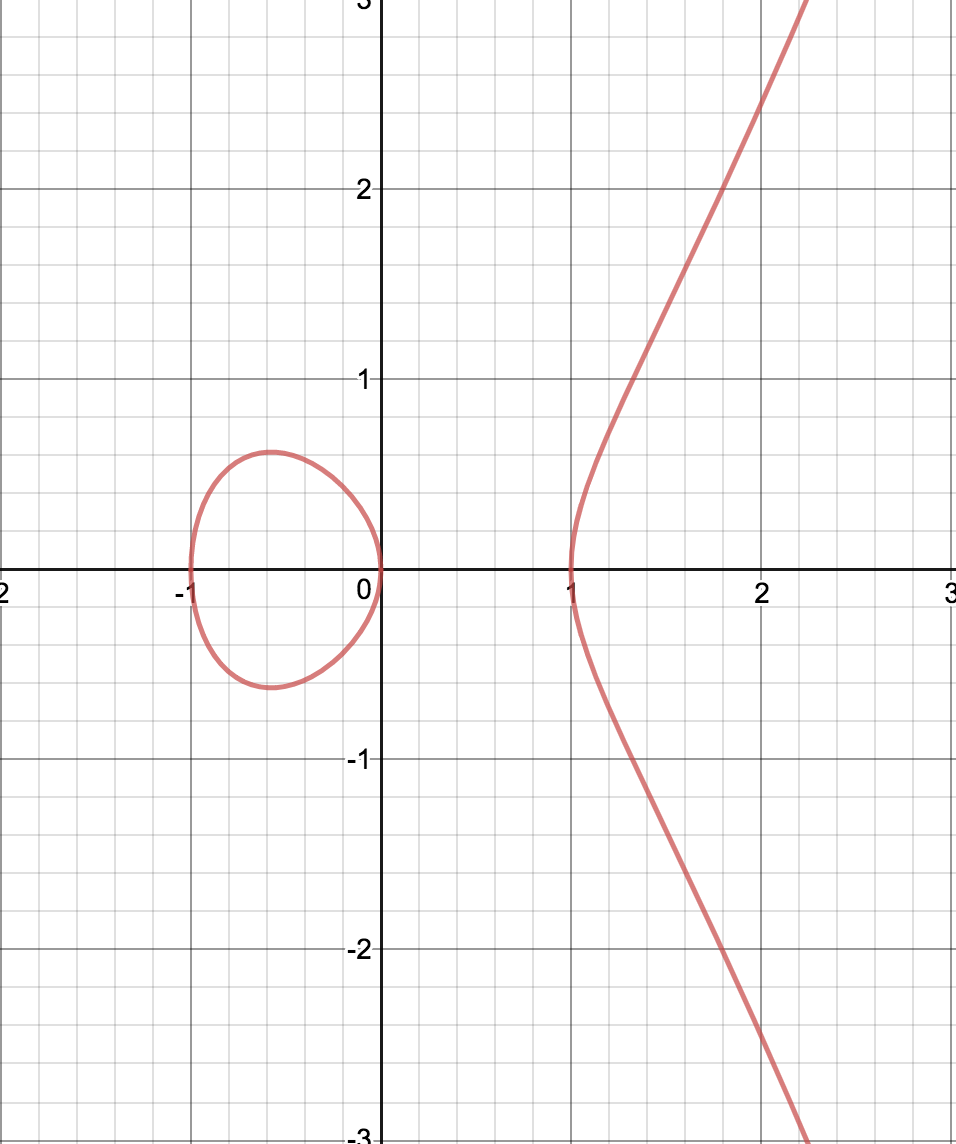
\includegraphics[width=0.3\textwidth]{1.png}
        \caption{The elliptic curve $Y^2=X^3-X$. Plotted in Desmos.}
    \end{figure}
    \item $V(1)$ is just the empty set.
    \item $V(0)=\mathbb{A}^2$.
    \item $V(Y^2-X^2)$ is the union of $Y=X$ and $Y=-X$. 
    \item $V(X^2+Y^2+Z^2-4)$ is just the sphere $S^2\subset\real^3$ of radius 2 centered around the origin.
\end{enumerate}
We can also look at the \ita{common zero-set} of a collection of polynomials. For $S\subseteq K[X_1,\dotsc,X_n]$, we define $V(S):=\{P\in\mathbb{A}\mid F(P)=0\text{ for all }F\in S\}$.\\\\
\underline{Examples}:
\begin{enumerate}
    \item $V(Y^2-X^2,(Y-X)(X+1))=\{(-1,1)\}\cup\{\text{line }Y=X\}$
    \begin{figure}[H]
        \centering
        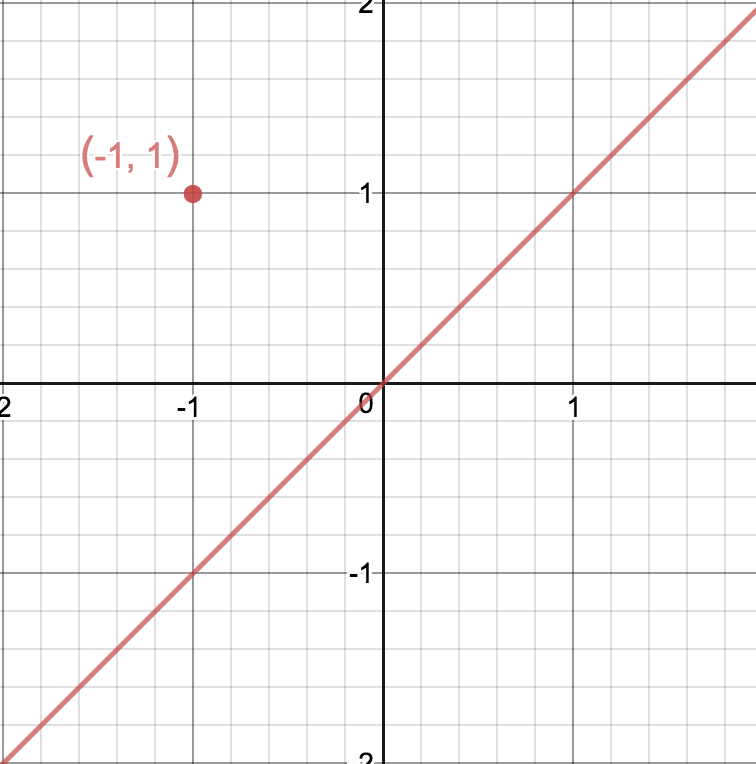
\includegraphics[width=0.3\textwidth]{2.png}
        \caption{$V(Y^2-X^2,(Y-X)(X+1))$. Plotted in Desmos.}
    \end{figure}
    \item $V(X^2+Y^2+Z^2-4,Z-1)$ is the circle $X^2+Y^2+(Z-1)^2=1$.
\end{enumerate}
Note that $V(S)=V(J:=\vbrack{S})$, so we might as well only look at the zero-sets of ideals.
\begin{definition}
    A set $V\subseteq\mathbb{A}^n$ is an \ita{affine algebraic set} over $k$ if $V=V(J)$ for some ideal $J\subseteq k[X_1,\dotsc,X_n]$.
\end{definition}
\begin{remark}
    Some authors use the word \ita{variety} for what we are calling algebraic set. But for us (and Fulton), variety means irreducible algebraic set (to be defined shortly). Make sure to always check which conventions your source follows!
\end{remark}
\underline{Examples}: 
\begin{enumerate}
    \item All of our $V's$ so far in the previous examples are (affine) algebraic sets.
    \item How about the 4 corners of the square centered at the origin: $\{(\pm1,\pm1)\}$?
    \begin{figure}[H]
        \centering
        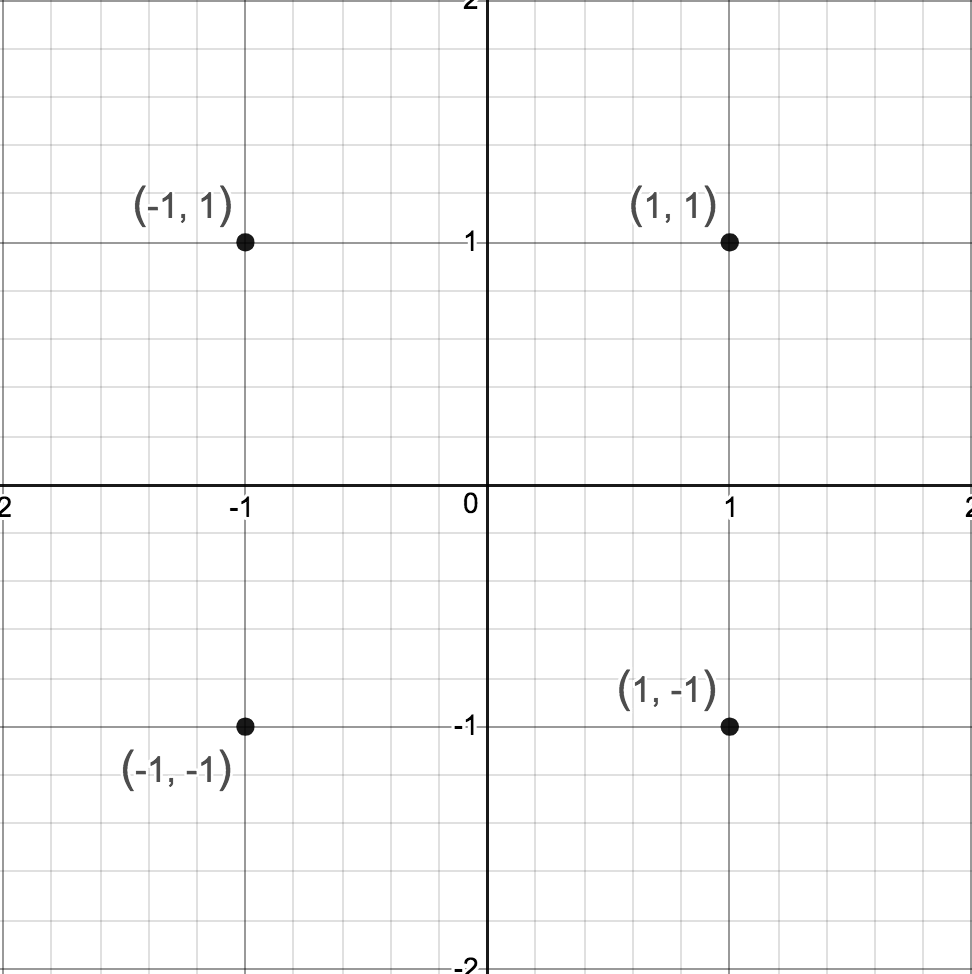
\includegraphics[width=0.2\textwidth]{3.png}
        \caption{The points $\{(\pm1,\pm1)\}$ in the plane. Plotted in Desmos.}
    \end{figure}
    It's $V(Y^2-X^2,X^2+Y^2-2)$.
    \begin{figure}[H]
        \centering
        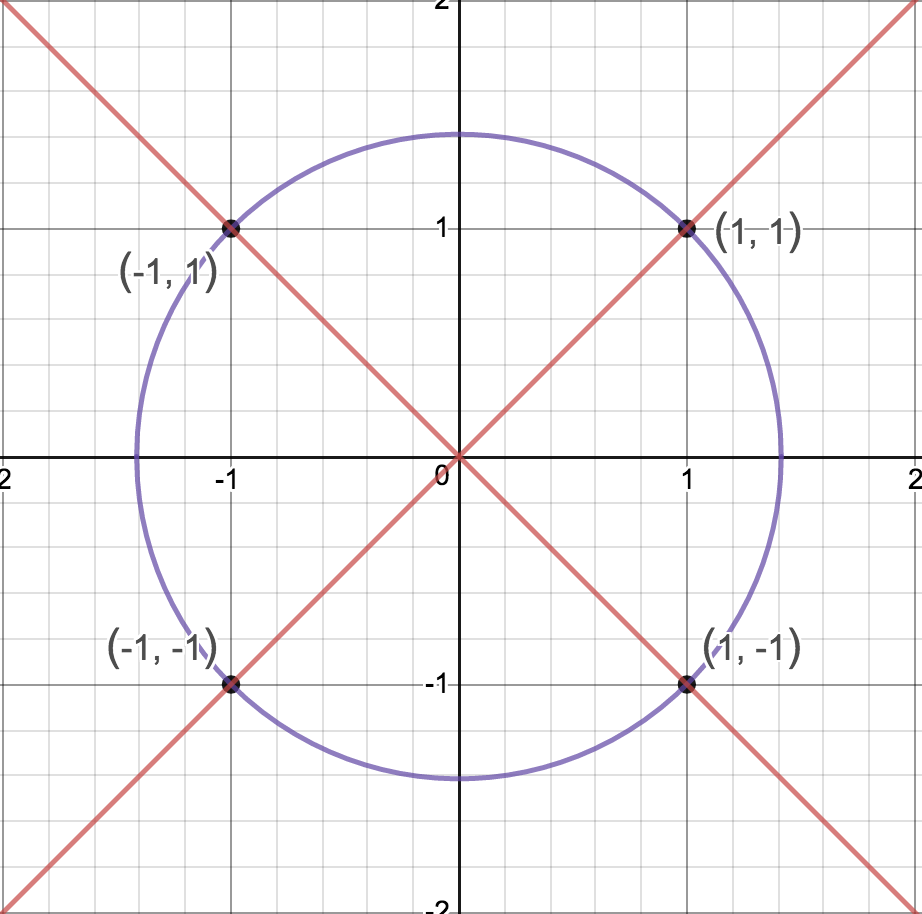
\includegraphics[width=0.3\textwidth]{4.png}
        \caption{$V(Y^2-X^2,X^2+Y^2-2)$. Plotted in Desmos.}
    \end{figure}
    Are there others? $V((X-1)(X+1),(Y-1)(Y+2))$ also works, by Brian's suggestion.
    \begin{figure}[H]
        \centering
        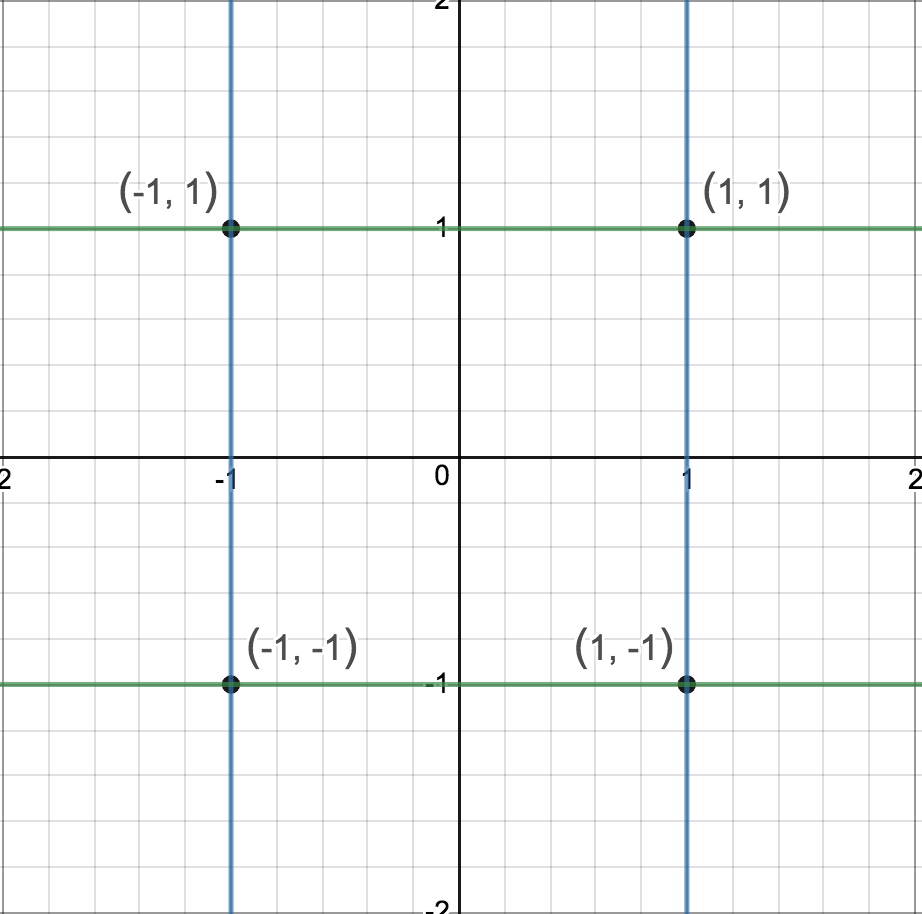
\includegraphics[width=0.3\textwidth]{5.png}
        \caption{Brian's suggestion. Plotted in Desmos.}
    \end{figure}
    \item What are the algebraic sets in $\mathbb{A}^1$? Precisely the finite sets and $\mathbb{A}$ itself.
    \item In $\mathbb{A}^n$, for $k$ algebraically closed (to be defined later), we'll see that $V$ of any non-constant polynomial is infinite.
\end{enumerate}
\begin{theorem}[Theorem for Topologiraffes]
    Topologiraffes is our term for topology.
    \begin{enumerate}
        \item $\emptyset$ and $\mathbb{A}^n$ are algebraic sets.
        \item The union of two algebraic sets is an algebraic set. (So by induction, the union of finitely many is algebraic.)
        \item The intersection of an arbitrary collection is an algebraic set.
    \end{enumerate}
\end{theorem}
\begin{proof}
    $ $ \\
    \begin{enumerate}
        \item $\emptyset=V(1)$, and $\mathbb{A}^n=V(0)$. \checkmark
        \item We claim that $V(I)\cup V( J)=V(IJ)$.
        \item We claim that $\bigcap\limits_{\alpha\in A}V(I_{\alpha})=V\left(\sum\limits_{\alpha\in A}I_{\alpha}\right)$
    \end{enumerate}
    This will be on Homework 03. :)
\end{proof}
\begin{corollary}
    Defining the algebraic sets in $\mathbb{A}^n$ to be closed (and hence their complements to be open) gives us a topology on $\mathbb{A}^n$, called the \ita{Zariski topology}.
\end{corollary}
\begin{remark}
    This is quite different from the usual topology on $\real^n$ or $\cx^n$ derived from the Euclidean metric.
\end{remark}
\subsection{The Ideal Corresponding to an Algebraic Set}
Start with an algebraic set $W\subseteq\mathbb{A}^n$. The set 
\begin{equation}
    I(W):=\{F\in k[X_1,\dotsc,X_n]\mid F(P)=0\text{ for all }P\in W\}
\end{equation}
is an ideal, because it is closed under addition and external multiplication.

Now we have a correspondence from ideals to algebraic sets:
\begin{equation}
    \{\text{ideals }J\subseteq k[X_1,\dotsc,X_n]\}\stackrel{?}{\longleftrightarrow}\{\text{affine algebraic sets }W\subseteq\mathbb{A}^n\}
\end{equation}
By the rules of annihilation on your homework, this correspondence is inclusion-reversing:
\begin{equation*}
    \begin{split}
        J\subseteq K&\implies V(K)\subseteq V(J)\\
        W_1\subseteq W_2&\implies I(W_2)\subseteq I(W_1)
    \end{split}
\end{equation*}
\begin{theorem}
   \begin{enumerate}
        \item $J\subseteq I(V(J))$.
        \item $W\subseteq V(I(W))$.
    \end{enumerate} 
\end{theorem}
\begin{proof}
    The style of proof is the same from the annihilator problems from Homework 01.
\end{proof}
\begin{corollary}{$\varepsilon$}
    \begin{enumerate}
        \item For an $\mathrm{algebraic}$ $\mathrm{set}$ $W$ we have $V(I(W))=W$.
        \item For algebraic sets $W_1\subset W_2$, we have $I(W_2)\subset I(W_1)$.
    \end{enumerate}
\end{corollary}
\begin{proof}
    1 and 2 are from Homework 01, Problems 6c and 6d, respectively.
\end{proof}
For the ideal $J\subseteq k[X_1,\dotsc,X_n]$, is $J=I(V(J))$? Not in general, we can have $J\subset I(V(J))$!

\underline{Example}: Consider $J:=\vbrack{X^2}\subset k[X]$. Then $V(J)=\{0\}\subset\mathbb{A}^1$. Then $I(V(J))=\{\text{all polynomials that vanish at 0}\}=\vbrack{X}$. So $J=\vbrack{X^2}\subset\vbrack{X}=I(V(J))$.

So our correspondence fails to be a bijection, yet...
\section{06 February}
\subsection{Miniquiz}
\subsection{Review of Last Time}
\begin{itemize}
    \item For a set $S\subseteq k[X_1,\dotsc,X_n]$ (we might as well choose $S$ to be an ideal), we set $V(S):=\{P\in\mathbb{A}^n\mid F(P)=0\text{ for all }F\in S\}$.
    \item $V\subset\mathbb{A}^n$ is an (affine) algebraic set if $V=V(J)$ for some ideal $J\subset k[X_1,\dotsc,X_n]$.
    \item For an algebraic set $W\subseteq\mathbb{A}^n$, we set $I(W):=\{F\in K[X_1,\dotsc,X_n]\mid F(P)=0\text{ for all }P\in W\}$.
\end{itemize}
We built a correspondence:
\begin{equation*}
    \{\text{ideals }J\subseteq k[X_1,\dotsc,X_n]\}\stackrel{?}{\longleftrightarrow}\{\text{affine algebraic sets }W\subseteq\mathbb{A}^n\}
\end{equation*}
where $J\mapsto V(J)$ and $W\mapsto I(W)$. Unfortunately, this correspondence is not bijective.
\subsection{Decomposition of Algebraic Sets}
\subsubsection{As intersections of hypersurfaces}
This is fun at first, but ultimately unsatisfying.
\begin{definition}
    A \ita{hypersurface} is an algebraic set that is the zero-set of a single polynomial. Intuitively, a hypersurface has one less dimension than the ambient space.
\end{definition}
\begin{remark}
    We really want to talk about \ita{manifolds}, but unfortunately, this class needs to be self-contained.
\end{remark}
\underline{Examples}:
\begin{enumerate}
    \item For $n=2$, $V(Y-X^2)$ is a parabola.
    \begin{figure}[H]
        \centering
        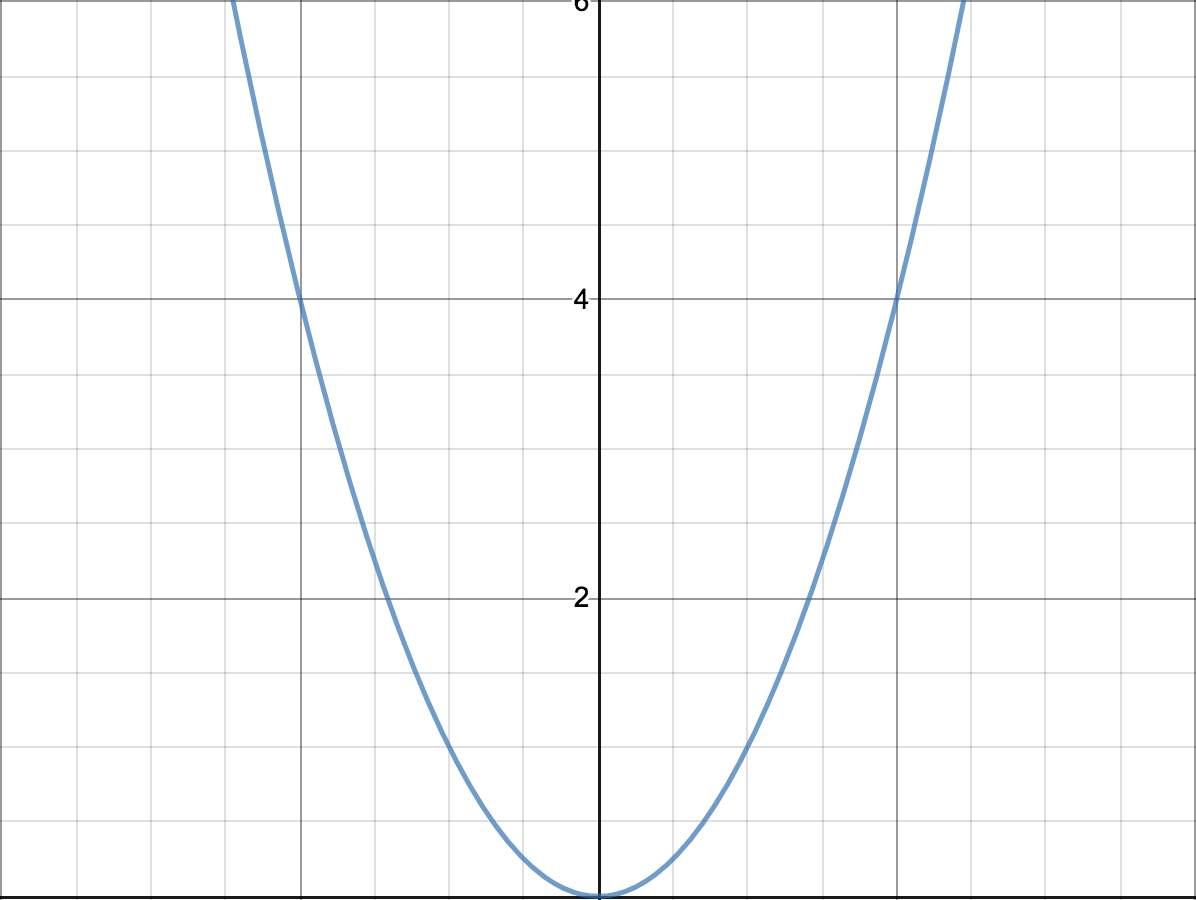
\includegraphics[width=0.3\textwidth]{6.png}
        \caption{$V(Y-X^2)$. Plotted in Desmos.}
    \end{figure}
    \item For $n=3$, $V(X^2+Y^2-Z^2-1)$ is a hyperboloid of one sheet. 
    \begin{figure}[H]
        \centering
        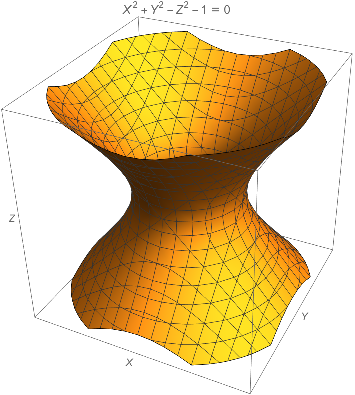
\includegraphics[width=0.3\textwidth]{7.png}
        \caption{$V(X^2+Y^2-Z^2-1)$. Plotted in \ita{Mathematica}.}
    \end{figure}
    \item In $n=3$ again, what is $V(X^2+Y^2-Z^2-1,Z)$? It is the unit circle in the $XY$-plane. 
    \begin{figure}[H]
        \centering
        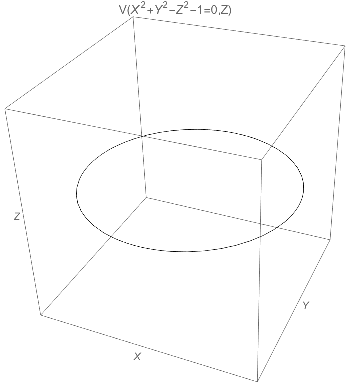
\includegraphics[width=0.3\textwidth]{8.png}
        \caption{$V(X^2+Y^2-Z^2-1,Z)$. Plotted in \ita{Mathematica}.}
    \end{figure}
\end{enumerate}
Intuitively, each polynomial restriction that you impose cuts the dimension down by one. However, this is not always true.
\begin{theorem}
    Every algebraic set can be obtained as a finite intersection of hypersurfaces.
\end{theorem}
\begin{proof}
    Start with an algebraic  $V(J)$ where $J\subseteq k[X_1,\dotsc,X_n]$ is an ideal. By HBT, $J$ is finitely generated by $F_1,\dotsc,F_r\in k[X_1,\dotsc,X_n]$. Thus $V(J)=\bigcap\limits_{i=1}^rV(F_i)$.
\end{proof}
This theorem is not as impressive as it sounds, because the decomposition is not unique. For example, $V(X^2+Y^2-Z^2-1,Z)$ can be written as $V(Z)\cap V(X^2+Y^2-1)$ or as $V(Z)\cap V(X^2+Y^2+Z^2-1)$. For an easier example, $V(X+Y,X-Y)=V(X+Y)\cap V(X-Y)=V(X)\cap V(Y)$.
\subsubsection{As the union of varieties}
\begin{definition}
    A non-empty algebraic set $W$ is \ita{irreducible} if it is not possible to write $W=W_1\cup W_2$, where $W_1,W_2\subsetneq W$ are algebraic sets. An (affine) irreducible algebraic set is called an \ita{(affine) variety}.
\end{definition}
\underline{Examples}: 
\begin{enumerate}
    \item $V(Y^2-X^2)=V(Y+X)\cup V(Y-X)$
    \begin{figure}[H]
        \centering
        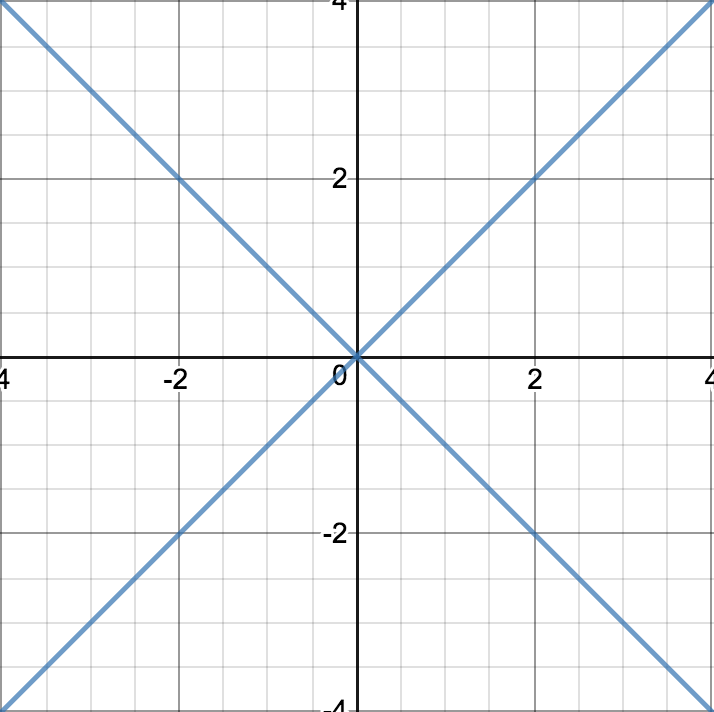
\includegraphics[width=0.3\textwidth]{9.png}
        \caption{$V(Y+X)\cup V(Y-X)$. Plotted in Desmos.}
    \end{figure}
    \item $V(Y-X^2)$ seems like it is irreducible. In fact, it is, but not obviously so.
\end{enumerate}
Proving that an algebraic set is irreducible is often not a trivial task!\\\\
\underline{Algebraic hint}: $Y^2-X^2$ factors into $(Y-X)(Y+X)$. This means that $\vbrack{Y^2-X^2}$ is not a prime ideal in $\real[X,Y]$.
\begin{theorem}
    An algebraic set W is irreducible if and only if I(W) is a prime ideal.
\end{theorem}
\begin{proof}
    Homework 03, Problem 6 :)
\end{proof}
\underline{Example}: Let $F(X,Y):=Y-X^2$, $W:=V(F)\subset\mathbb{A}^2(\real)$. We will show that $W$ is irreducible.\\\\
\textbf{Claim.} $I(W)=\vbrack{F}$.\\\\
To prove this, we will need a helpful lemma.
\begin{lemma}
    Let R be a (unital commutative) ring, and let $b\in R$, $G(Y)\in R[Y]$ such that $G(b)=0$. Then $G(X)=H(Y)(Y-b)$ for some $H(Y)\in R[Y]$.
\end{lemma}
\begin{proof}
    To be proved in a future Homework set :)
\end{proof}
Now let's prove our claim:
\begin{proof}
    Suppose $G(X,Y)\in I(V(F))$. We want to show that $G\in\vbrack{F}$. Define $\overline{G}(X):=G(X,X^2)\in\real[X]$. Then for all $b\in\real$, we have $\overline{G}(b)=G(b,b^2)=0$. So $\overline{G}(X)$ has infinitely many roots, and must be the zero polynomial. Consider $G\in\real[X][Y]$, that is, $G$ as a polynomial in $Y$ with coefficients from $\real[X]$. We have $G(X^2)=\overline{G}(X)=0$, so by the above Lemma (with $R:=\real[X]$), $G$ factors into $G(Y)=H(Y)(Y-X^2)$ for some $H\in\real[X,Y]$ (up to isomorphism). Thus $G\in\vbrack{F}$, so $I(F(V))=\vbrack{F}$, as was claimed.
\end{proof}
Using FIT,
\begin{equation*}
    \begin{split}
        \real[X,Y]/I(W)&=\real[X,Y]/\vbrack{Y-X^2}\\
        &\cong\real[X][Y]/\vbrack{Y-X^2}\\
        &\cong\real[X]
    \end{split}
\end{equation*}
But $\real[X]$ is a domain, so $\vbrack{Y-X^2}$ is a prime ideal, so by Homework 03, $V(Y-X^2)$ is irreducible.
\begin{theorem}
    Every non-empty algebraic set W has a decomposition as a finite union of varieties: $W=\bigcup\limits_{i=1}^nW_i$, where $W_i\not\subseteq W_j$ for any $i\neq j$. Furthermore, this decomposition is unique, in the sense that if $W=\bigcup\limits_{i=1}^nW_i=\bigcup\limits_{j=1}^mZ_j$ with all $W_i$ and $Z_j$ irreducible, then $n=m$ and $W_i=Z_i$ after a suitable permutation.
\end{theorem}
\begin{proof}
    (Uniqueness) Suppose $W=\bigcup\limits_{i=1}^nW_i=\bigcup\limits_{j=1}^mZ_j$. Look at $W_1$ and decompose it over the $Z_j$'s: $W_1=\bigcup\limits_{j=1}^m(W_1\cap Z_j)$. Since $W_1$ is irreducible, it must be that $W_1\cap Z_j=W_1$ for some $j$. After re-indexing, we may assume that $j=1$. So $W_z\cap Z_1=Z_1\iff W_z\subseteq Z_1$. By the same argument, decomposing $Z_1=\bigcup\limits_{i=1}^n(W_i\cap Z_1)$, we get $Z_1\subseteq W_i$ for some $i$. But then $W_1\subseteq Z_2\subseteq W_i$, so $i=1$. Hence $W_1=Z_1$. Similarly, $W_2=Z_2$ after permuting. Continuing in this fashion, we match each $W_i$ with a unique $Z_j$, so $m=n$ and $W_i=Z_i$ for all $i$.
\end{proof}
\section{11 February}
\subsection{Miniquiz}
Is it better to view affine algebraic sets as an intersections of hypersurfaces or as a union of varieties. Why?
\subsection{Last Time}
Some definitions:
\begin{enumerate}
    \item Algebraic set: $W=V(J)$ for some $J\subseteq k[X_1,\dotsc,X_n]$
    \item Variety: irreducible algebraic set, $W\neq W_1\cup W_2$ for $W_i\subsetneq W$
\end{enumerate}
\begin{align*}
    \{\text{ideals }J\subseteq k[X_1,\dotsc,X_n]\}&\stackrel{}{\longleftrightarrow}\{\text{affine algebraic sets }W\subseteq\mathbb{A}^n\}\\
    J&\mapsto V(J):=\{P\in\mathbb{A}^n\mid F(P)=0\text{ for all }F\in J\}\\
    W&\mapsto I(W):=\{F\in k[X_1,\dotsc,X_n]\mid F(P)=0\text{ for all }P\in W\} 
\end{align*}
\begin{theorem}[5.4 from Last Time]
    Every non-empty $W$ decomposes into varieties: $W=\bigcup\limits_{i=1}^nW_i$ for $W_i\not\subset W_j$. Furthermore, this decomposition is unique.
\end{theorem}
\begin{proof}
    (Existence) Start by defining $W_0:=W$. If $W_0$ is irreducible, then we are done. If not, then $W_0=W_1\cup W_2$ for proper algebraic subsets $W_1$ and $W_2$. If both $W_1$ and $W_2$ are irreducible, then done. Otherwise, at least one of them decomposes, say $W_1=W_{1,1}\cup W_{1,2}$, for proper algebraic subsets $W_{1,j}\subsetneq W_1$. If all of the decompositions eventually get to irreducibles in a finite number of steps, then we are done. Otherwise, this will produce an infinite properly descending chain of algebraic sets
    \[W_0\supsetneq W_1\supsetneq W_{1,1}\supsetneq W_{1,1,1}\supsetneq\dotsb.\]
    Take $I$ of everything in the chain. This reverses the inclusions and preserves proper containment:
    \[I(W_0)\subsetneq I(W_1)\subsetneq I(W_{1,1})\subsetneq I(W_{1,1,1})\subsetneq\dotsb\]
    This contradicts the noetherianity of $k[X_1,\dotsc,X_n]$ (by HBT). So we must have a finite decomposition into irreducibles.
\end{proof}
\underline{Example}: In $\real$, try decomposing $V(Y-X^2,X^2+Y^2-2)$.
\begin{figure}[H]
    \centering
    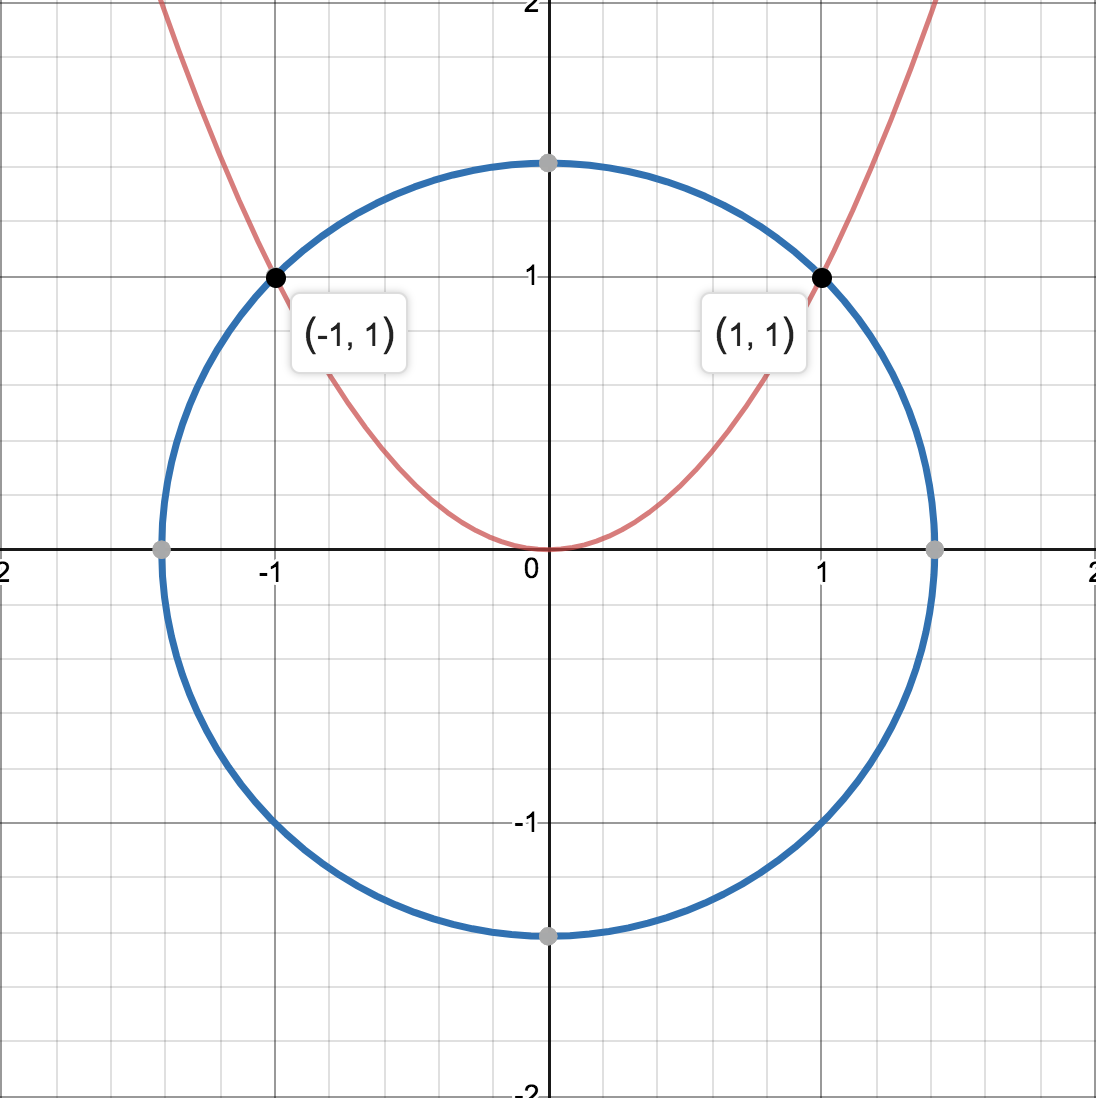
\includegraphics[width=0.3\textwidth]{10.png}
    \caption{$V(Y-X^2,X^2+Y^2-2)$. Plotted in Desmos.}
\end{figure}
We can write $V(X-1,Y-1)\cup V(X+1,Y-1)$.
\begin{figure}[H]
    \centering
    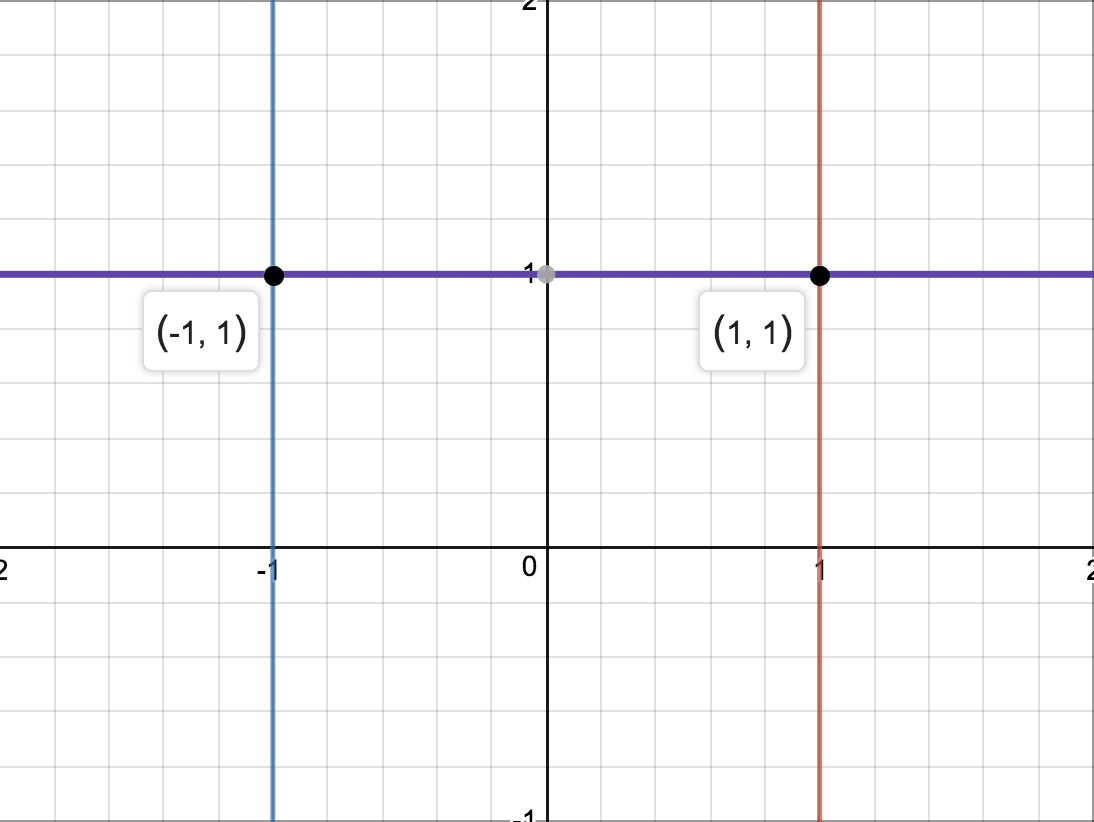
\includegraphics[width=0.3\textwidth]{11.png}
    \caption{$V(X-1,Y-1)\cup V(X+1,Y-1)$. Plotted in Desmos.}
\end{figure}
Note that the polynomials used to define the varieties may not be unique, but the actual sets $\{(1,1)\}$ and $\{(1,-1\}$ \ita{are} unique.

Also note the difference between $V(X-1,Y-1)$ and $V((X-1)(Y-1))$!
\begin{figure}[H]
    \centering
    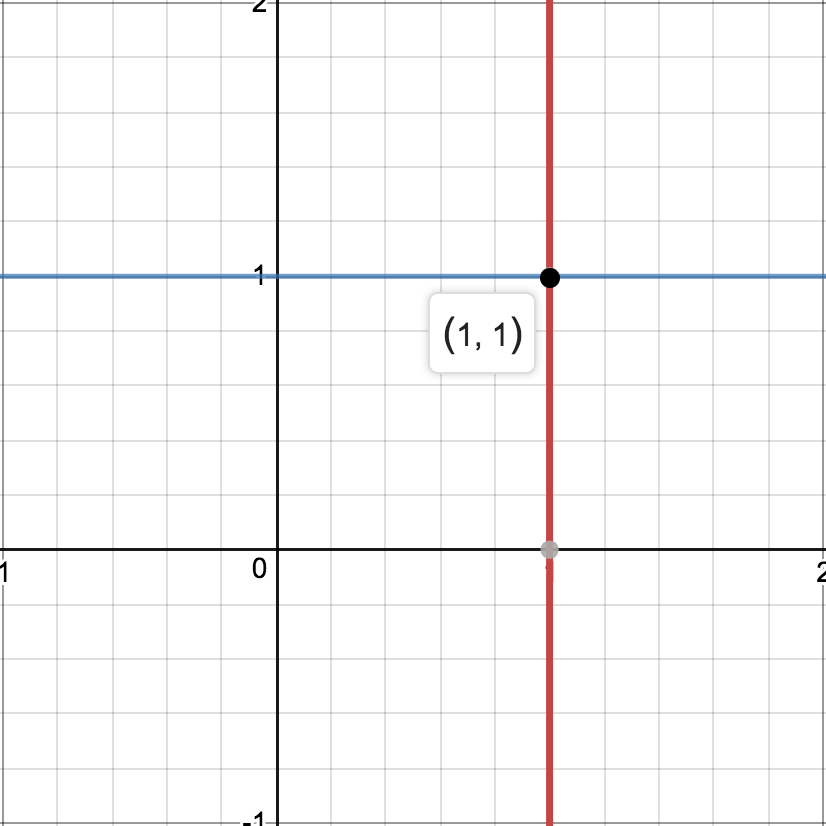
\includegraphics[width=0.3\textwidth]{12.png}
    \caption{The point $V(X-1,Y-1)=(1,1)$, while $V((X-1)(Y-1))$ corresponds to the lines $X=1$ and $Y=1$ . Plotted in Desmos.}
\end{figure}
\subsection{Algebraicity}
\begin{definition}
    Let $k\subseteq K$ be fields. $\alpha\in K$ is said to be \ita{algebraic over k} if $\alpha$ is a root of a polynomial in $k[X]$ (which we can take to be \ita{monic}, \ita{i.e.}, leading coefficient equal to 1). $\alpha$ is said to be \ita{transcendental over k} if it is not algebraic over $k$. $K$ is said to be \ita{algebraic over k} if every $\alpha\in K$ is algebraic over $k$.
\end{definition}
\underline{Examples}: For these, let $k:=\q$.
\begin{enumerate}
    \item For $K:=\real$, $\sqrt{2}$ is algebraic over $\q$, since it is a root of the polynomial $X^2-2$. $\phi:=\frac{1+\sqrt{5}}{2}$, the golden ratio, is algebraic over $\q$, since it is the root of the polynomial $X^2-X-1$. 
    \item For $K:=\cx$, $i$ is a classic example.
    \item $\pi$ and $e$ are transcendental, but this is quite difficult to prove.
    \item Try $K:=\q[\sqrt{2}]=\{a+b\sqrt{2}\mid a,b\in\q\}$. This is algebraic over $\q$.
    \item Note that $\real$ and $\cx$ are not algebraic over $\q$. However, $\cx$ \ita{is} algebraic over $\real$.
\end{enumerate}
These examples show that the choice of the field $k$ is very important, much more so than the choice of the field $K$.
\begin{theorem}
    Let $k$ be a field. The following are equivalent and define being $\mathrm{algebraically}$ $\mathrm{closed}$.
    \begin{enumerate}
        \item k has no proper algebraic extension, i.e., there does not exist a field $K\supset k$ algebraic.
        \item Every nonconstant polynomial over k factors into linear factors.
    \end{enumerate}
\end{theorem}
\underline{Examples}:
\begin{enumerate}
    \item $\q$ is not algebraically closed, since $X^2-2$ has no root in $\q$.
    \item $\real$ is also not algebraically closed, since $X^2+1$ has no root in $\real$.
    \item $\cx$ is algebraically closed. This is the Fundamental Theorem of Algebra!
    \item $\z_5$ is not algebraically closed, since $X^2-2$ has no root. In fact, no \ita{finite} field is algebraically closed.
\end{enumerate}
\begin{theorem}
    Every algebraically closed field is infinite.
\end{theorem}
\begin{proof}
    Homework :)
\end{proof}
You would like to start with a field and close it by throwing in roots of all polynomials. But then you can make more polynomials, so you need more roots.
\begin{figure}[H]
    \centering
    
\includegraphics[width=0.3\textwidth]{13.png}
    \caption{This is what happens when you try to make a finite field algebraically complete.}
\end{figure}
\begin{theorem}
    Every field has an $\mathrm{algebraic}$ $\mathrm{closure}$, that is, a field with the properties:
    \begin{enumerate}
        \item $\overline{k}$ is algebraic over $k$.
        \item $\overline{k}$ is algebraically closed.
    \end{enumerate}
\end{theorem}
Rejoice that $\overline{k}$ even exists. $\overline{k}$ is small enough to be algebraic over $k$, but big enough to be algebraically closed. The proof of this theorem uses Zorn's Lemma.\\\\
\underline{Examples}:
\begin{enumerate}
    \item $\cx$ is an algebraic closure of $\real$, but it is not a an algebraic closure of $\q$. 
    \item The algebraic closure of $\q$ is a subset of $\cx$, but is its relatively small (only countable) and quite mysterious. It is $\mathbb{A}$, the algebraic numbers.
    \item The algebraic closure of $\z_p$ is the union of all $\field_{p^n}$ (the finite field of order $p^n$). It is infinite.
\end{enumerate}
\begin{remark}
    The overline notation here always means \ita{algebraic} closure, so $\overline{\q}=\mathbb{A}$. This is not to be confused with \ita{topological} closure! ($\overline{\q}=\real$ topologically with respect to the standard topology on $\real$).
\end{remark} 
\section{13 February}
\subsection{Miniquiz}
Use the definition of algebraicity to show that $\omega:=\frac{1+i\sqrt{3}}{2}$ is algebraic over $\q$.
\subsection{Fixing the Imperfect Correspondence}
We've been harping about the correspondence below:
\[\{\text{ideals}\}\stackrel{}{\longleftrightarrow}\{\text{algebraic sets}\}.\]
We know that $W=V(I(W))$. But $J\subseteq I(V(J))$ can be proper, as with $J:=\vbrack{X^2}\subsetneq\vbrack{X}=I(V(J))$. This typifies the general problem: If $J\subseteq k[X_1,\dotsc,X_n]$ and $F^m\in J$ for some $m>1$, then for any $P\in V(J)$, we will have $[F(P)]^m=0$, so $F(P)=0$, and $F\in I(V(J))$ even if $F$ itself is not in $J$.\\\\
\underline{Conclusion}: $J\subseteq\sqrt{J}\subseteq I(V(J))$, so if $J\subsetneq\sqrt{J}$, then the correspondence breaks down.
\begin{definition}
    Let $J\subseteq R$ be an ideal. The \ita{radical of J} is the set
    \begin{equation}
        \sqrt{J}:=\{r\in R\mid r^m\in J\text{ for some }m\geq1\}
    \end{equation}
    We say $J$ is a \ita{radical ideal} if $J=\sqrt{J}$.
\end{definition}
We always have $J\subseteq\sqrt{J}$, but not equality in general. For example, let $J:=\vbrack{60}\subset\z$. Then $J\subsetneq\vbrack{30}=\sqrt{J}$.
\begin{theorem}[Hilbert's Nullstellensatz]
    Let k be algebraically closed, and let $R:=k[X_1,\dotsc,X_n]$. Let $J\subseteq R$ be an ideal.
    \begin{enumerate}
        \item If $J\subsetneq R$, then $V(J)\neq\emptyset$.
        \item Every maximal ideal $\mathfrak{m}\subsetneq R$ has the form $\mathfrak{m}=\vbrack{x_1-a_1,\dotsc,x_n-a_n}$ for some specific point $(a_1,\dotsc,a_n)\in\mathbb{A}^n$.
        \item $I(V(J))=\sqrt{J}$. So if $J$ is itself a radical ideal, then $I(V(J))=J$. 
    \end{enumerate}
\end{theorem}
\begin{remark}
    1 and 2 are equivalent and are collectively called the \ita{Weak Nullstellensatz}. We will prove them first, and then use 2 to prove 3, which is called the \ita{Strong Nullstellensatz}. However, we have to learn some more machinery before starting this proof.
\end{remark}
\underline{Examples}: We will show just why it is important for $k$ to be algebraically closed. For the following examples, take $J:=\vbrack{X^2+1}$.
\begin{enumerate}
    \item Take $k:=\real$. Then $J\subsetneq\real[X]$, but so $V(J)=\emptyset$.
    \item Take $k:=\cx$. Note that $J$ \ita{is} maximal, because $\real[X]/J\cong\cx$ is a field. However, it is not of the form $\vbrack{X-a}$ for any $a\in\real$. If it did, then $a\in V(J)$, and thus $V(J)\neq\emptyset$.
    \item Back in $k:=\real$, $V(J)=\emptyset$, so $I(V(J))=I(\emptyset)=\real[X]$. However, $J$ \ita{is} radical (because maximal $\Rightarrow$ prime $\Rightarrow$ radical), so $\vbrack{J}=J$, but $I(V(J))\neq J$.
\end{enumerate}
Our continuing assumption from here on out is that $k$ is a field that is not necessarily algebraically closed.
\begin{definition}
    A \ita{k-algebra} is a (unital and commutative) ring that contains $k$ as a subring.
\end{definition}
\begin{remark}
    This definition of a $k$-algebra starts from the ring $R$, instead of equipping a vector space with a binary operation $m:V\times V\to V$. For our purposes, we need to cut to the chase and assume associativity, existence of an identity element, and commutativity.
\end{remark}
\underline{Examples}:
\begin{enumerate}
    \item $k[X_1,\dotsc,X_n]$ is a $k$-algebra.
    \item $\cx$ is an $\real$-algebra.
    \item $\mathbb{H}$ is an $\real$-algebra, but since it is not commutative, we sadly have to leave it out of the discussion.
\end{enumerate}
\begin{definition}
    If $R$ and $S$ are $k$-algebras, then a \ita{k-algebra homomorphism} is a ring homomorphism $\phi:R\to S$ that is the identity on $k$, \ita{i.e.}, $\phi(\alpha)=\alpha$ for all $\alpha\in k$.
\end{definition}
\underline{Examples}: 
\begin{enumerate}
    \item To define a $\q$-algebra homomorphism $\phi:\q[x]\to\real$, we only need to specify $\phi(X)$. In essence, $\phi$ is an evaluation of the polynomial as a function of $X$.
    \begin{enumerate}
        \item Let $\phi(X):=\sqrt{2}$. Then $\ker\phi=\vbrack{X^2-2}$.
        \item Let $\phi(X):=\pi$. Then $\ker\phi=\{0\}$ (because $\pi$ is transcendental), so $\phi$ is injective. Then $\q[X]\cong\text{Im}\phi$.
    \end{enumerate}
    \item Try $\phi:\cx\to\cx$, defined by $\phi:i\mapsto-i$. This is an $\real$-algebra homomorphism, and is just complex conjugation. In addition, complex conjugation is an automorphism, and is in fact the only \ita{continuous} automorphism of $\cx$ aside from the identity.
\end{enumerate}
A $k$-algebra is \ita{generated as a k-algebra} by a set $\{a_i\}_{i\in I}$ if every element of $R$ can be written as a sum of products of $k$ and $a_i$'s, \ita{i.e.}, as a polynomial over $k$ in the $a_i$'s. We write $R=k[a_i]_{i\in I}$. This is not the same as the free polynomial algebra $k[X_i]_{i\in I}$, because the $a_i$'s might satisfy some relation, whereas the $X_i$'s do not (``free'' means exactly this). \\\\
\underline{Examples}: 
\begin{enumerate}
    \item $\cx=\real[i]$, but we know that $\cx\not\cong\real[X]$ because $i$ satisfies the relation $i^2+1=0$, while not so for $X^2+1=0$ in $\real[X]$.
    \item For a non-commutative example, the real Clifford algebra $C\ell_{p,q}(\real)=\real[E_1,\dotsc,E_{2^n-1}]$ (here $E_i=e_i$ for $i=1,\dotsc,n$, and for $i>n$, they are the successive exterior products of the $e_i$'s), but $C\ell_{p,q}(\real)\not\cong\real[X_1,\dotsc,X_{2^n-1}]$, since the $e_i$'s satisfy an important anticommutation relation: $\{e_i,e_j\}=2\eta_{ij}$. 
    \item For an even crazier example, the octonions $\mathbb{O}$ can be written as $\real[e_1,\dotsc,e_7]$, but clearly $\mathbb{O}\not\cong\real[X_1,\dotsc,X_7]$ because the octonions aren't even associative!
\end{enumerate}
In a sense, polynomial rings are the mother of all algebras.\\\\
\underline{Examples}: 
\begin{enumerate}
    \item $\cx$ is a quotient of $\real[X]$ under $X\mapsto i$. So $\cx\cong\real[X]/\vbrack{X^2+1}$.
    \item $\q[\sqrt{2}]$ is a quotient of $\q[X]$ under $X\mapsto\sqrt{2}$. So $\q[\sqrt{2}]\cong\q[X]/\vbrack{X^2-2}$.
    \item $\q[\pi]$ is a $\q$-subalgebra of $\real$. So it s a quotient of $\q[X]$ under $X\mapsto\pi$. Since $\ker\phi=\{0\}$, $\q[\pi]\cong\q[X]$ (in a sense, $\q$ doesn't ``see'' $\pi$ since it is transcendental, and so it gets treated just like a free variable).
\end{enumerate}
$R$ is a \ita{finitely generated} $k$-algebra if it can be generated by a finite set $\{a_1,\dotsc,a_n\}$. Equivalently, $R$ is quotient of the polynomial ring $K[X_1,\dotsc,X_n]$.\\\\
\underline{Examples}:
\begin{enumerate}
    \item All of our examples so far have been finitely generated $k$-algebras.
    \item $\cx$ is not a finitely generated $\q$-algebra. This is not easy to prove.
    \item $k[X_1,X_2,\dotsc,]$ is not finitely generated.
\end{enumerate}
\begin{lemma}[Zariski's Lemma]
    Let k be a field and let $K=k[X_1,\dotsc,X_n]$ be a finitely generated $k$-algebra that is itself a field. Then $K$ is algebraic over $k$.
\end{lemma}
\section{18 February}
\subsection{Miniquizzes}
\begin{enumerate}
    \item Let $\wp\subseteq R$ be a prime ideal. Then 
    \item Will get back to this later.
\end{enumerate}
\subsection{Hilbert's Nullstellensatz}
\begin{theorem}[Hilbert's Nullstellensatz]
    Let k be algebraically closed. Let $R:=k[X_1,\dotsc,X_n]$, and let $J\subseteq R$ be an ideal.
    \begin{enumerate}
        \item If $J\subset R$ is proper, then $V(J)\neq\emptyset$.
        \item Every maximal ideal $\mathfrak{m}\subset R$ is of the form $\mathfrak{m}=\vbrack{X_1-a-1,\dotsc,X_n-a_n}$ for some $(a_1,\dotsc,a_n)\in\mathbb{A}^n(K)$.
        \item $I(V(J))=\sqrt{J}$.
    \end{enumerate}
\end{theorem}
Here is the plan to proving this:
\begin{enumerate}[(A)]
    \item Prove that $1\Leftrightarrow2$. (Homework)
    \item Prove 2 independently. This will require Zariski's Lemma: If $K$ is a $k$-algebra that is itself a field, then $\mathbb{K}$ is algebraic over $K$.
    \item Prove that $1\Rightarrow3$. This will use something called Rabinowitsch's trick. Ironically, Rabinowitsch was not even a real person!
\end{enumerate}
\subsection{Part (B)}
First note that an ideal of the form $\vbrack{X_1-a_1,\dotsc,X_n-a_n}$ is indeed maximal, because $k[X_1,\dotsc,X_n]/\vbrack{X_1-a_1,\dotsc,X_n-a_n}\cong K$ is a field.

Let $\mathfrak{m}\subsetneq R$ be a maximal ideal. Then $\mathbb{K}:=R/\mathfrak{m}$ is a field. Let $\pi:R\twoheadrightarrow R/\mathfrak{m}$ be the canonical surjection $\pi(r):=\overline{r}$. $\mathbb{K}$ is a finitely generated $K$-algebra, since it is a quotient of $k[X_1,\dotsc,X_n]$, \ita{i.e.}, $K$ is finitely generated by $\pi(X_1),\dotsc,\pi(X_n)$. By Zariski's Lemma, $K$ is algebraic over $k$. But since $k$ is algebraically closed, $K=k$. This means $\pi(X_1)=a_1$ for some $a_1\in K$. Then $X_1-a_1\in\ker\pi=\mathfrak{m}$. Similarly, $X_i-a_i\in\mathfrak{m}$ for all $i=1,\dotsc,n$. Then $\vbrack{X_1-a_1,\dotsc,X_n-a_n}\subseteq\mathfrak{m}$. Since $\vbrack{X_1-a_1,\dotsc,X_n-a_n}$ is maximal, it is equal to $\mathfrak{m}$. $\qed$
\subsection{Part (C)}
Let $J\subseteq R:=k[X_1,\dotsc,X_n]$ be an ideal. By HBT, $J$ is finitely generated; say $J=\vbrack{F_1,\dotsc,F_m}$. Since $\sqrt{J}\subseteq I(V(J))$, it suffices to show that $I(V(J))\subseteq\sqrt{J}$. 

Let $F\in I(V(J))$. Then $F$ vanishes on every $P\in\mathbb{A}^n(k)$ for which $F_1,\dotsc,F_m$ are zero. We want to show that $F^r\in J$ for some $r\in\z^+$.\\\\
\textbf{Rabinowitsch's Trick.} Introduce an additional variable $X_{n+1}$ and consider the ring $R':=k[X_1,\dotsc,X_n,X_{n+1}]$. In $R'$, consider the ideal $J':=\vbrack{F_1,\dotsc,F_m,1-X_{n+1}F}$. Let $P':=(a_1,\dotsc,a_n,a_{n+1})\in\mathbb{A}^{n+1}(K)$ be any common zero of $J'$. Note that $F_1,\dotsc,F_m$ only contain the variables $X_1,\dotsc,X_n$, so we have $F_i(a_1,\dotsc,a_n)=0$. By assumption, $F(a_1,\dotsc,a_n)=0$. But then 
\begin{align*}
    (1-X_{n+1}F)(P')&=1-a_{n+1}F(a_1,\dotsc,a_n)\\
    &=1-0\\
    &=1\\
    &\neq0.
\end{align*}
So $P'$ is not a zero of $1-X_{n+1}F$, and hence is not a common zero of $J'$. Thus $P'$ does not exist, and so $J'$ has no common zeros. Thus $V(J')=\emptyset\subset\mathbb{A}^{n+1}(k)$. By the Weak Nullstellensatz 1 (contrapositive), $J'=R'$. So $1\in J'$, and we have the following equation:
\[G_1F_1+\dotsb+G_mF_m+G_{m+1}(1-X_{n+1}F)=1,\]
For $G_i\in R'$.

Introduce a temporary substitution: let $\frac{1}{Y}:=X_{n+1}$. Then
\begin{align*}
    G_1\left(X_1,\dotsc,X_n,\frac{1}{Y}\right)F_1&+\dotsb+G_m\left(X_1,\dotsc,X_n,\frac{1}{Y}\right)F_m\\
    &+G_{m+1}\left(X_1,\dotsc,X_n,\frac{1}{Y}\right)\left(1-\frac{1}{Y}F\right)=1.
\end{align*}
To clear the denominators, multiply by $Y$ raised to the highest power of $\frac{1}{Y}$ that appears in the above equation. For example, if $G_1\left(X_1,X_2,\frac{1}{Y}\right)=X_1X_2+\frac{X_1^2}{Y}+\frac{X_1X_2^3}{Y^2}$, multiplying by $Y^2$ converts it to $\Tilde{G}(X_1,X_2,Y)=X_1X_2Y^2+X_1^2Y+X_1X_2^3$.

Then we have
\[\Tilde{G_1}(X_1,\dotsc,X_n,Y)F_1+\dotsb+\Tilde{G}_m(X_1,\dotsc,X_n,Y)F_m+\Tilde{G}_{m+1}(X_1,\dotsc,X_n,Y)(Y-F)=Y^r.\]
Now substitute in $F$ for $Y$:
\[\Tilde{G_1}(X_1,\dotsc,X_n,F)F_1+\dotsb+\Tilde{G}_m(X_1,\dotsc,X_n,F)F_m+0=F^r.\]
Since $F$ is a polynomial in $X_1,\dotsc,X_n$ only, each $\Tilde{G}_i(X_1,\dotsc,X_n,F)$ is also a polynomial in $X_1,\dotsc,X_n$. Thus we are back to $R=K[X_1,\dotsc,X_n]$, and $F^r\in\vbrack{F_1,\dotsc,F_m}=J$. So $F\in\sqrt{J}$, as desired. $\qed$\\\\
For $k$ algebraically closed, the Nullstellensatz hath bestown upon us a perfect one-to-one correspondence:
\begin{equation}
    \begin{split}
        \{\text{radical ideals }J\subseteq K[X_1,\dotsc,X_n]\}&\longleftrightarrow\{\text{algebraic sets }W\subseteq\mathbb{A}^n(K)\}\\
        J&\mapsto V(J)\\
        I(W)&\mapsfrom  W\\
        \{0\}&\longleftrightarrow\mathbb{A}^n(K)\\
        \vbrack{F}&\longleftrightarrow\text{ hypersurfaces }\\
        \text{ prime ideals }&\longleftrightarrow\text{ varieties }\\
        \text{ maximal ideals }&\longleftrightarrow\text{ finite sets }\\
        K[X_1,\dotsc,X_n]&\longleftrightarrow\emptyset
    \end{split}
\end{equation}
\section{20 February}
\subsection{Miniquiz}
For the algebraic set $W:=\{(2,1,7)\}\subset\mathbb{A}^3(\cx)$, find the corresponding ideal $I(W)\subseteq\cx[X,Y,Z]$.
\subsection{Some Algebraic Geometry for Today}
\begin{definition}
    Let $V\subseteq\mathbb{A}^n$ be a variety and let $\lambda:V\to K$ be a function. $\lambda$ is said to be a \ita{polynomial function} if there exists a polynomial $F\in k[X_1,\dotsc,X_n]$ such that $\lambda(P)=F(P)$ for all $P\in V$.
\end{definition}
\underline{Example}: Let $V:=V(Y-X^2)\subset\mathbb{A}^2(\real)$, and define $\lambda:V\to\real$ by $\lambda(X,Y):=5Y^{3/2}$. $\lambda$ doesn't look like a polynomial, but for $P\in V$, we have $\lambda(P)=F(P)$, where $F(X,Y):=5X^3\in\real[X,Y]$. Hence $\lambda$ is a polynomial function. It is also true that $\lambda(P)=G(P)$, where $G(X,Y):=5XY\in\real[X,Y]$. They both work because $F$ and $G$ are equivalent on $V$. In fact,
\begin{align*}
    F(X,Y)-G(X,Y)&=5X^3-5XY\\
    &=-5X(Y-X^2)\\
    &\in I(V). \checkmark
\end{align*}
In general, to create a polynomial function, start with a polynomial $F\in k[X_1,\dotsc,X_n]$, but acknowledge that $F$ and $G$ will give the same function if and only if $F-G\in I(V)$.
\begin{definition}
    The \ita{coordinate ring} of a variety $V\subseteq\mathbb{A}^n$ is 
    \begin{equation}
        \Gamma(V):=k[X_1,\dotsc,X_n]/I(V).
    \end{equation}
\end{definition}
\begin{theorem}
    $\Gamma(V)$ is a domain.
\end{theorem}
\begin{proof}
    $V$ is irreducible, so $I(V)$ is prime. Done!
\end{proof}
\underline{Example}: $V(Y-X^2)$ is irreducible, and $\Gamma(V)=k[X,Y]/\vbrack{Y-X^2}\cong k[X]$ is a domain.
\subsection{Quotient Fields}
Starting with an integral domain $R$, we can form its \ita{quotient field}, also known as its \ita{field of fractions}:
\begin{equation}
    Q:=\{(r,s)\mid r\in R,s\in R\backslash\{0\}\}/\sim,
\end{equation}
where $(r_1,s_1)\sim(r_2,s_2)$ if and only if $r_1s_2=r_2s_1$. Define addition and multiplication in a familiar way:
\begin{equation}
    \begin{split}
        (r_1,s_1)+(r_2,s_2)&:=(r_1s_2+s_2r_1,s_1s_2)\\
        (r_1,s_1)(r_2,s_2)&:=(r_1r_2,s_1s_2).
    \end{split}
\end{equation}
(18) should look familiar: this is how we add and multiply fractions!

It is straightforward but tedious to check that $Q$ is indeed a field containing $R$ as a subring by identifying $r\mapsto(r,1)$.
\begin{remark}
    Quotient fields should not be confused with quotient rings. Beware the confusing terminology!
\end{remark}
\underline{Examples}:
\begin{enumerate}
    \item Let $R:=\z$. Then $Q=\q$.
    \item Let $R:=k[X]$. Then $Q=k(X)$ is the field of \ita{rational functions} over $k$, where elements have the form $\frac{F(X)}{G(X)}$ for $F,G\in k[X]$.
    \item If $R$ is a field, then $Q=R$, because $(r,s)=(rs^{-1},1)$.
    \item Sometimes you don't go all the way to the field of fractions: you stop early at a \ita{local ring}.
\end{enumerate}
Recall that every ring contains maximal ideals. Even fields have one: $\{0\}$.
\begin{definition}
    R is a \ita{local ring} if it has exactly one maximal ideal.
\end{definition}
\underline{Examples}:
\begin{enumerate}
    \item $\z$ is not local, because any $\vbrack{p}$ is maximal.
    \item Any field is local, because the only proper ideal is $\{0\}$!
    \item $R:=\z_{27}$ is local, in fact its only ideals are listed below!
    \[\vbrack{0}\subsetneq\vbrack{9}\subsetneq\vbrack{3}\subsetneq R.\]
    Note that having only finitely many ideals makes $R$ both noetherian and artinian. In general, $\z_{p^n}$ is local for $p$ prime, $\n\in\z^+$.
    \item Let $R:=\{a/b\in\q\mid\gcd(a,b)=1\text{ and }b\text{ is odd }\}$. For homework, you will show that $R$ is a local ring and find its maximal ideal.
    
    This example is quite intriguing. It works essentially because the product of two odd integers is odd. How do we generalize this example?
\end{enumerate}
\subsection{How to Make a Local Ring}
Start with any ring, and localize it. This instruction is as helpful as it is accurate.

For a more helpful set of directions, start with a ring $R$ (preferably a domain, but not necessarily so). Decide on a subset $S$ that you would like to use as denominators, so they will be invertible in a new ring $Q$. (For example, in $R:=\{a/b\in\q\mid\gcd(a,b)=1\text{ and }b\text{ is odd }\}$, $S=1+2\z$.) Then define
\begin{equation}
    Q:=\{(r,s)\mid r\in R,s\in S\}/\sim,
\end{equation}
We need to choose $S$ carefully. We want the following to be true:
\begin{enumerate}
    \item $1\in S$, so we get $R\subseteq Q$ under $r\mapsto(r,1)$.
    \item For the arithmetic to work in $Q$, $S$ must be closed under multiplication.
\end{enumerate}
\begin{definition}
    $S$ is said to be a \ita{multiplicative subset} if
    \begin{enumerate}
        \item $1\in S$, and
        \item $S$ is closed under (internal) multiplication: $s,t\in S\implies st\in S$.
    \end{enumerate}
\end{definition}
\begin{remark}
   This definition makes ideals a poor choice for $S$, since any ideal that contains $1$ is necessarily the whole ring.
   
   $S$ is essentially a multiplicative submonoid of $R$. In fact, we would like to keep $S$ only a monoid, since choosing $S$ to be the multiplicative group of units $R^{\times}$ does nothing!
\end{remark}
We have two ways to generate multiplicative subsets:
\begin{enumerate}
    \item Choose any $s\in R$, and let $S:=\{1,s,s^2,\dotsc\}$.
    \item Choose a prime ideal $\wp\subset R$ and take $S$ to be its complement: $S:=R\setminus\wp$. This works perfectly!
    \begin{enumerate}
        \item $1\in S$, since $\wp\subsetneq R$.
        \item If $a,b\in S$, $ab\in S$.
    \end{enumerate}
\end{enumerate}
Once you have a multiplicative subset $S\subseteq R$, you can \ita{localize}.
\begin{definition}
    We define the \ita{ring of quotients} (not quotient ring!) or \ita{ring of fractions} as follows:
    \begin{equation}
        RS^{-1}:=\{(r,s)\mid r\in R,s\in S\}/\sim,
    \end{equation}
    where $(r_1,s_1)\sim(r_2,s_2)$ if and only if there exists $s\in S$ with $s(r_1s_2-r_2s_1)=0$. Define addition and multiplication just as before with quotient fields. $RS^{-1}$ is still a ring.
\end{definition}
\begin{remark}
   There is an important difference from the case where $R$ is a domain. We're making elements of $S$ invertible. So if $s\in S$ kills something, \ita{i.e.}, $sa=0$, then $a=0$. We establish the modification to $\sim$ to make this true. Also, we don't necessarily have $R\subseteq RS^{-1}$ anymore, because $r\mapsto(r,1)$ might end up being 0.
\end{remark}
Does localization produce a local ring? Sadly, not necessarily. For a counterexample, consider $R:=\z$ and $S:=\{1,2,4,8,\dotsc\}$.
\section{25 February}
\subsection{Miniquiz}
Is the ring $\z_{12}$ local? Justify your answer.
\subsection{Finishing Up the Algebraic Timeout}
Recall the following definitions from last time:
\begin{itemize}
    \item A domain $R$ has a \ita{field of fractions} $Q:=\{(r,s)\mid r\in R,s\in R\setminus\{0\}\}/\sim$. But we don't have to go all the way to $Q$.
    \item A \ita{local} ring has a unique maximal ideal.
    \item Given a \ita{multiplicative subset} $S\subseteq R$, we can form the ring of fractions $RS^{-1}:=\{(r,s)\mid r\in R,s\in S\}/\sim$. But it is not always local. However, localizing a \ita{prime} ideal does produce a local ring.
\end{itemize}
Let $\wp\subsetneq R$ be a prime ideal and let $S:=R\setminus\wp$. Then $R_{\wp}:=RS^{-1}$ is a local ring, with unique maximal ideal $\vbrack{\wp}=\{(r,s)\mid r\in\wp\}$.
\begin{remark}
   The notation is somewhat misleading: $R_{\wp}$ means you're inverting everything \ita{outside} of $\wp$. For example, if $R:=\z$ and $\wp:=\vbrack{3}$, then $\z_{\vbrack{3}}=\{a/b\mid 3\nmid b\}$. This is not to be confused with $\z_3$!
\end{remark}
Why is $R_{\wp}$ local? $\vbrack{\wp}$ is a proper ideal, and it is the unique maximal ideal, since any $(r,s)$ outside of $\vbrack{\wp}$ is invertible, with inverse $(s,r)$. \\\\
\underline{Example}: Let $R:=k[X]$ and let $\wp:=\vbrack{X}$, which is a prime ideal (in fact, it is maximal). Then $R_{\wp}=k[X]_{\vbrack{X}}=\{(F(X),G(X))\mid G(0)\neq0\}$ has the maximal ideal $\mathfrak{m}=\{(F(X),G(X))\mid F(0)=0\}$.
\subsection{Some More Algebraic Machinery}
Recall that the \ita{coordinate ring} of a variety $V\subseteq\mathbb{A}^n$ is $\Gamma(V):=K[X_1,\dotsc,X_n]/I(V)$, the set of polynomial functions from $V$ to $k$. Because $V$ is irreducible, $I(V)$ is a prime ideal, so $\Gamma(V)$ is an integral domain. So it has a field of fractions.
\begin{definition}
    $k(V)$ is the field of rational functions on $V$, or the field of fractions of $\Gamma(V)$.
\end{definition}
$k(V)$ is the universe through which we will navigate. But we don't have to go all the way from $\Gamma(V)$ to $k(V)$.
\begin{figure}[H]
    \centering
    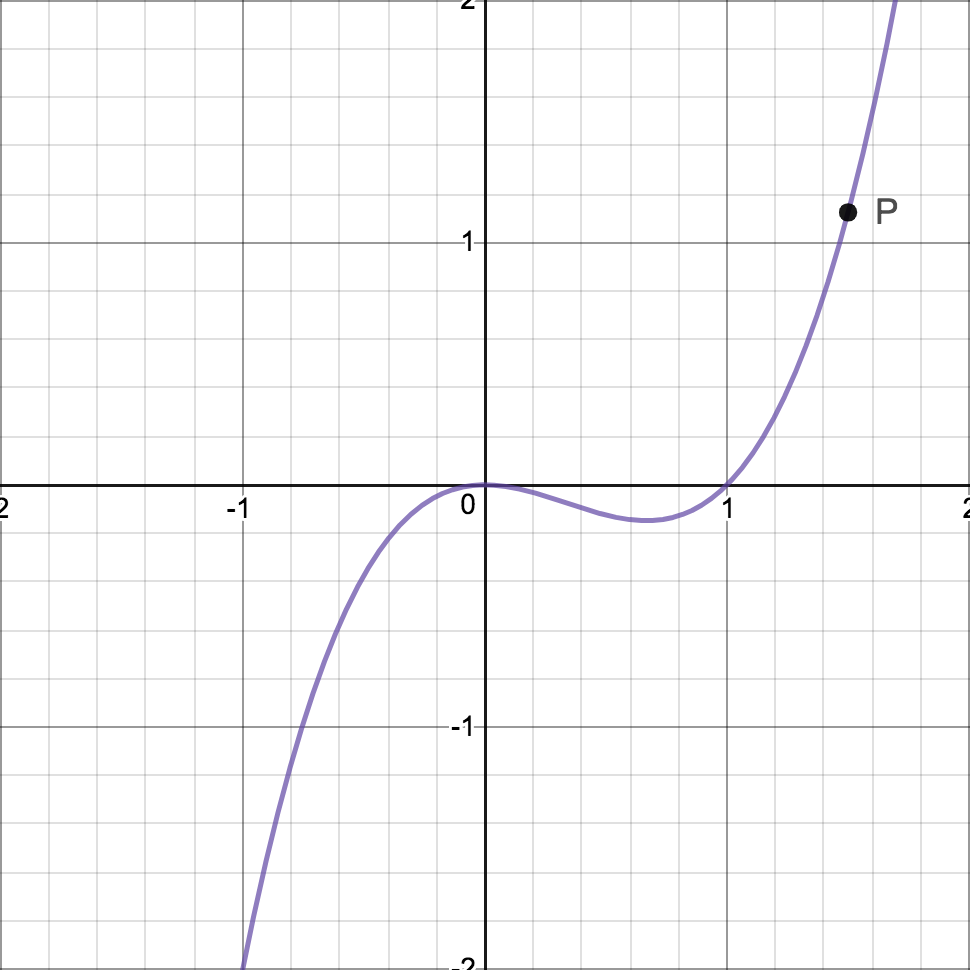
\includegraphics[width=0.3\textwidth]{14.png}
    \caption{Pick your favorite point $P\in V$. Plotted in Desmos.}
\end{figure}
Pick your favorite point $P\in V$. Often, we pick $P=0\in\mathbb{A}^n$. Look at the functions that kill $P$.

We have $\wp:=\{f\in\Gamma(V)\mid f(P)=0\}$. Note that $\wp$ is a prime ideal, since if $(fg)(P)=0$, then either $f(P)=0$ or $g(P)=0$. Also, $1\notin\wp$, so $\wp\subsetneq\Gamma(V)$. We can then localize at $\wp$.
\begin{definition}
    The \ita{local ring of V} is $\mathcal{O}_P(V):=\Gamma(V)_{\wp}\subseteq k(V)$.
\end{definition}
This really is a local ring, with maximal ideal
\begin{equation}
    \mathfrak{m}_P:=\left\{\frac{f}{g}\in\mathcal{O}_p(V)\middle|f(P)=0\right\}.
\end{equation}
In essence, take polynomials that don't vanish at $P$. Then you can divide by them!\\\\
\underline{Example}: In $\mathbb{A}^2$, let $V:=V(Y)$ (so this is just the $X$-axis). Then
\begin{align*}
    \Gamma(V)&=k[X,Y]/I(V(Y))\\
    &=k[X,Y]/\vbrack{Y}\\
    &\cong k[\overline{X}].
\end{align*}
\begin{figure}[H]
    \centering
    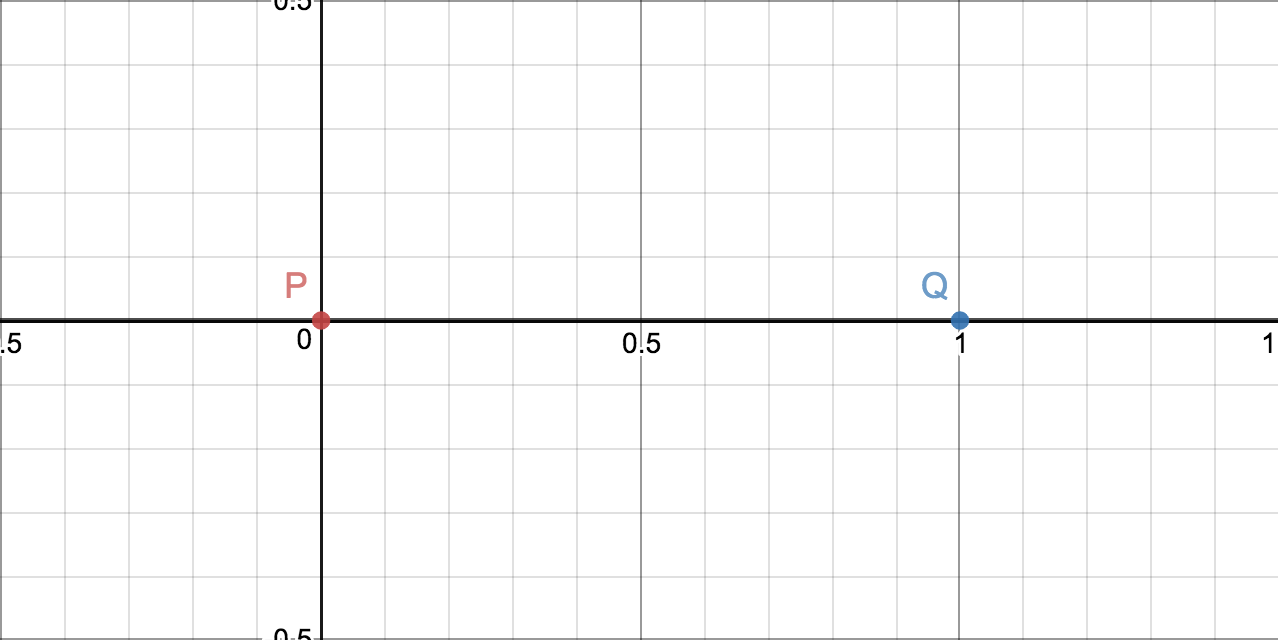
\includegraphics[width=0.5\textwidth]{15.png}
    \caption{$V(Y)$, with points $P=(0,0)$ and $Q=(1,0)$. Plotted in Desmos.}
\end{figure}
Let $P:=(0,0)$. The functions that are $0$ at $P$ are all those without a non-zero constant term:
\[\mathcal{O}_P(V)=k[\overline{X}]_{\vbrack{\overline{X}}}=\left\{\frac{f(\overline{X})}{g(\overline{X})}\,\middle|\,g(0)\neq0\right\}.\]
For another example, take $Q:=(1,0)$. Now the functions that vanish at $0$ are multiples of $X-1$, so 
\[\mathcal{O}_Q(V)=k[\overline{X}]_{\vbrack{\overline{X}}}=\left\{\frac{f(\overline{X})}{g(\overline{X})}\,\middle|\,g(0)\neq1\right\}.\]
Note that $\mathcal{O}_P(V)\cong\mathcal{O}_Q(V)$ via the map $\overline{X}\mapsto\overline{X}-1$.

Intuitively, the local appearance of $V$ at $(0,0)$ is the same as at $(1,0)$ (and in fact would be the same at any $(a,0)$). 
\begin{definition}
    Any $f\in k(V)$ can be written as $f=\frac{g}{h}$, where $g,h\in\Gamma(V)$. However, $g$ and $h$ are not necessarily unique.
    \begin{itemize}
        \item  For $P\in V$, we say $f$ is \ita{defined at P} if $f=\frac{g}{h}$ for some $g,h\in\Gamma(V)$ with $h(P)\neq0$.
        \item We say $f(P):=\frac{g(P)}{h(P)}$ is the \ita{value of f at P}. This is independent of the choice of $g$ and $h$.
        \item For $f\in k(V)$, we call the set of points in $V$ where $f$ is undefined the \ita{pole set of f}.
    \end{itemize}
\end{definition}
This should all make intuitive sense: just think of rational functions being undefined where the denominator is zero!

Here are some connections to other definitions:
\begin{enumerate}
    \item Our local ring $\mathcal{O}_P(V)$ is exactly the set $\{f\in k(V)\mid f\text{ is defined at }P\}$.
    \item Its maximal ideal is $\mathfrak{m}_P(V)=\{f\in\mathcal{O}_P(V)\mid f(P)=0\}$.
\end{enumerate}
\underline{Example}: In $\mathbb{A}^2$, take $V:=V(Y-X^2)$. Then 
\[\Gamma(V)=k[X,Y]/\vbrack{Y-X^2}\cong k[\overline{X}],\]
and $I(V)=\vbrack{Y-X^2}$. So 
\[K(V)=\left\{\frac{F(\overline{X},\overline{Y})}{G(\overline{X},\overline{Y})}\middle|G(x,y)\notin I(V)\right\}.\]
Let $f:=\frac{\overline{Y}}{\overline{X}}\in k(V)$. It looks like the pole set for $f$ might be $\{(0,0)\}$. But we can write
\[f=\frac{\overline{X}^2}{\overline{X}}=\overline{X},\]
which has no poles! So the pole set of $f$ is just $\emptyset$.

Let $f:=\frac{\overline{Y}}{\overline{X}^2-1}\in k(V)$. It looks like the pole set is $\{(\pm1,1)\}$. In fact it is, and we can prove this: Suppose $f$ is (sneakily) defined at, say $(1,1)$. Then $f=\frac{g}{h}$ for some $g,h\in\Gamma(V)$ such that $h(1,1)\neq0$. Since $f=\frac{\overline{Y}}{\overline{X}^2-1}$, $\overline{Y}h=(\overline{X}^2-1)g$. Plug in $(1,1)$ to both sides:
\[1\cdot h(1,1)=0\implies h(1,1)=0,\]
which is a contradiction. So the pole set is $\{(\pm1,1)\}$.
\section{27 February}
\subsection{Miniquiz}
For $V:=\mathbb{A}^2$, what is $\Gamma(V)$?
\subsection{Refresher of Definitions}
Let $V$ be a variety.
\begin{itemize}
    \item coordinate ring: $\Gamma(V):=k[X_1,\dotsc,X_n]/I(V)$
    \item quotient field (field of fractions): $k(V)=\left\{\frac{f}{g}\,\middle|\,f,g\in\Gamma(V),g\neq0\right\}$
    \item prime ideal for $P\in V$: $\wp=\{f\in\Gamma(V)\mid f(p)=0\}$
    \item local ring of $V$ at $P$: $\mathcal{O}_P(V):=\Gamma(V)_{\wp}=\left\{\frac{f}{g}\,\middle|\,f,g\in\Gamma(V),g(P)\neq0\right\}$
\end{itemize}
\subsection{Quantifying the Ideal-Variety Correspondence}
\begin{theorem}[Continuum Theorem]
    Let $k$ be algebraically closed, $n\geq2$, and $F\in k[X_1,\dotsc,X_n]$ be a non-constant polynomial. Then $V(F)$ is infinite.
\end{theorem}
\begin{proof}
    Since $k$ is algebraically closed, $k$ is infinite. Since $F$ is non-constant, at least one $X_i$ appears in $F$, say $X_1$. Then for every $(a_2,\dotsc,a_n)\in k^{n-1}$, the polynomial $F[X_1,a_2,\dotsc,a_n]\in k[X_1]$ has at least \ita{one} root, since $k$ is algebraically closed. Let $a_1$ be this root. Then $(a_1,\dotsc,a_n)\in V(F)$. Since there were infinitely many choices for $(a_2,\dotsc,a_n)$ to start with, $V(F)$ must be infinite.
\end{proof}
\begin{remark}
   Do not confuse this for the Continuum Hypothesis!
\end{remark}
\begin{lemma}[Gauss' Lemma]
    If $F(X)\in\z[X]$ is irreducible over $\z$, then it is also irreducible over $\q$.
    
    More generally, let $R$ be a unique factorization domain with quotient field $Q$. If $F(X)\in R[X]$ is irreducible over $R$, then $F(X)\in Q[X]$ is irreducible over $Q$.
\end{lemma}
\begin{proof}
    Ask Big Joe.
\end{proof}
\begin{theorem}[Finite Intersection Theorem]
    Let $F,G\in k[X,Y]$ have no common factors. Then the intersection $V(F,G)=V(F)\cap V(G)$ is finite.
\end{theorem}
\begin{proof}
    Factor $F$ and $G$ into distinct irreducibles,
    \[F=\prod\limits_{i=1}^rF_i^{a_i},\qquad G=\prod\limits_{j=1}^sG_j^{b_j}.\]
    Decompose $V(F,G)$ into
    \[V(F_1\dotsm F_r,G_1\dotsm G_s)=\bigcup\limits_{i,j=1}^{r,s}V(F_i,G_j).\]
    So it suffices to show that each $V(F_i,G_j)$ is finite. By relabeling $F_i$ and $G_j$ as $\Tilde{F}$ and $\Tilde{G}$, we may assume that both of them are irreducible. Consider $\Tilde{F},\Tilde{G}\in k[Y][X]$. By Gauss' Lemma (take $R:=k[Y]$ and $Q=k(Y)$), $\Tilde{F}$ and $\Tilde{G}$ are still irreducible in $k(Y)[X]$. Since $k(Y)$ is a field, $k(Y)[X]$ is a PID, and so we can talk about $\gcd$. Now $\gcd(\Tilde{F},\Tilde{G})=1$, so there exists $N,M\in k(Y)[X]$ such that
    \[N\Tilde{F}+M\Tilde{G}=1.\]
    Find a common denominator $D\in k[Y]$ such that $DN,DM\in k[Y][X]$. Then
    \[DN\Tilde{F}+DM\Tilde{G}=D.\]
    The LHS of the above expression is an element of $k[X,Y]$, but the RHS belongs to $k[Y]$ only. Now suppose $(x_0,y_0)\in V(F,G)$. So $F(x_0,y_0)=G(x_0,y_0)=0$. Then $D(y_0)=0$. Since $D\in k[Y]$, it has only finitely many roots, and so there are only finitely many $y_0$ available. Similarly, there are only finitely many $x_0$ available, so there are only finitely many points $(x_0,y_0)\in V(F,G)$.
\end{proof}
\begin{theorem}[Dimension Theorem]
    Let $k$ be algebraically closed, and let $J\subseteq k[X_1,\dotsc,X_n]$ be an ideal. Then $V(J)$ is finite if and only if $\mathrm{dim}_k(k[X_1,\dotsc,X_n]/J)$ is finite. Moreover, if $V(J)=\{P_1,\dotsc,P_r\}$, then
    \begin{equation}
        k[X_1,\dotsc,X_n]/J\cong\prod\limits_{i=1}^r\mathcal{O}_{P_i}(\mathbb{A}^n)/\vbrack{J}.
    \end{equation}
\end{theorem}
\begin{remark}
   This should be plausible: the bigger $J$ is, the smaller $V(J)$ is, and the smaller $k[X_1,\dotsc,X_n]/J$ is. In fact, the proof shows that $|V(J)|\leq\dim_k(k[X_1,\dotsc,X_n]/J)$.
\end{remark}
\underline{Example}: Let $J:=\vbrack{X^2-X,Y^2-Y}\subset k[X,Y]$. Then in $k[X,Y]/J$, we have $\overline{X}^2=\overline{X}$ and $\overline{Y}^2=\overline{Y}$, so every polynomial reduces to $a+b\overline{X}+c\overline{Y}+d\overline{X}\,\overline{Y}$. This has dimension 4 over $k$. What is $V(J)$?
\begin{figure}[H]
    \centering
    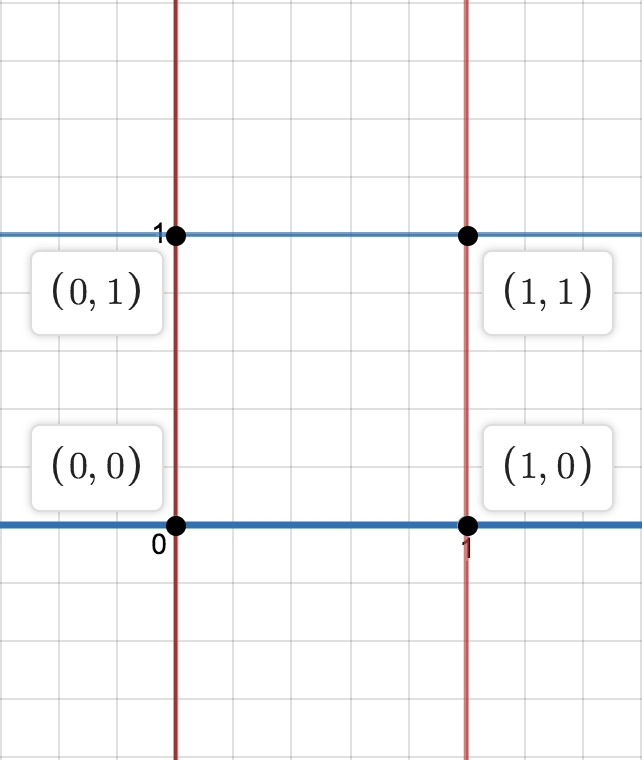
\includegraphics[width=0.3\textwidth]{16.png}
    \caption{$V(J)=\{(0,0),(1,0),(0,1),(1,1)\}$ . Plotted in Desmos.}
\end{figure}
Consider $P=(0,0)$. Then $\Gamma(\mathbb{A}^2)=k[X,Y]$, and
\[\mathcal{O}_{(0,0)}(\mathbb{A}^2)=k[X,Y]_{\vbrack{X,Y}}=\left\{\frac{f}{g}\,\middle|\,g(0,0)\neq0\right\},\]
and
\[\mathcal{O}_{(0,0)}(\mathbb{A}^2)/\vbrack{J}=\left\{\frac{a+b\overline{X}+c\overline{Y}+d\overline{X}\,\overline{Y}}{e+f\overline{X}+d\overline{Y}+f\overline{X}\,\overline{Y}}\,\middle|\,e\neq0\right\}.\]
However, we have set $\overline{X}^2=\overline{X}$, so $\overline{X}(\overline{X}-1)=0$. But in the local ring, $\overline{X}-1$ is a unit, so $\overline{X}=0$. Similarly, $\overline{Y}=0$, so our ring reduces to $\left\{\frac{a}{e}\,\middle|\,e\neq0\right\}\cong k$, which is one dimensional over $k$.

The other three points have similar results, so the product is isomorphic to $\mathbb{A}^4(k)$.
\begin{corollary}
    \[\mathrm{dim}_k(k[X_1,\dotsc,X_n]/J)=\sum\limits_{i=1}^r\mathrm{dim}_k[\mathcal{O}_{P_i}(\mathbb{A}^n)/\vbrack{J}].\]
\end{corollary}
\begin{corollary}
    If $V(J)=\{P\}$, then $k[X_1,\dotsc,X_n]/J\cong\mathcal{O}_P(\mathbb{A}^n)/\vbrack{J}$.
\end{corollary}
\section{05 March}
\subsection{Miniquiz}
Let $F:=Y-X^2+1$, $G:=X^2+Y^2-1$. Find $V(F,G)$ in $\mathbb{A}^2(\real)$.
\subsection{From Last Time}
\begin{theorem}[Dimension Theorem]
    Let $k$ be algebraically closed, and let $J\subseteq k[X_1,\dotsc,X_n]$ be an ideal. Then $V(J)$ is finite if and only if $\dim_k(k[X_1,\dotsc,X_n]/J)$ is finite. If $V(J)=\{P_1,\dotsc,P_r\}$, then
    \begin{equation}
        k[X_1,\dotsc,X_n]/J\cong\prod\limits_{i=1}^r\mathcal{O}_{P_i}(\mathbb{A}^n)/\vbrack{J}.
    \end{equation}
\end{theorem}
\begin{corollary}
    If $F,G\in k[X,Y]$ have no common factors, then
    \begin{equation}
        k[X,Y]/\vbrack{F,G}\cong\prod\limits_{P\in V(F,G)}\mathcal{O}_P(\mathbb{A}^2)/\vbrack{F,G}.
    \end{equation}
\end{corollary}
\subsection{Example}
Let's unpack what (24) means with an illuminating example. In $\mathbb{A}^2(k)$, let $F:=Y$, $G:=Y^2-(X^3+X^2)$, $J:=\vbrack{F,G}$. Note that $J=\vbrack{Y,X^3+X^2}$.
\begin{figure}[H]
    \centering
    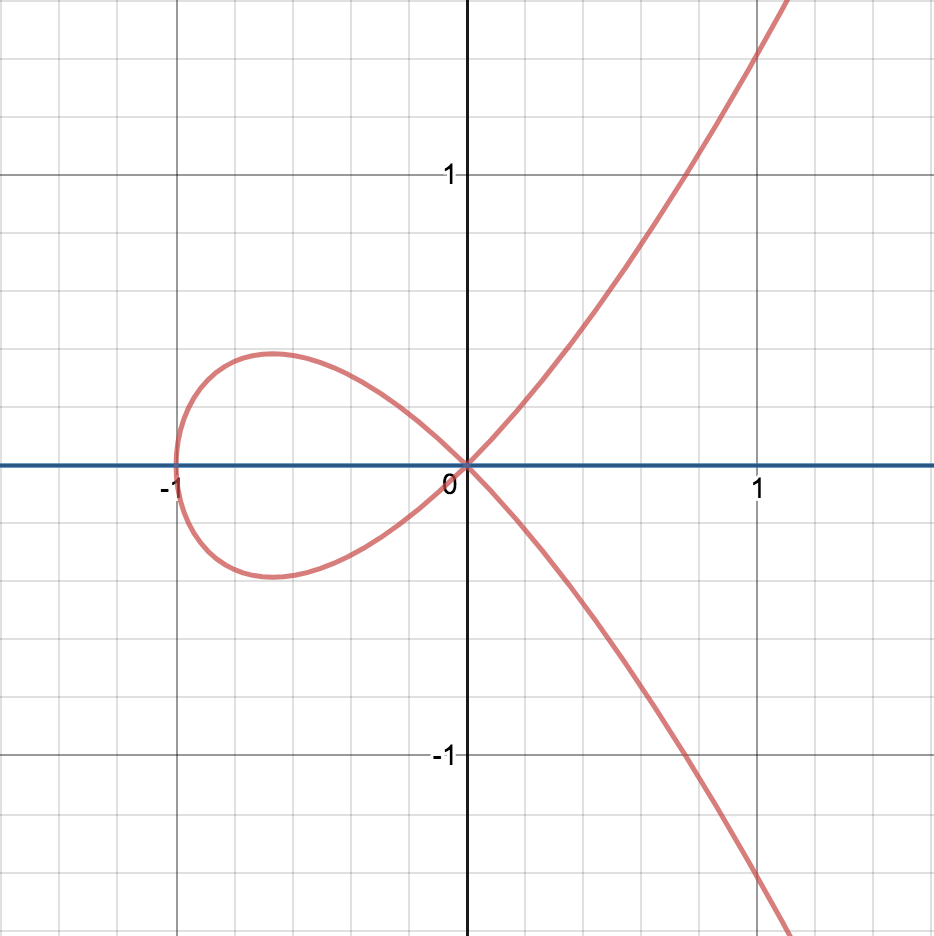
\includegraphics[width=0.3\textwidth]{17.png}
    \caption{$V(F)$ and $V(G)$ as plotted in $\mathbb{A}^2(\real)$. Note that this is only a heuristic picture, as $k$ must be algebraically closed, while $\real$ is not. Plotted in Desmos.}
\end{figure}
Consider the LHS first: 
\begin{align*}
    k[X,Y]/J&=k[X]/\vbrack{X^3+X^2}\\
    &=\{a+b\overline{X}+c\overline{X}^2\mid a,b,c\in k\}.
\end{align*}
This has $\dim_k=3$. This wasn't too bad, but the RHS is much more intriguing:
\begin{align*}
    RHS&=\prod\limits_{P\in V(F,G)}\mathcal{O}_P(\mathbb{A}^2)/\vbrack{F,G}\\
    &=\mathcal{O}_{(0,0)}(\mathbb{A}^2)/\vbrack{F,G}\times \mathcal{O}_{(-1,0)}(\mathbb{A}^2)/\vbrack{F,G}
\end{align*}
Let's examine each piece individually.
\begin{itemize}
    \item For the piece corresponding to $(-1,0)$, we have
    \begin{align*}
        \mathcal{O}_{(-1,0)}(\mathbb{A}^2)/\vbrack{F,G}&=k[X,Y]_{\vbrack{X+1,Y}}/\vbrack{J}\\
        &=\left\{\frac{a+b\overline{X}+c\overline{X}^2}{d+e\overline{X}+f\overline{X}^2}\,\middle|\,a,\dotsc,f\in k\text{ and the denominator does not vanish }\right\}
    \end{align*}
    Since $\overline{X}^3+\overline{X}^2=0$, we have $\overline{X}^2(\overline{X}+1)=0$. Note that $\overline{X}^2$ is a unit, since $\overline{X}^2\notin\vbrack{X+1,Y}$. Then $\overline{X}+1=0\Rightarrow\overline{X}=-1$. This gives us
    \begin{align*}
        \mathcal{O}_{(-1,0)}(\mathbb{A}^2)/\vbrack{F,G}&=\left\{\frac{a}{d}\,\middle|\,d\neq0\right\}\\
        &=k.
    \end{align*}
    $k$ has $\dim_k=1$.
    \item For the piece corresponding to $(0,0)$, we have
    \begin{align*}
        \mathcal{O}_{(0,0)}(\mathbb{A}^2)/\vbrack{F,G}&=k[X,Y]_{\vbrack{X,Y}}/\vbrack{J}\\
        &=\left\{\frac{a+b\overline{X}+c\overline{X}^2}{d+e\overline{X}+f\overline{X}^2}\,\middle|\,a,\dotsc,f\in k\text{ and }d\neq0\right\}
    \end{align*}
    This time, $\overline{X}+1$ is a unit, since $\overline{X}+1\notin\vbrack{X,Y}$. Thus $\overline{X}^2=0$, and we have
    \[\mathcal{O}_{(0,0)}(\mathbb{A}^2)/\vbrack{F,G}=\left\{\frac{a+b\overline{X}}{d+e\overline{X}}\,\middle|\,a,b,c,d,e\in k,d\neq0\right\}.\]
    \begin{claim}
        We can eliminate the denominators.
    \end{claim}
    \begin{proof}
        Given $d,e\in k$ such that $d\neq0$, we can solve 
        \[\frac{1}{d+e\overline{X}}=\alpha+\beta\overline{X}\]
        by solving 
        \begin{align*}
            1&=(\alpha+\beta\overline{X})(d+e\overline{X})\\
            &=\alpha d+(\alpha e+\beta d)\overline{X}+\beta e\overline{X}^2\\
            &=\alpha d+(\alpha e+\beta d)\overline{X}\because\overline{X}^2=0.
        \end{align*}
        Plugging in $\overline{X}=0$, we find $\alpha d=1\Rightarrow\alpha=\dfrac{1}{d}$. This is valid because $d\neq0$. Solving for $\beta$ gives
        \begin{align*}
            \alpha e+\beta d&=0\\
            \Rightarrow\frac{e}{d}+\beta d&=0\\
            \Rightarrow \beta&=-\frac{e}{d^2}.
        \end{align*}
        Again, this is valid since $d\neq0$ and $k$ is a field, so it has no non-trivial nilpotents.
    \end{proof}
    So 
    \[\mathcal{O}_{(0,0)}(\mathbb{A}^2)/\vbrack{F,G}=\{a+b\overline{X}\mid a,b\in k\}.\]
    This has $\dim_k=2$.
\end{itemize}
Hence we have the dimensions adding up to 3 as expected!
\subsection{The DVR}
\underline{Motivation:} Many of our local rings $\mathcal{O}_P(V)$ turn out to be DVR's. And no, that does not mean digital video recorder!
\begin{theorem}
    Let $R$ be a ring. Then the following are equivalent, and define $R$ being a $\mathrm{Discrete}$ $\mathrm{Valuation}$ $\mathrm{Ring}$.
    \begin{enumerate}
        \item $R$ is a local PID that is not a field.
        \item $R$ is a noetherian local integral domain in which the maximum ideal is principal, and $R$ is not a field.
    \end{enumerate}
\end{theorem}
\begin{remark}
   There are many different but equivalent definitions of DVR's. Clearly we have $1\Rightarrow2$, since PID $\Rightarrow$ noetherian. We will prove that $2\Rightarrow1$ later.
   
   Also, we don't want $R$ to be a field since fields only have $\{0\}$ as their maximal ideal, and that's just boring!
\end{remark}
\underline{Examples}:
\begin{itemize}
    \item From Homework 5, $R=\left\{\dfrac{a}{b}\,\middle|\,b\equiv0\text{ (mod) }2\right\}$ is a DVR, with unique maximal ideal $\mathfrak{m}=\vbrack{2}$.
    \item In general, $\z_{\vbrack{p}}$ works, with $\mathfrak{m}=\vbrack{p}$.
    \item Similarly, $k[X]_{\vbrack{X}}=\left\{\frac{F(X)}{G(X)}\,\middle|\,G(0)\neq0\right\}$ is a DVR, with $\mathfrak{m}=\left\{\frac{F(X)}{G(X)}\,\middle|\,F(0)=0\right\}$.
    \item Another example from Homework 5 is the formal power series!
    \[k[[X]]:=\left\{\sum\limits_{n=0}^{\infty}a_nX^n\,\middle|\,a_n\in k\right\},\]
    with $\mathfrak{m}=\vbrack{X}$.
\end{itemize}
\underline{Aside}: Why is 3 prime? It's because any factorization of 3 includes a unit.
\begin{definition}
    $r\in R$ is \ita{irreducible} if $r$ is not a unit itself and any factorization $r=ab$ means either $a$ or $b$ is a unit.
\end{definition}
There's an important property of DVR's that is sometimes taken as a definition.
\begin{definition}
    There exists an irreducible $t\in R$ such that every non-zero $r\in R$ satisfies $r=ut^n$ for a unique unit $u\in R$ and natural number $n\in\n$. $t$ is called the \ita{uniformizing parameter}.
\end{definition}
\underline{Examples}:
\begin{itemize}
    \item In $\z_{\vbrack{p}}$, $t=p$.
    \item In both $k[X]_{\vbrack{X}}$ and $k[[X]]$, $t=X$.
\end{itemize}
Let's actually prove that this is a property of a DVR.
\begin{proof}
    Using definition 2), since $R$ is not a field, $\{0\}$ cannot be the maximal idea. Then $\mathfrak{m}=\vbrack{t}$ for some $t\in R\setminus\{0\}$. We claim that $t$ is irreducible. Otherwise, $t=ab$ for some $a,b\in R^{\times}$ (units of $R$). Look at $a$: $t\in\vbrack{a}$, so $\mathfrak{m}\subseteq\vbrack{a}\subsetneq R$, so $m=\vbrack{a}$ by maximality. Then $a=tc$ for some $c\in R$, and so
    \begin{align*}
        a&=abc\\
        1&=bc.
    \end{align*}
    (Note that the cancellation law used to get to the 2nd line above is OK in a domain.) Hence $b$ is a unit, which is a contradiction because $b$ was assumed to be a non-unit. Hence $t$ is irreducible. \checkmark
    
    Let $r\in R\setminus\{0\}$. If $r$ is a unit, then $r=rt^0$, as desired. Otherwise, $r\in\mathfrak{m}=\vbrack{t}$. Let $n\geq1$ be maximal such that $t^n\mid r$, and let $r:=ut^n$. Note that $u$ is a unit, otherwise $t^{n+1}\mid r$, contradicting the maximality of $n$. \checkmark
    
    To show uniqueness, suppose $r=ut^n=vt^m$ for units $u$ and $v$. By factoring $t's$ (assuming $n\leq m$), we have $u=vt^{m-n}$. Since $v$ is a unit, $t^{m-n}=v^{-1}u$, which is a contradiction to $t$ being a non-unit. So $m=n\Rightarrow u=v$. \checkmark
\end{proof}
\section{06 March}
\subsection{Miniquiz}
In the local ring $k[[X]]$, $1+X\notin\mathfrak{m}=\vbrack{X}$, so $1+X$ should be a unit. What is its inverse?
\subsection{DVR's (continued)}
Recall that the following are equivalent and characterize a DVR:
\begin{enumerate}
    \item (strong) a local PID that is not a field
    \item (weak) a local noetherian domain that is not a field, where $\mathfrak{m}$ is principal
\end{enumerate}
We had an important property that also characterized a DVR: there exists an irreducible $t\in R$ such that every $r\in R\setminus\{0\}$ is uniquely written as $r=ut^n$ for some unit $u$ and $n\in\n$. $t$ is called the \ita{uniformizing parameter}, and this was proven using the weak characterization of DVR's.

Finally, let's prove that the weak characterization does imply the strong one.
\begin{proof}
    Let $J\subseteq R$ be an ideal. Since $R$ is noetherian,
    \begin{align*}
        J&=\vbrack{r_1,\dotsc,r_s}\\
        &=\vbrack{u_1t^{n_1},\dotsc,u_st^{n_s}}\\
        &=\vbrack{t^{n_1},\dotsc,t^{n_s}}\\
        &=\vbrack{t^n},
    \end{align*}
    where $n:=\min\limits_{1\leq i\leq s}n_i$. So $R$ is a PID.
\end{proof}
Let's look at a new characterization of a DVR.
\begin{definition}
    Let $Q$ be the field of fractions of $R$. Then there is a surjective function $\mathrm{ord}:Q\twoheadrightarrow\z\cup\{\infty\}$, called the \ita{order} or \ita{valuation} satisfying
    \begin{enumerate}
        \item $\mathrm{ord}(0):=\infty$
        \item $\mathrm{ord}(q_1q_2)=\mathrm{ord}(q_1)+\mathrm{ord}(q_2)$
        \item $\mathrm{ord}(q_1+q_2)\geq\min\{\mathrm{ord}(q_1),\mathrm{ord}(q_2)\}$.
    \end{enumerate}
    Moreover, $R=\{q\in Q\mid\mathrm{ord}(q)\geq0\}$.
\end{definition}
\begin{proof}
    (Sketch) Take $\mathrm{ord}(0):=\infty$ by definition, and note that every $q\in Q$ can be written $\frac{a}{b}$, where $a,b\in R$ and $a=ut^n$ and $b=vt^m$ for units $a,b$. Then $q$ can be rewritten as $q=uv^{-1}t^{n-m}$. We can then write $q=wt^r$ for a unit $w$ and $r\in\z$ (possibly negative). Set $\mathrm{ord}(q):=r$.
\end{proof}
Roughly speaking, $\mathrm{ord}$ counts how many $t$'s ``divides'' $q$.\\\\
\underline{Example}: Let $R:=\z_{\vbrack{3}}$, with maximal ideal $\mathfrak{m}=\vbrack{3}$, and ring of fractions $\q$. Recall that 
\[\z_{\vbrack{3}}=\left\{\frac{a}{b}\in\q\,\middle|\,3\nmid b\right\}=\{q\in\q\mid\mathrm{ord}(q)\geq0\}.\]
\begin{itemize}
    \item $\mathrm{ord}(54)=3$, because $54=2\times 3^3$.
    \item $\mathrm{ord}\left(\frac{5}{18}\right)=2$, because $\frac{1}{18}=2^{-1}\times3^{-2}$.
    \item $\mathrm{ord}\left(\frac{17}{100}\right)=0$, because $\gcd(3,17)=\gcd(3,100)=1$.
\end{itemize}
\underline{Visualizing a DVR}:
\begin{align*}
    &R=\vbrack{1}=\vbrack{u}\text{ for any unit }u\\
    &\cup\\
    &\mathfrak{m}=\vbrack{t}=\vbrack{ut}\text{ for any unit }u\\
    &\cup\\
    &\mathfrak{m}^2\\
    &\cup\\
    &\vdots
\end{align*}
This shows that DVR's are \ita{not} artinian, but powers of the maximal ideal are the only ideals. $\mathrm{ord}$ records where you are in this hierarchy. 
\subsection{Multiplicity in the Affine Plane}
Recall that the \ita{tangent line} to a curve $y=f(x)$ at a point $(x_0,y_0)$ is given by the point-slope formula
\begin{equation*}
    \begin{split}
        &y-y_0=f'(x_0)(x-x_0)\\
        \Rightarrow&1(y-y_0)-f'(x_0)(x-x_0)=0
    \end{split}
\end{equation*}
Let $F(x,y):=y-f(x)$. Then $\frac{\partial F}{\partial x}=-f'(x)$ and $\frac{\partial F}{\partial y}=1$, so the equation of the tangent line can be rewritten as 
\begin{equation}
    \left(\left.\frac{\partial F}{\partial x}\right|_P\right)(x-x_0)+\left(\left.\frac{\partial F}{\partial y}\right|_P\right)(y-y_0)=0
\end{equation}
where $P:=(x_0,y_0)$.\\\\
Moving up a dimension, recall that the \ita{tangent plane} to a surface $F(x,y,z)=0$ in $\real^3$ at $P=(x_0,y_0,z_0)$ is given by 
\begin{equation}
    \left(\left.\nabla F\right|_P\right)\cdot(\mathbf{x}-P)=0
\end{equation}
where $\mathbf{x}=(x,y,z)\in\real^3$.
\begin{definition}
    For $F\in k[X_1,\dotsc,X_n]$, $P=(a_1,\dotsc,a_n)\in\mathbb{A}^n(k)$, define the \ita{tangent hyperplane to F at P} as
    \begin{equation}
        \left\{(x_1,\dotsc,x_n)\in\mathbb{A}^n(k)\,\middle|\,\sum\limits_{i=1}^n\left(\left.\frac{\partial F}{\partial x_i}\right|_P\right)(x_i-a_i)=0\right\}
    \end{equation}
\end{definition}
This usually works nicely.
\begin{remark}
   Let us address the elephant in the room: how in the world are we able to take \ita{derivatives} in any field?! Since we are working with polynomials, we are able to get away with this by defining the derivative as a formal operation.
\end{remark}
\underline{Example}:  Let $F(X,Y)=Y^2-X^3-X^2$. Then $F_X=-3X^2-2X$ and $F_Y=2Y$.
\begin{figure}[H]
    \centering
    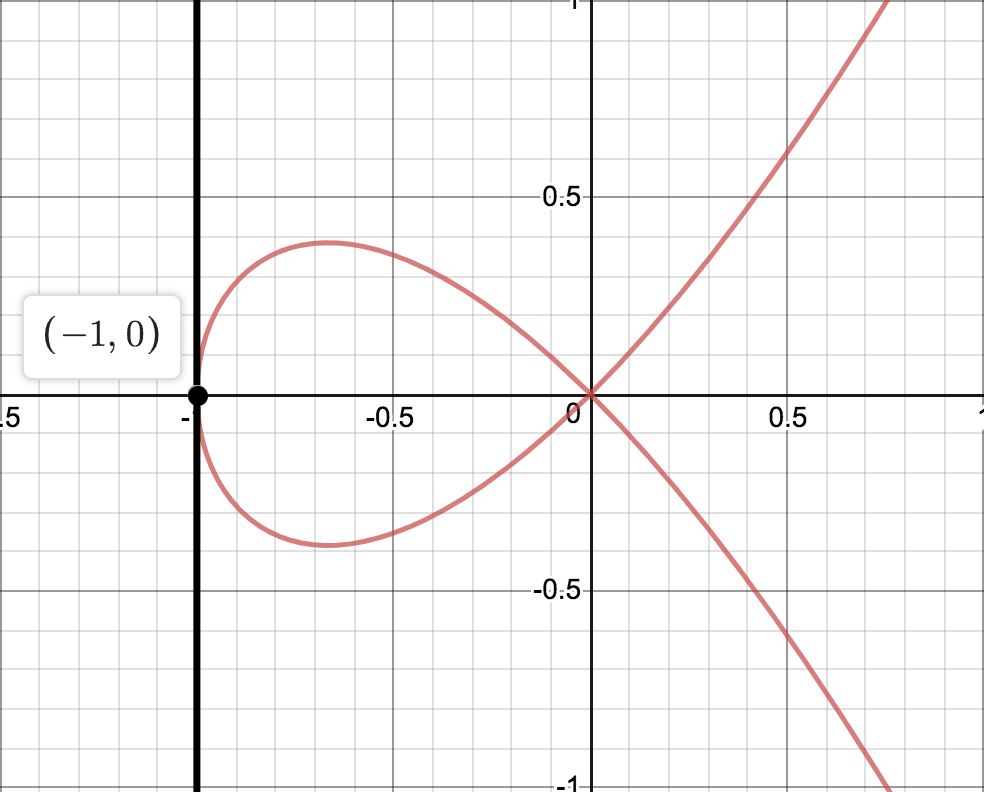
\includegraphics[width=0.3\textwidth]{18.png}
    \caption{$V(F)$, as plotted in $\mathbb{A}^2(\real)$, and the tangent line $X=-1$ to $V(F)$ at $Q=(-1,0)$.}
\end{figure}
Let $Q:=(-1,0)$, then $F_X(Q)=-1$ and $F_Y(Q)=0$. Plug $Q$ into (27) to find the tangent line at $Q$:
\[-1(X+1)+0(Y-0)=0\Rightarrow X+1=0\Rightarrow X=-1.\]
Let $P:=(0,0)$, then $F_X(P)=F_Y(P)=0$. Plugging this into (27) yields the ever-useful $0=0$. So $F$ has no single well-defined tangent line at $P$.
\begin{definition}
    Beware: some of these terms are not the best.
    \begin{itemize}
        \item $P$ is a \ita{simple} (also $\ita{smooth}$ or $\ita{non-singular}$) point of $F$ if at least one $F_{x_i}(P)\neq0$. Then there is a well-defined tangent hyperplane in $\mathbb{A}^n$ at $P$.
        \item $P$ is a \ita{multiple} (also \ita{singular} or \ita{critical}) point on $F$ if $\nabla F\mid_P=(0,\dotsc,0)$.
        \item $F$ is \ita{non-singular} if every point on $F$ is simple. $F$ is \ita{singular} if any point on $F$ is multiple.
    \end{itemize}
\end{definition}
\begin{remark}
   We will specialize to $P=(0,0)$ in $\mathbb{A}^2$. We choose $\mathbb{A}^2$ to make things easy to draw, and we choose the origin for simplicity. We can always translate $F$ to study another point, so sticking with the origin is OK.
\end{remark}
To examine the behavior of $F$ around $(0,0)$, write $F=F_m+F_{m+1}+\dotsb+F_n$, where each $F_i$ is a homogenous polynomial of degree $i$ and $F_m\neq0$. Note that $m\geq1$, since $(0,0)$ is a point on $V(F)$.\\\\
\underline{Example}: Using $F(X,Y)=Y^2-X^3-X^2=(Y^2-X^2)-X^3$, we have $F_2=Y^2-X^2$ and $F_3=-X^3$.\\\\
\underline{Intuition}: The \ita{local} behavior of $F$ around $(0,0)$ is determined by the lowest powers $F_m$, since higher terms decrease more rapidly.\\\\
\underline{Example}: Using the same $F$ as before, we have $F\sim Y^2-X^2=(Y-X)(Y+X)$. 
\begin{figure}[H]
    \centering
    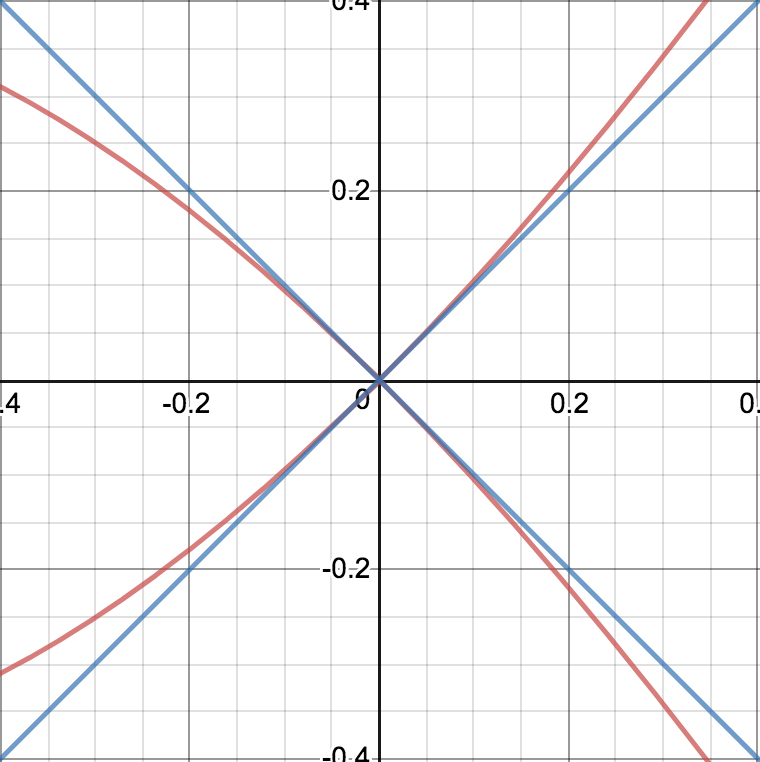
\includegraphics[width=0.3\textwidth]{19.png}
    \caption{$V(F)$ looks like $V((Y-X)(Y+X))$ near $(0,0)$. Plotted in Desmos.}
\end{figure}
\begin{definition}
    The \ita{multiplicity} of $P$ on $F$ is $m_P(F):=m$.
\end{definition}
\underline{Example}: For our recurring example, $m_P(F)=2$. 

To examine what $m_Q(F)$ is, we would need to translate $X$ and $Y$ so that $(-1,0)$ lands on the origin. Let's do exactly this: 
\[F(X,Y)\mapsto \Tilde{F}(X,Y)=Y^2-(X-1)^3-(X-1)^2\]
\begin{figure}[H]
    \centering
    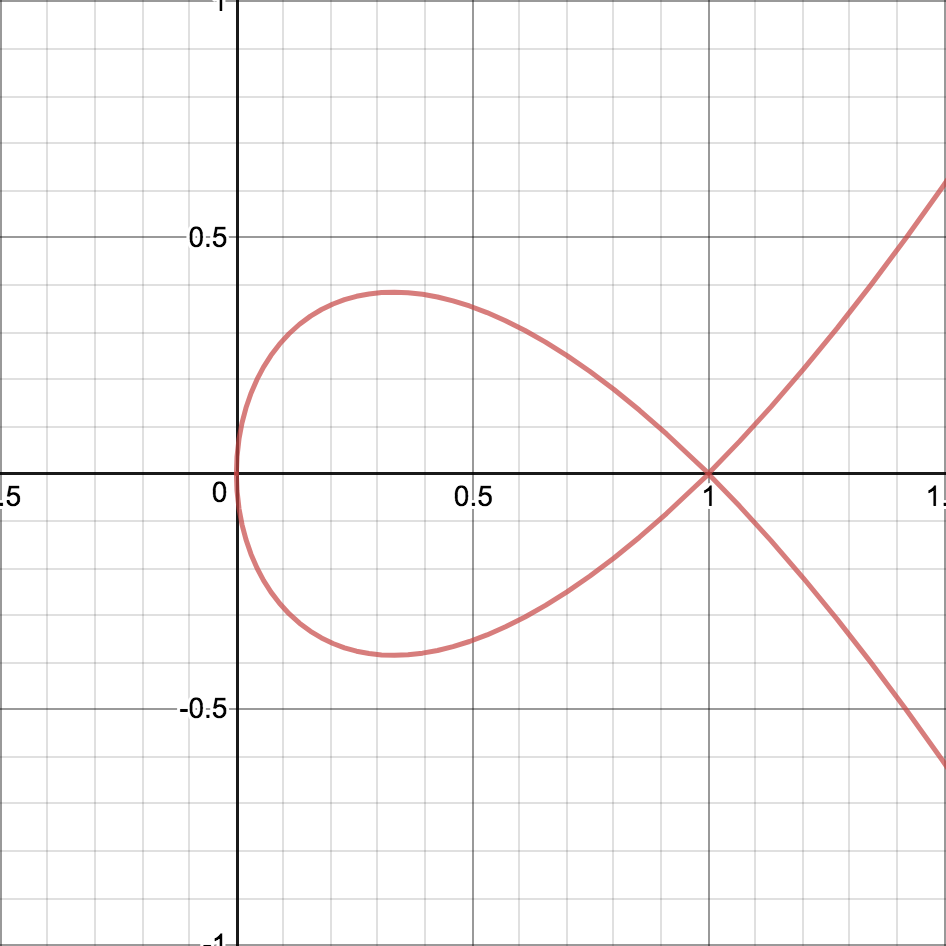
\includegraphics[width=0.3\textwidth]{20.png}
    \caption{$V(\Tilde{F})$}
\end{figure}
\section{11 March}
\subsection{Miniquiz}
Find the tangent line to $F:=X^4-2Y^3+3X^2Y+X^2-4XY+2X-Y$ at $P:=(0,0)$. Also find the multiplicity $m_P(F)$.
\subsection{From Last Time}
Recall the following definitions:
\begin{itemize}
    \item \underline{Single point}: at least one $F_{X_i}(P)\neq0$.
    \item \underline{Multiple point}: all $F_{X_i}(P)=0$.
    \item \underline{Tangent hyperplane}: at $P:=(a_1,\dotsc,a_n)$: $\sum\limits_{i=1}^nF_{X_i}(P)(X_i-a_i)=0$.
    \item \underline{Multiplicity}: $m_P(F):=m$, where $F=F_m+F_{m+1}+\dotsb+F_t$, $F_m\not\equiv0$, $i:=\deg F_i$.
\end{itemize}
Some notes on multiplicity:
\begin{enumerate}
    \item Because non-zero derivatives at $(0,0)$ come from terms of degree 1, $P=(0,0)$ is a simple point if and only if $m_P(F)=1$, and it is a multiple if and only if $m_P(F)>1$. And $P$ is not on $F$ if and only if $m_P(F)=0$.
    \item $m_P(F)$ depends only on those components of $F$ that go through $P$. That is, if $F=GH$ with $G(P)=0\neq H(P)$, then $m_P(F)=m_P(G)$; we can disregard $H$.
\end{enumerate}
For example, consider $F=(Y-X^2)(X-1)$. It clearly consists of a part that vanishes at $(0,0)$ and one that does not.
\begin{figure}[H]
    \centering
    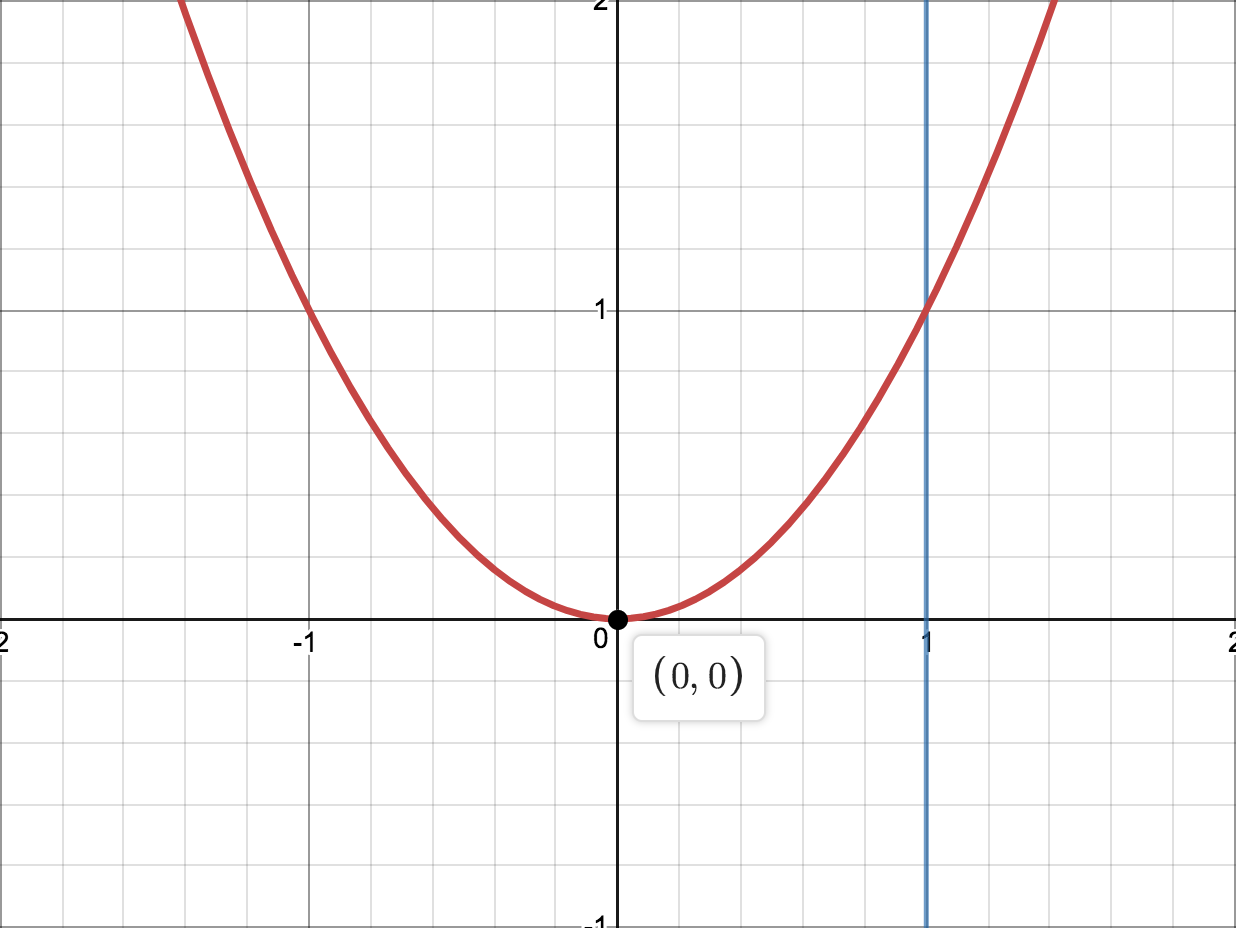
\includegraphics[width=0.3\textwidth]{21.png}
    \caption{$V(F)$. Plotted in Desmos.}
\end{figure}
We can even prove the second point rigorously: assuming $P=(0,0)$, suppose $H(P)=\alpha\neq0$. Let $m:=m_P(G)$, then $G=G_m+G_{m+1}+\dotsb+G_t$. Then $F=GH=G_m\alpha+\text{ higher degree terms }$, so $m_P(F)=m=m_P(G)$. $\qed$
\subsection{The DMT}
\begin{figure}[H]
    \centering
    
\includegraphics[width=0.5\textwidth]{22.jpg}
    \caption{This section is best enjoyed while listening to this remix: \url{https://www.youtube.com/watch?v=FPs3EeRyL9Y}}
\end{figure}
Assume $k$ is algebraically closed. Let $P$ be a point on the irreducible curve $F$. Then $V:=V(F)$ is a variety with coordinate ring $\Gamma(V)=k[X,Y]/\vbrack{F}$. We have the local ring $\mathcal{O}_P:=\Gamma(V)_{\wp}=\left\{\frac{g}{h}\,\middle|\,g,h\in\Gamma(V),h(P)\neq0\right\}$, with unique maximal ideal $\mathfrak{m}_P(V)=\left\{\frac{g}{h}\,\middle|\,g(P)\neq0\right\}=\vbrack{\wp}$.

Let's consider powers $\mathfrak{m}_P^n(F)$ (multiply $\mathfrak{m}_P(F)$ by itself $n$ times as an ideal). These are ideals, so they are $k$-vector spaces. Higher powers are smaller: $\mathfrak{m}_P^{n+1}(F)\subseteq \mathfrak{m}_P^n(F)$. We can mod out (as vector spaces) to form the quotient space $\mathfrak{m}_P^n(F)/\mathfrak{m}_P^{n+1}(F)$.
\begin{theorem}[Dimension and Multiplicity Theorem (DMT)]
    For all $n\geq m_P(F)$ (multiplicity!), we have
    \begin{equation}
        \dim_k[\mathfrak{m}_P^n(F)/\mathfrak{m}_P^{n+1}(F)]=m_P(F).
    \end{equation}
\end{theorem}
\begin{remark}
   \begin{enumerate}
       \item We have been subtly abusing notation this whole time, writing $\mathfrak{m}_P(F)$ when we really mean $\mathfrak{m}_P(V(F))$.
       \item We'll actually prove this for $n\geq m_P(F)-1$.
       \item What about for $n<m_P(F)$? Then
       \begin{equation}
           \dim_k[\mathfrak{m}_P^n(F)/\mathfrak{m}_P^{n+1}(F)]=n+1.
       \end{equation}
       This is homework.
   \end{enumerate}
\end{remark}
Some tools for the proof:
\begin{itemize}
    \item \textbf{Pole proposition}: Let $V$ be a variety. Let $P=(a_1,\dotsc,a_n)\in V$. Then $\mathcal{O}_P(V)$ is a local noetherian domain with $\mathfrak{m}_P(V)=\vbrack{\overline{X}_1-a_1,\dotsc,\overline{X}_n-a_n}$. Indeed, $\mathcal{O}_P(V)$ is the localization of $\Gamma(V)$ at $\vbrack{\overline{X}_1-a_1,\dotsc,\overline{X}_n-a_n}$. 
    \item \textbf{Local corollary}: For any $n\geq0$, we have
    \begin{equation}
        \mathcal{O}/\mathfrak{m}\cong k[X,y]/\vbrack{\vbrack{F}+\vbrack{X,Y}^n}.
    \end{equation}
    \item \textbf{Triangle lemma}: $\dim_k(k[X,Y]/\vbrack{X,Y}^d)=\frac{1}{2}d(d+1)$.
\end{itemize}
We will only proof the triangle lemma:
\begin{proof}
    When we mod out by $\vbrack{X,Y}^d$, we are left with polynomials of degree $d-1$ or less. This has basis
    \[\begin{tabular}{ c c c c c c c c c }
    \empty & \empty & \empty & \empty & $1$ & \empty & \empty & \empty & \empty \\
    \empty & \empty & \empty & $X$ & \empty & $Y$ & \empty & \empty & \empty \\
    \empty & \empty & $X^2$ & \empty & $XY$ & \empty & $Y^2$ & \empty & \empty \\
    \empty & $X^3$ & \empty & $X^2Y$ & \empty & $XY^2$ & \empty & $Y^3$ & \empty \\
    \empty & \empty & \empty & \empty & $\vdots$ & \empty & \empty & \empty & \empty \\
    $X^{d-1}$ & \empty & $X^{d-2}Y$ & \empty & $\dots$ & \empty & $XY^{d-2}$ & \empty & $Y^{d-1}$
    \end{tabular}\]
    $k[X,Y]/\vbrack{X,Y}^d$ has a triangular basis. So the dimension is 
    \[1+2+3+\dotsb+d=\frac{1}{2}d(d+1).\]
\end{proof}
Finally, the proof of the DMT!
\begin{proof}
    To simplify notation, set $m:=m_P(F)$ (multiplicity), $\mathcal{O}:=\mathcal{O}_P(V)$, $\mathfrak{m}:=\mathfrak{m}_P(F)$. We may assume that $P=(0,0)$.
    
    By the pole proposition, we have $\mathfrak{m}=\vbrack{\overline{X},\overline{Y}}\subsetneq\mathcal{O}$. Recall that
    \[\mathcal{O}\supsetneq\mathfrak{m}\supseteq\mathfrak{m}^2\supseteq\mathfrak{m}^3\supseteq\dotsb\supseteq\mathfrak{m}^n\supseteq\mathfrak{m}^{n+1}\supseteq\dotsb\]
    We have a \underline{key claim}: for all $n\geq m$, we have $\dim_k(\mathcal{O}/\mathfrak{m})=mn+s$ for some constant $s$.
    
    Assuming this claim holds, we simply apply it to obtain
    \begin{align*}
        \dim_k(\mathfrak{m}^n/\mathfrak{m}^{n+1})&=\dim_k(\mathcal{O}/\mathfrak{m}^{n+1})-\dim_k(\mathcal{O}/\mathfrak{m}^n)\\
        &=m(n+1)+s-(mn+s)\\
        &=m. \checkmark
    \end{align*}
\end{proof}
Now let's prove the key claim.
\begin{proof}
    By the local corollary, we must measure the dimension of $k[X,Y]/\vbrack{\vbrack{F}+\vbrack{X,Y}^n}$. Make an exact sequence:
    \[\{0\}\xlongrightarrow{}k[X,Y]/\vbrack{X,Y}^{n-m}\xlongrightarrow{\psi}k[X,Y]/\vbrack{X,Y}^n\xlongrightarrow{\pi}k[X,Y]/\vbrack{\vbrack{F}+\vbrack{X,Y}^n}\xlongrightarrow{}\{0\}.\]
    \begin{itemize}
        \item To show that $\psi$ is well-defined, decompose $F=F_m+F_{m+1}+\dotsb+F_t$. Then if $G\in\vbrack{X-Y}^{n-m}$, \ita{i.e.}, $\overline{G}=\overline{0}$ in $k[X,Y]/\vbrack{X,Y}^{n-m}$, we have $FG=(F_m+F_{m+1}+\dotsb+F_t)G\in\vbrack{X,Y}^n$. So $\psi(\overline{G})=\overline{0}$. \checkmark
        \item $\psi$ is injective, because if $FG\in\vbrack{X,Y}^n$, then $G\in\vbrack{X,Y}^{n-m}$, so $\overline{G}=\overline{0}$ in $k[X,Y]/\vbrack{X,Y}^{n-m}$. \checkmark
        \item To show exactness in the middle, note that
        \begin{align*}
            \mathrm{Im}\psi&=(\text{all multiples of }F)+\vbrack{X,Y}^n\\
        &=\vbrack{\vbrack{F}+\vbrack{X,Y}^n}\\
        &=\ker\pi. \checkmark
        \end{align*}
        \item $\pi$ is automatically surjective. \checkmark
    \end{itemize}
    By the Exact Dimension Theorem, 
    \begin{align*}
        \dim_k(k[X,Y]/\vbrack{\vbrack{F}+\vbrack{X,Y}^n})&=\dim_k(k[X,Y]/\vbrack{X,Y}^n)-\dim_k(k[X,Y]/\vbrack{X,Y}^{n-m})\\
        &=\frac{1}{2}n(n+1)-\frac{1}{2}(n-m)(n-m+1)\\
        &=nm+\frac{1}{2}m(1-m)\\
        &=nm+s. \checkmark
    \end{align*}
\end{proof}
\section{13 March}
\subsection{Miniquiz}
Let $0\xlongrightarrow{}A\xlongrightarrow{}B\xlongrightarrow{}C\xlongrightarrow{}0$ be an exact sequence of vector spaces with $\dim B=15$ and $\dim C=5$. What is $\dim A$?
\subsection{More on the DMT}
Recall the \underline{DMT}: For all $n\geq m_P(F)$, we have
\[\dim_k\left[\mathfrak{m}_P^n(F)/\mathfrak{m}_P^{n+1}(F)\right].\]
Let's focus on a couple of examples to get an idea of what this theorem really says:
\begin{itemize}
    \item $F:=Y-X^2$, $P:=(0,0)$. $m_P(F)=1$ (the lowest power is $Y^1$). $\Gamma(V(F))=k[X,Y]/\vbrack{Y-X^2}\cong k[X]$, and $\mathcal{O}=\left\{\frac{g}{h}\,\middle|\,g,h\in k[X],h(0)\neq0\right\}$. Take $\mathfrak{m}^0=\mathcal{O}$. This isn't too unreasonable: think about how $\vbrack{2}^0=\vbrack{2^0}=\vbrack{1}$. Then $\mathfrak{m}^1=\left\{\frac{g}{h}\,\middle|\,g(0)=0\right\}=\vbrack{X}$, and so $\dim(\mathfrak{m}^0/\mathfrak{m}^1)=1$. Note that
    \[\mathfrak{m}^0=\left\{\frac{g_0+g_1X+g_2X^2+\dotsb+g_nX^n}{h_0+h_1X+h_2X^2+\dotsb+h_mX^m}\,\middle|\,n,m\in\z^+,h_0\neq0\right\}\]
    \[\mathfrak{m}^1=\left\{\frac{g_1X+g_2X^2+\dotsb+g_nX^n}{h_0+h_1X+h_2X^2+\dotsb+h_mX^m}\,\middle|\,n,m\in\z^+,h_0\neq0\right\}\]
    When working over mod $\mathfrak{m}$, we get
    \[\left\{\frac{g_0}{h_0}\,\middle|\,h_0\neq0\right\}=k.\]
    So $\mathfrak{m}^0/\mathfrak{m}^1$ is spanned by 1. Moving up, we have
    \[\mathfrak{m}^2=\left\{\frac{g_2X^2+g_3X^3+\dotsb}{h}\right\}=\vbrack{X^2}.\]
    Working over mod $\mathfrak{m}^2$, we have
    \[\mathfrak{m}^1/\mathfrak{m}^2=\left\{\frac{g_1X}{h}\right\}=\text{span}_k\{X\}.\]
    Thus $\dim_k(\mathfrak{m}^1/\mathfrak{m}^2)=1$.
    
    This becomes easier to see if we just ignore the dimensions:
    \begin{align*}
        \mathfrak{m}^0&=\{g_0+g_1X+g_2X^2+g_3X^3+\dotsb\},\dim_k=1\\
        \mathfrak{m}^1&=\{g_1X+g_2X^2+g_3X^3+\dotsb\},\dim_k=1\\
        \mathfrak{m}^2&=\{g_2X^2+g_3X^3+\dotsb\},\dim_k=1\\
        \mathfrak{m}^3&=\{g_3X^3+\dotsb\},\dim_k=1.
    \end{align*}
    $\mathfrak{m}^0/\mathfrak{m}^1$ is spanned by 1, $\mathfrak{m}^1/\mathfrak{m}^2$ is spanned by $X$, $\mathfrak{m}^2/\mathfrak{m}^3$ is spanned by $X^2$.
    
    Since $m_P(F)=1$, each $\mathfrak{m}^n/\mathfrak{m}^{n+1}$ is just a $m_P(F)$-dimensional (one-dimensional) vector space.
    \item Let $F:=Y^2-X^3-X^2$, $P:=(0,0)$. Then $m_P(F)=2$, and 
    \[\Gamma(V(F))=k[X,Y]/\vbrack{Y^2-X^3-X^2}\cong k[X]\oplus k[X]Y,\]
    and
    \[\mathcal{O}=\left\{\frac{g}{h}\,\middle|\,g,h\in\Gamma,h(0,0)\neq0\right\}.\]
    Again, the denominators are not important, so we will ignore them.
    \begin{align*}
        \mathfrak{m}^0&=\{g_1(X)+g_2(X)Y\}=\mathrm{span}_k\{1\}\\
        \mathfrak{m}^1&=\{g_1(X)+g_2(X)Y\mid g_1(0)=0\}=\mathrm{span}_k\{X,Y\}\\
        \mathfrak{m}^2&=\{g_2(X)X^2+g_3(X)X^3+\dotsb+h(X)Y\mid h(0)=0\}=\mathrm{span}_k\{X^2,XY\}\\
        \mathfrak{m}^n&=\{g_1(X)+g_2(X)Y\mid\text{ lowest powers on }g_1\text{ and }g_2\text{ are }n\text{ and }n-1\text{, respectively }\}
    \end{align*}
\end{itemize}
Notice the difference between these two examples:
\begin{itemize}
    \item The long term dimension kicked in at $\mathfrak{m}^0/\mathfrak{m}^1$, since $m_P(F)=1$.
    \item The long term dimension kicked in at $\mathfrak{m}^1/\mathfrak{m}^2$, since $m_P(F)=2$.
\end{itemize}
\subsection{Intersection Numbers}
\underline{Motivating Example}: $Y-X^2$ has a double root at 0. So we want to say that $Y=X^2$ and $Y=0$ intersect ``twice'' there. 
\begin{figure}[H]
    \centering
    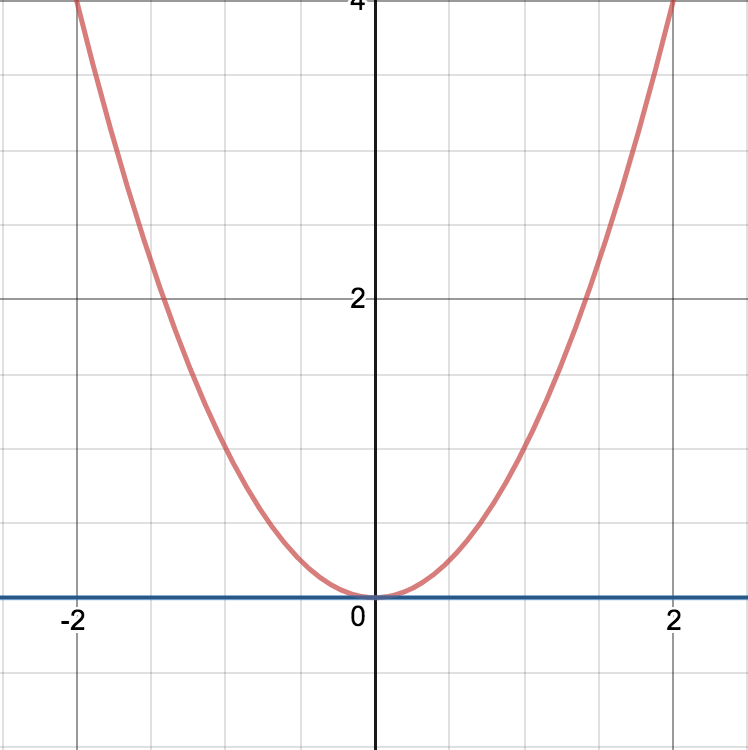
\includegraphics[width=0.3\textwidth]{23.png}
    \caption{$Y-X^2=0$ and $Y=0$ intersect ``twice'' at $(0,0)$. Plotted in Desmos.}
\end{figure}
More precisely, the intersection number of $F:=Y-X^2$ and $G:=Y$ at $P=(0,0)$ should be 2.
\begin{definition}
    Let $F,G\in k[X,Y]$ be curves in $\mathbb{A}^2$. We define the \ita{intersection number} of $F$ and $G$ at $P\in\mathbb{A}^2$ to be
    \begin{equation}
        I_P(F,G):=\dim_k\left[\mathcal{O}_P(\mathbb{A}^2)/\vbrack{F,G}\right].
    \end{equation}
\end{definition}
\begin{remark}
   Fulton uses the notation $I(P,F\cap G)$ instead.
\end{remark}
Recall that $I(\mathbb{A}^2)=\{0\}$, so $\Gamma(\mathbb{A}^2)=k[X,Y]/\{0\}\cong k[X,Y]$. For $P\in\mathbb{A}^2$, $\wp=\{f\in\Gamma(V)\mid f(P)=0\}$, and
\[\mathcal{O}_P(\mathbb{A}^2)=\Gamma(\mathbb{A}^2)_{\wp}=\left\{\frac{f}{g}\,\middle|\,f,g\in k[X,Y],g(P)\neq0\right\}.\]
This definition is not very enlightening at first, but we will explore this further.\\\\
\underline{Example}: Let $F:=Y$, $G:=Y-X^n$, $P:=(0,0)$. Then $\vbrack{F,G}=\vbrack{Y,Y-X^n}=\vbrack{Y,X^n}$, and 
\[\mathcal{O}_P(\mathbb{A}^2)/\vbrack{F,G}=\left\{\frac{f}{g}\,\middle|\,f,g\in k[X],g(0)\neq0,X^n=0\right\}.\]
Hence we have made $X$ nilpotent!

We claim that we can eliminate denominators: if $g(0)\neq0$, then we can solve
\[\frac{1}{g_0+g_1X+\dotsb+g_{n-1}X^{n-1}}=a_0+a_1X+\dotsb+a_{n-1}X^{n-1}.\]
Then $a_0g_0=1$, and since $g_0\neq0$, $a_0=\frac{1}{g_0}$. Moving onto $a_1$, we have $g_0a_1+a_0g_1=0$, and we can solve for $a_1$. Thus we can continue in this fashion to solve for each $a_i$.

So every element of $\mathcal{O}_P(\mathbb{A}^n)/\vbrack{F,G}$ can be written as $f_0+f_1X+\dotsb+f_{n-1}X^{n-1}$, and so it has basis $\{1,X,\dotsc,X^{n-1}\}$. Hence $\dim_k=n$.
\section{18 March}
\subsection{Miniquiz}
Find $I(F,G)$ for $F:=X$, $G:=Y^2$, $P:=(0,0)$.
\subsection{Intersection Numbers (cont'd)}
Recall the \underline{Dimension Theorem}: $V(J)$ is finite if and only if $\dim_k(k[X,Y]/J)$ is finite, and
\[k[X,Y]/J\cong\prod\limits_{P\in V(J)}\mathcal{O}_P(\mathbb{A}^2)/\vbrack{J}.\]
\begin{definition}
    $F,G\in k[X,Y]$ are curves in $\mathbb{A}^2$. Let $P\in\mathbb{A}^2$. Define the \ita{intersection number}
    \[I(F,G):=\dim_k[\mathcal{O}_P(\mathbb{A}^2)/\vbrack{F,G}].\]
\end{definition}
\underline{Example}: We calculated $I(Y-X^n,Y)=n$.

Intersection numbers needn't be that hard. Let's make it easier (and more intuitive).
\subsection{Properties of Intersection Numbers}
\begin{enumerate}
    \item \underline{Positivity}: $I(F,G)\in\n\cup\{+\infty\}$, $+\infty$ means countable infinity.
    \begin{proof}
        This is just the dimension of a vector space!
    \end{proof}
    \item $I(F,G)=0$ if and only if $P\notin F\cup G$.
    \begin{proof}
        Suppose $P$ is not on $F$, meaning $F(P)\neq0$. Then in the local ring $\mathcal{O}_P(\mathbb{A}^2)=\left\{\frac{f}{g}\,\middle|\,f,g\in k[X,Y],g(P)\neq0\right\}$, $F$ is a denominator and so it is a unit. Then $\vbrack{F,G}$ is just the whole ring, so $\mathcal{O}_P(\mathbb{A}^2)/\vbrack{F,G}=\{0\}$. Then $I(F,G)=\dim_k\{0\}=0$. Siilarly, if $P$ is not on $G$, $I(F,G)=0$.
        
        Conversely, if $I(F,G)=0$, then $\dim_k[\mathcal{O}_P(\mathbb{A}^2)/\vbrack{F,G}]=0$. Hence $\vbrack{F,G}=\mathcal{O}_P(\mathbb{A}^2)$, so $\vbrack{F,G}$ contains a unit. Say $aF+bG$ is a unit, which means $(aF+bG)(P)\neq0$. So $F(P)\neq0$ or $G(P)\neq0$, and $P\notin F\cap G$.
    \end{proof}
    \item \underline{Symmetry}: $I(F,G)=I(G,F)$.
    \begin{proof}
        $\vbrack{F,G}=\vbrack{G,F}$, so done!
    \end{proof}
    \item \underline{Locality}: $I(F,G)$ depends only on the components of $F$ and $G$ containing $P$.
    \begin{proof}
        Suppose $F=AH$ with $A(P)\neq0$. Then within $\mathcal{O}_P(\mathbb{A}^2)$, the ideal $\vbrack{F,G}=\vbrack{AH,G}=\vbrack{H,G}$, because $A$ is a unit. So we can factor out and discard all components of $F$ and $G$ that don't contain $D$.
    \end{proof}
    \item \underline{Gaussian Reduction}: (less intuitive, but useful algebraically) For any polynomial $A\in k[X,Y]$, we have $I(F,G)=I(F,G+AF)$. 
    \begin{proof}
        \begin{align*}
            \vbrack{F,G+AF}&=\vbrack{F}+\vbrack{G+AF}\\
            &=\vbrack{F}+\vbrack{G}+\vbrack{AF}\\
            &=\vbrack{F}+\vbrack{G}\\
            &=\vbrack{F,G}.
        \end{align*}
    \end{proof}
    \item \underline{Finiteness}: $I(F,G)=\infty$ if and only if $F$ and $G$ have a common irreducible component containing $P$. 
    \begin{proof}
        ($\Leftarrow$) Suppose $F$ and $G$ have a common irreducible component $H$ containing $P$. Then $H\mid F$ and $H\mid G$, and so $\vbrack{F,G}\subseteq\vbrack{H}$. By the continuum theorem, $|V(H)|=\infty$, so by the dimension theorem, $\dim_k(k[X,Y]/\vbrack{H})=\infty$. Then
        \begin{align*}
            I(F,G)&=\dim_k[\mathcal{O}_P(\mathbb{A}^2)/\vbrack{F,G}]\\
            &\geq\dim_k[\mathcal{O}_P(\mathbb{A}^2)/\vbrack{H}]\\
            &\geq\dim_k(k[X,Y]/\vbrack{H})\\
            &\geq\infty.
        \end{align*}
    \end{proof}
    ($\Rightarrow$) Suppose $F$ and $G$ have no common component containing $P$. By locality, we can discard any components of $F$ and $G$ containing $P$, so we can assume that $F$ and $G$ have no common component at all. Then the Finite Intersection Theorem says that $V(F,G)=V(F)\cap V(G)$ is finite. By the dimension theorem, $\dim_k(k[X,Y]/\vbrack{F,G})$ is finite, and
    \[k[X,Y]/\vbrack{F,G}\cong\prod\limits_{P_i\in V(F,G)}\mathcal{O}_{P_i}(\mathbb{A}^2)/\vbrack{F,G}.\]
    So each $\mathcal{O}_{P_i}(\mathbb{A}^2)/\vbrack{F,G}$ is finite-dimensional. Our $P$ is one of those $P_i$'s where $P_i\in V(F,G)$, so $I(F,G)=\dim_k[\mathcal{O}_P(\mathbb{A}^2)/\vbrack{F,G}]$ is finite.
\end{enumerate}
\underline{Notation}: Let $F$ be irreducible. If $P$ is a simple point on $F$, then by the Simple DVR Theorem (see handout: $\mathcal{O}_P(F)$ is a DVR), we have a \ita{valuation} $\mathrm{ord}$ on $\mathcal{O}_P(F)$, defined by taking $\mathrm{ord}(ut^n):=n$, where $t$ is the uniformizing parameter. $\mathfrak{t}=\mathfrak{m}_P(F)$, and every non-zero $z\in\mathcal{O}_P(F)$ can be written as $z=ut^n$. We define $\mathrm{ord}_P^F(z):=\mathrm{ord}(z)$. 
\begin{enumerate}[resume]
    \item \underline{DVR compatibility}: Let $F$ be irreducible. If $P$ is a simple point on $F$, then $I(F,G)=\mathrm{ord}_P^F(\overline{G})$.
    \begin{proof}
        See handout.
    \end{proof}
\end{enumerate}
\underline{Example}: Let $F:=Y-X^2$, $G:=Y^2-X^3$, $P:=(0,0)$. $P$ is a simple point on $F$, but not on $G$. 
\begin{figure}[H]
    \centering
    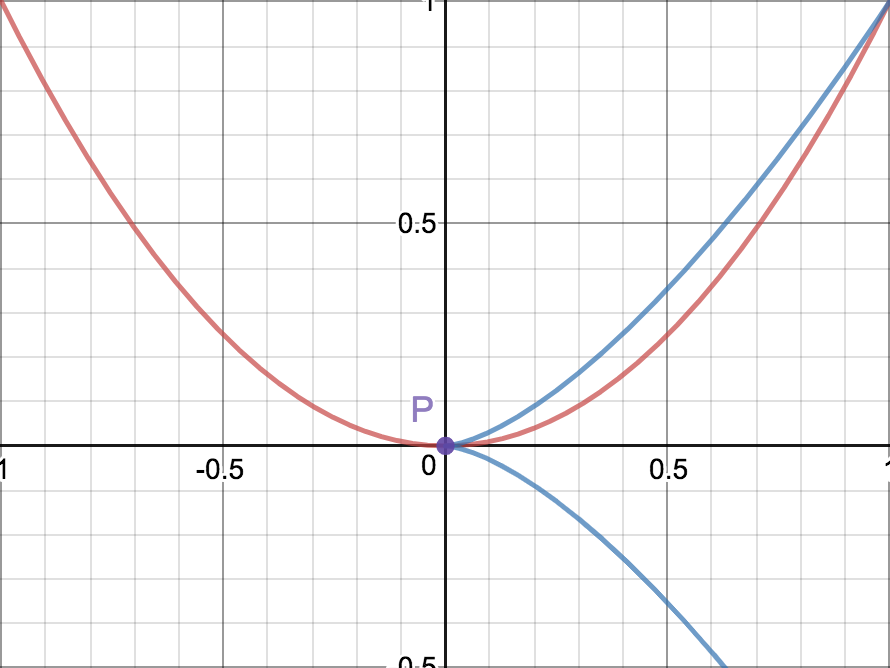
\includegraphics[width=0.4\textwidth]{24.png}
    \caption{$V(F)$, $V(G)$, and $P$. Plotted in Desmos.}
\end{figure}
Here we have $\Gamma(F)$, $\mathcal{O}_P(F)$, and $\mathfrak{m}_P(F)$.
\[\Gamma(F)=k[X,Y]/\vbrack{Y-X^2}\cong k[\overline{X}],\]
\[\mathcal{O}_P(F)=\left\{\frac{f}{g}\,\middle|\,f,g\in\Gamma(F),g(0)\neq0\right\},\]
\[\mathfrak{m}_P(F)=\left\{\frac{f}{g}\,\middle|\,f(0)=0\right\}=\vbrack{\overline{X}}.\]
Note that
\begin{align*}
    \overline{G}&=\overline{Y^2-X^3}\\
    &=\overline{X}^4-\overline{X}^3\\
    &=\overline{X}^3(\overline{X}-1).
\end{align*}
Since $\overline{X}-1$ is a unit, $\mathrm{ord}_P^F(\overline{G})=3$, so $I(F,G)=3$.
\section{25 March}
\subsection{Properties of Intersection Numbers (cont'd)}
Recall 
\[I_P(F,G):=\dim_k\left[\mathcal{O}_P(\mathbb{A}^2)/\vbrack{F,G}\right]\]
We listed the following properties:
\begin{enumerate}
    \item \underline{positivity}: $I(F,G)\geq0$
    \item \underline{positive-definite}: $I(F,G)=0$ if and only if $P\notin V(F,G)$
    \item \underline{symmetry}: $I(F,G)=I(G,F)$
    \item \underline{locality}: we may discard components of $F$ and $G$ that do not contain $P$
    \item \underline{Gaussian reduction}: $I(F,G)=I(F,G+AF)$
    \item \underline{finiteness}: $I(F,G)=\infty$ if and only if $F$ and $G$ have a common irreducible component containing $P$
    \item \underline{DVR compatibility}: if $F$ is irreducible and $P\in F$ is simple, then $I(F,G)=\mathrm{ord}_P^F(\overline{G})$
    \item \underline{weak additivity}: $I(F,GH)=I(F,G)+I(F,H)$
    
    We can build up inductively to \underline{strong additivity}: Suppose $F=\prod\limits_{i=1}^nF_i^{\alpha_i}$, $G=\prod\limits_{j=1}^mG_j^{\beta_j}$, where $F_i$ and $G_j$ are irreducibles. Then 
    \begin{equation}
        I(F,G)=\sum\limits_{i=1}^n\sum\limits_{j=1}^m\alpha_i\beta_jI(F_i,G_j).
    \end{equation}
    \begin{proof}
        (Sketch) Do some reductions:
        \begin{itemize}
            \item Use locality to discard components of $F$, $G$, and $H$ not containing $P$.
            \item Assume $H$ is irreducible.
            \item Assume $F$ and $GH$ have no common components (otherwise both sides of $I(F,GH)=I(F,G)+I(F,H)$ are $\infty$ and so we are done).
            \item Set up an exact sequence:
            \[\{0\}\xlongrightarrow{}\mathcal{O}_P(\mathbb{A}^2)/\vbrack{F,G}\xlongrightarrow{\phi:A\mapsto AH}\mathcal{O}_P(\mathbb{A}^2)/\vbrack{F,GH}\xlongrightarrow{\pi:A\mapsto A}\mathcal{O}_P(\mathbb{A}^2)/\vbrack{F,H}\xlongrightarrow{}\{0\}\]
            Check that this sequence is exact.
            \item Use Exact Dimension Theorem to get $I(F,G)+I(F,H)=I(F,GH)$.
        \end{itemize}
    \end{proof}
    \item \underline{multiplicity}: $I(F,G)\geq m_P(F)m_P(G)$, with equality holding if and only if $F$ and $G$ have no common tangent lines at $P$
    \begin{proof}
        See handout.
    \end{proof}
    \item \underline{invariance}: Let $T:\mathbb{A}^2\to\mathbb{A}^2$ be an affine transformation:
    \[T:\begin{bmatrix}
        X\\
        Y
    \end{bmatrix}\mapsto
    \begin{bmatrix}
        a & b\\
        c & d
    \end{bmatrix}
    \begin{bmatrix}
        X\\
        Y
    \end{bmatrix}
    +
    \begin{bmatrix}
        e\\
        f
    \end{bmatrix}\]
    where $ad-bc\neq0$. Then $I_{P^T}(F^T,G^T)=I_P(F,G)$.
\end{enumerate}
\subsection{Examples}
\begin{enumerate}
    \item From last time, we had $P:=(0,0)$, $F(X,Y):=Y-X^2$, $G(X,Y):=Y^2-X^3$. We found that $m_P(F)=1$, $m_P(G)=2$, and $I_P(F,G)=3$. Note that from multiplicity we have a strict inequality, since they share the same tangent line $Y=0$.
    \item Let $P:=(0,0)$ (as always), $F(X,Y):=Y^2-X^3-X^2$, and $G(X,Y):=X$.
    Then
    \begin{align*}
        I(F,G)&=I(X,Y^2-X^3-X^2)&&\text{by symmetry}\\
        &=I[X,Y^2-X^3-X^2+X(X^2+X)]&&\text{by Gaussian reduction}\\
        &=I(X,Y^2)\\
        &=2I(X,Y)&&\text{by additivity}\\
        &=2\cdot1\cdot1&&\text{by multiplicity}\\
        &=\boxed{2}
    \end{align*}
    That was quite nice!
    \item Let $P:=(0,0)$, $F(X,Y):=(X^2+Y^2)^3-4X^2Y^2$, $G(X,Y):=X^2+Y^2-2Y$, As an aside, how do we graph $F$? Use polar coordinates: $X=r\cos\theta,Y=r\sin\theta$
    \begin{align*}
        &\Rightarrow F(r,\theta)=r^6-4r^2\cos^2\theta r^2\sin^2\theta\\
        &\Rightarrow r^6=4r^4\cos^2\theta\sin^2\theta\\
        &\Rightarrow r^2=[\sin(2\theta)]^2\\
        &\Rightarrow r=\sin(2\theta).
    \end{align*}
    As for $G$, we can just complete the square:
    \begin{align*}
        G&=X^2+Y^2-2Y+1-1=0\\
        &\Rightarrow X^2+(Y-1)^2=1.
    \end{align*}
    \begin{figure}[H]
        \centering
        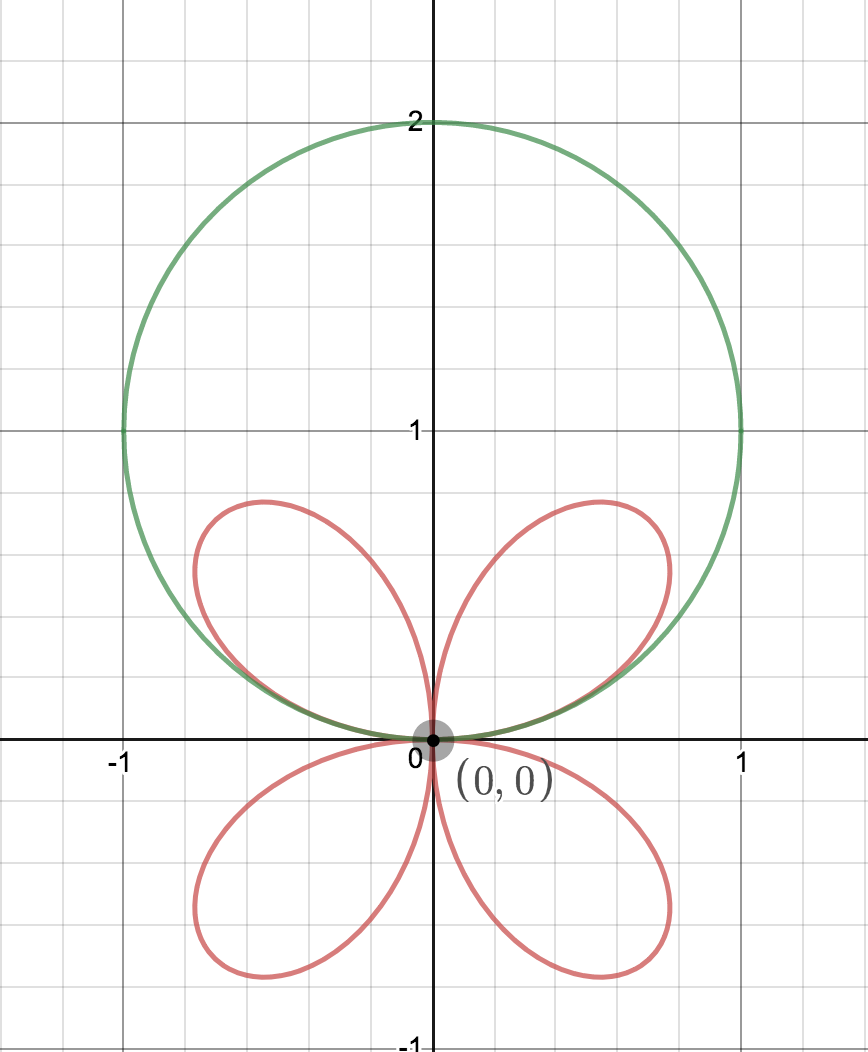
\includegraphics[width=0.5\textwidth]{25.png}
        \caption{$P$, $V(F)$, and $V(G)$ plotted in $\mathbb{A}^2(\real)$ for purposes of visualization. Plotted in Desmos.}
    \end{figure}
    By multiplicity, we know that $I(F,G)\geq4$. Let's actually compute this
    \begin{align*}
        I(F,G)&=I[(X^2+Y^2)^3-4X^2Y^2,X^2+Y^2-2Y]\\
        &=I[(2Y)^3-4X^2Y^2,X^2+Y^2-2Y]&&\text{by Gaussian reduction}\\
        &=I(8Y^3-4X^2Y^2,X^2+Y^2-2Y)\\
        &=I[4Y^2(2Y-X^2),Y^2-(2Y-X^2)]\\
        &=I[4Y^2(Y^2),X^2-Y^2-2Y]&&\text{by Gaussian reduction}\\
        &=I(Y^4,X^2+Y^2-2Y)&&\text{4 is a unit}\\
        &=4I(Y,X^2+Y^2-2Y)&&\text{by additivity}\\
        &=4I(Y,X^2)&&\text{by multiplicity}\\
        &=8I(Y,X)&&\text{by Gaussian reduction}\\
        &=\boxed{8}
    \end{align*}
\end{enumerate}
\subsection{Miniquiz}
Let $F(X,Y):=Y^2-X^3-X^2$, $G(X,Y):=Y$, $P:=(0,0)$. Find $I_P(F,G)$.
\section{27 March}
\subsection{Miniquiz}
Let $F:=X^4+Y^4+2X^2Y^2-4X^2$, $G:=X$. Find $I_{(0,0)}(F,G)$.
\subsection{Projective Space}
\underline{Goal}: Augment $\mathbb{A}^n$ with ``infinite points.'' The example to keep in mind is $k:=\real$, $n:=2$, so we're ``augmenting'' $\real^2$.\\\\
\underline{Construction}: Start with $\mathbb{A}^{n+1}$ (imagine $\real^3$ now). Exclude the origin, and impose the equivalence relation $[a_1:\cdots:a_{n+1}]\sim[\lambda a_1:\cdots:\lambda a_{n+1}]$ for $\lambda\in k^{\times}$. That is, two points are equivalent if and only if they are on the same line through the origin.
\begin{definition}
    The \ita{n-dimensional projective space over k} is 
    \begin{equation}
        \boxed{\mathbb{P}^n:=\mathbb{A}^{n+1}/\sim.}
    \end{equation}
\end{definition}
\begin{figure}[H]
        \centering
        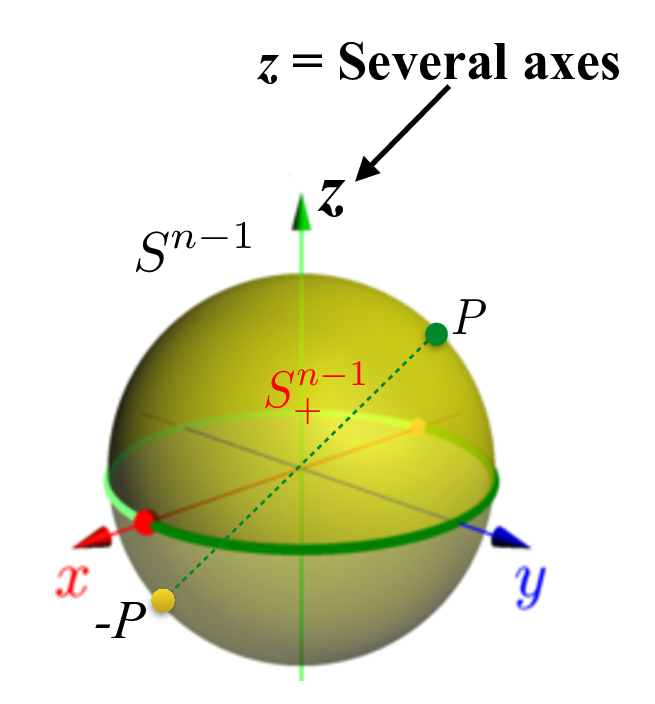
\includegraphics[width=0.3\textwidth]{53.png}
        \caption{From \url{https://www.researchgate.net/publication/287250322}.}
    \end{figure}
How to visualize $\mathbb{P}^2(\real)=\real\mathbb{P}^2$:
\begin{itemize}
    \item \underline{Round-earth model}: (geometric) (Almost) every line through $\mathbf{0}$ intersects the upper unit hemisphere in one point. So $\real\mathbb{P}^2$ is the upper unit hemisphere, except that we identify antipodal points on the equator.
    \begin{figure}[H]
        \centering
        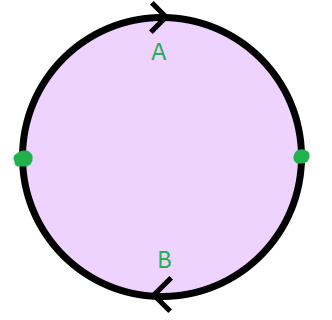
\includegraphics[width=0.3\textwidth]{28.png}
        \caption{From \url{https://math.stackexchange.com/questions/538720/}.}
    \end{figure}
    \item \underline{Flat-earth model}: (algebraic) Each line through $\mathbf{0}$ in $\real^3$ still intersects the plane $z=1$ in one point, except for the horizontal lines. So $\real\mathbb{P}^2$ is $\real^2$ augmented by one infinite point for each possible slope of a line in $\real^2$. Note that we're identifying
    \[[X:Y:Z]=\left[\frac{X}{Z}:\frac{Y}{Z}:1\right]\in\real\mathbb{P}^2,\]
    with $\left(\frac{X}{Z},\frac{Y}{Z}\right)\in\real^2$.
    \item \underline{Polyhedral model}: (surfaces) 
    \begin{figure}[H]
        \centering
        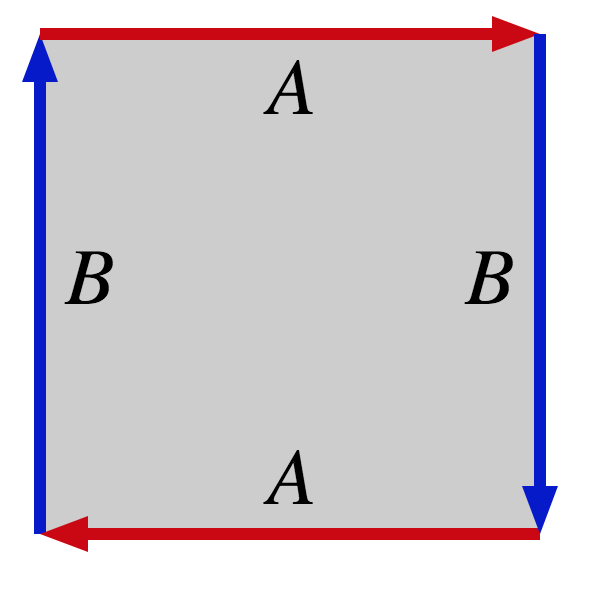
\includegraphics[width=0.3\textwidth]{27.png}
        \caption{Fundamental polygon of $\real\mathbb{P}^2$. From Wikimedia Commons.}
    \end{figure}
\end{itemize}
\subsection{Polynomials in Projective Space}
\underline{Problem}: Finding zeros of polynomials in $\mathbb{P}^n$ is not well-defined in general. For example, $F(X,Y,Z):=X^2+Y^2+Z^2-1$ has the zero $\left[\frac{3}{5}:\frac{4}{5}:0\right]$, but $\left[\frac{3}{5}:\frac{4}{5}:0\right]=[3:4:0]$, which is \ita{not} a zero of $F$.

Our solution is to restrict to \ita{homogeneous polynomials}.
\begin{definition}
    $F(X_1,\dotsc,X_{n+1})\in k[X_1,\dotsc,X_{n+1}]$ is a \ita{form of degree d} (also \ita{homogenenous of degree d}) if every monomial term of $F$ has total degree $d$.
\end{definition}
\underline{Examples}:
\begin{itemize}
    \item $F:=X^2+Y^2-37XZ$ is a form of degree $d=2$.
    \item $F:=X^2+Y^2+Z^2-1$ is not a form.
    \item $F:=X^2Y^3Z+15Y^6-23X^4Y^2$ is a form of degree $d=6$.
\end{itemize}
The zeros of a form \ita{are} well-defined:
\[F[\lambda a_1:\cdots:\lambda a_{n+1}]=\lambda^dF[a_1:\cdots:a_{n+1}].\]
So one is zero if and only if the other is.
\begin{definition}
    For a form $F\in k[X_1,\dotsc,X_{n+1}]$, we define
    \begin{equation}
        V(F):=\{[a_1:\cdots:a_{n+1}]\in\mathbb{P}^n\mid F[a_1:\cdots:a_{n+1}]=0\}.
    \end{equation}
\end{definition}
\underline{Examples}:
\begin{itemize}
    \item $F:=X^2+Y^2-Z^2$. In $\real^3$, $F=0$ is a cone. It intersects the plane $Z=1$ in a circle: $X^2+Y^2=1$.
    \begin{figure}[H]
        \centering
        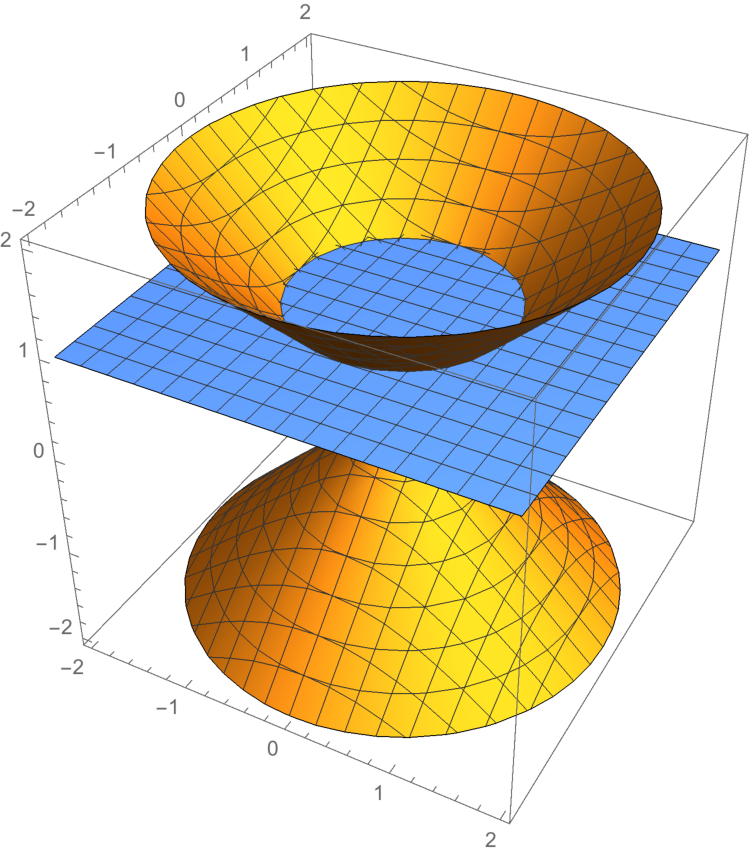
\includegraphics[width=0.3\textwidth]{26.pdf}
        \caption{$V(F)$ and $V(Z-1)$. Plotted in \ita{Mathematica}.}
    \end{figure}
    \item $F:=YZ-X^2$. At $Z=1$, we get the parabola $Y=X^2$, but we also get the infinite point $[0:1:0]$.
    \item $F:=XY-Z^2$. At $Z=1$, we get the hyperbola $XY=1$, but we also get the infinite points $[1:0:0]$ and $[0:1:0]$, closing it off into a single point. 
    \item $F:=AX+BY-CZ$, a plane in $\real^3$. At $Z=1$, we get $AX+BY=C\Rightarrow$ the line $Y=\frac{C}{B}-\frac{A}{B}X$, but we also get the infinite point $\left[1:-\frac{B}{A}:0\right]$, closing the loop.
\end{itemize}
\begin{definition}
    A \ita{graded ring} is a ring $S$ with a decomposition of additive groups $S=\bigoplus\limits_{d=0}^{\infty}S_d$, meaning each $s\in S$ can be written uniquely as $s=s_0+s_1+\dotsb+s_t$, with each $s_i\in S_i$. Moreover, degrees add under multiplication: $S_iS_j\subseteq S_{i+j}$.
\end{definition}
The sole example of a graded ring for us is
\[k[X_1,\dotsc,X_{n+1}]=\bigoplus\limits_{d=0}^{\infty}S_d,\]
where each $S_d$ consists of forms of degree $d$ and 0.\\\\
\underline{Example}: $F\in k[X,Y,Z]$
\[F(X,Y,Z)=XY^2+Y^4+2XY^2+X^2Z^2+Z^3+XY+X-7Y+8.\]
Let's try decomposing $F$ into forms:
\begin{align*}
    F&=8+(X-7Y)+(XY)+(Z^3+2XY^2)+(X^2Z^2+Y^4+XY^2Z)\\
    &=F_0+F_1+F_2+F_3+F_4.
\end{align*}
$S_d$ is a vector space over $k$. In $k[X,Y]$, we have $\dim_k(S_d)=d+1$ (see Triangle Lemma). \begin{lemma}[Pyramid Lemma]
    In $k[X,Y,Z]$, we have $\dim_k(S_d)=\binom{d+2}{2}=\frac{1}{2}(d+1)(d+2)$.
\end{lemma}
\section{08 April}
\subsection{Miniquiz}
Let $F:=Y^2Z-X^3$, $G:=Z-X^2-Y^2$. One of these has a well-defined zero set in $\real\mathbb{P}^2$. Graph the zero set (including any infinite points), and tell me why the other polynomial doesn't work.
\subsection{Homogeneous Ideals and Projective Algebraic Sets}
\begin{definition}
    Let $S=\bigoplus\limits_{d=0}^{\infty}$ be a graded ring, and let $J\subseteq S$ be an ideal. $J$ is said to be a \ita{homogeneous ideal} if $J=\bigoplus\limits_{d=0}^{\infty}$.
\end{definition}
Let $J\subseteq k[X_1,\dotsc,X_{n+1}]$ be a homogeneous ideal and $S\subseteq\mathbb{P}^n$ be any subset. We define a correspondence
\begin{align}
    V_p(J)&:=\{P\in\mathbb{P}^n\mid F(P)=0\text{ for all \ita{homogeneous}  }F\in J\}\\
    I_p(J)&:=\vbrack{F\in k[X_1,\dotsc,X_{n+1}\mid F\text{ is homogeneous and }F(P)=0\text{ for all }P\in S}.
\end{align}
Note the difference between $\{F\mid F(P)=0\}$ and $\vbrack{F\mid F(P)=0}$. The latter is the ideal generated by the former! And no, the latter is not a group presentation!!
\begin{definition}
    A set $V\subseteq\mathbb{P}^n$ is a \ita{projective algebraic set} if $V=V_p(J)$ for some homogeneous ideal $J\subseteq k[X_1,\dotsc,X_{n+1}]$.
\end{definition}
\underline{Example}: $V_P(Y^2Z-X^3-X^2Z)$ is the projective version of our familiar $Y^2=X^3+X^2$, which has a name! It's called the Tschirnhausen cubic.
\begin{figure}[H]
    \centering
    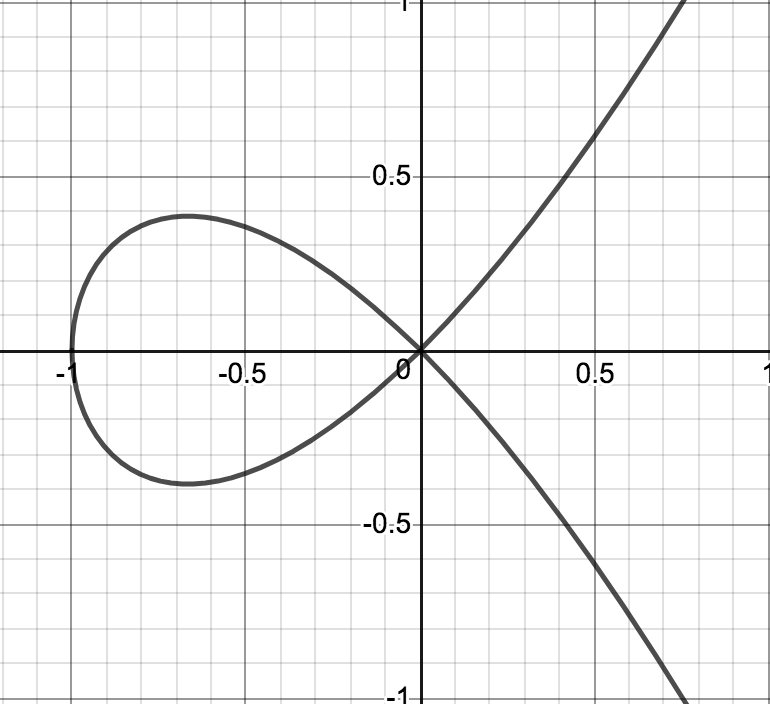
\includegraphics[width=0.3\textwidth]{30.png}
    \caption{The Tschirnhausen cubic. Plotted in Desmos.}
\end{figure}

Recall Hilbert's Nullstellensatz: let $k$ be algebraically closed and $R:=k[X_1,\dotsc,X_{n+1}]$. 
\begin{enumerate}
    \item If $J\subsetneq R$ is a proper ideal, then $V_a(J)\neq\emptyset$.
    \item Every maximal ideal $\mathfrak{m}\subsetneq R$ is of the form $\vbrack{X_1-a_1,\dotsc,X_n-a_n}$ for some point $P=(a_1,\dotsc,a_n)\in\mathbb{A}^2$.
    \item $I_a(V_a(J))=\sqrt{J}$.
\end{enumerate}
Note the distinction for $I_a$ and $V_a$. The subscript ``$a$'' means affine, to distinguish from the projective analogue.

The affine Nullstellensatz carries over, with some caveats. The first condition wobbles, because of the \ita{irrelevant ideal}:
\begin{equation}
    \mathfrak{m_{:(}}:=\vbrack{X_1,\dotsc,X_{n+1}}\subset k[X_1,\dotsc,X_{n+1}]
\end{equation}
Note that $\mathfrak{m}_{:(}$ is indeed a maximal ideal (and hence proper), since $1\notin\mathfrak{m}_{:(}$. However $V_p(\mathfrak{m}_{:(})=\emptyset$, because the only common zero would be $[0:\cdots:0]\notin\mathbb{P}^n$. So we modify. 
\begin{theorem}[Projective Nullstellensats]
    Let $k$ be an algebraically closed, and let $R:=k[X_1,\dotsc,X_{n+1}]$. Let $J\subseteq R$ be a homogeneous ideal.
    \begin{enumerate}
        \item $V_p(J)=\emptyset$ if and only if $\mathfrak{m}_{:(}\subseteq\sqrt{J}$.
        \item No analogue: we can't say anything conclusive about maximal ideals :(
        \item If $V_p(J)\neq\emptyset$, then $I_p(V_p(J))=\sqrt{J}$.
    \end{enumerate}
\end{theorem}
\begin{proof}
    We will use the affine Nullstellensatz by relating $\mathbb{P}^n$ to $\mathbb{A}^{n+1}$. We will need a temporary but fun definition:
    \begin{definition}
        Let $S\subseteq\mathbb{P}^n$ be any subset. We define its \ita{cone} in $\mathbb{A}^{n+1}$ as 
        \begin{equation}
            \mathrm{cone}(S):=\{(a_1,\dotsc,a_{n+1}\in\mathbb{A}^{n+1}\mid [a_1:\cdots:a_{n+1}]\in S\}\cup\{\mathbf{0}\},
        \end{equation}
        where $\mathbf{0}\in\mathbb{A}^{n+1}$ is the zero vector.
    \end{definition}
    \underline{Example}: $S:=V_p(X^2+Y^2-Z^2)$ is a circle in $\mathbb{P}^2$. Then $\mathrm{cone}(S)$ is an actual cone in $\real^3$.
    \begin{figure}[H]
        \centering 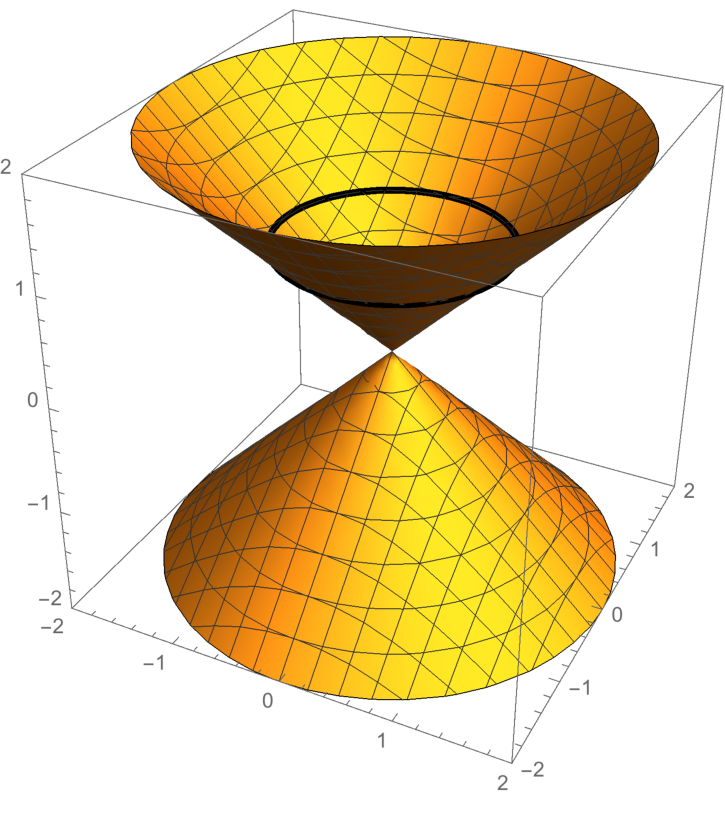
\includegraphics[width=0.3\textwidth]{29.pdf}
        \caption{$\mathrm{cone}(S)$ in $\real^3$. Plotted in \ita{Mathematica}.}
    \end{figure}
    This motivates the term being called ``cone'' in the first place!
    
    Note that if $J\subseteq R$ (remember $R:=k[X_1,\dotsc,X_{n+1}]$) is a proper homogeneous ideal, then $V_a(J)=\mathrm{cone}(V_p(J))$.
    \begin{itemize}
        \item If $J=R$, then $m_P(V)=\emptyset$ (check this) and $\mathfrak{m}_{:(}\subseteq J\subseteq\sqrt{J}$. Otherwise, $J$ is proper, and $V_a(J)=\mathrm{cone}(V_p(J))$. If $V_p(J)=\emptyset$, then $V_a(J)=\{\mathbf{0}\}$, so by affine Nullstellensatz $\sqrt{J}=\vbrack{X_1-0,\dotsc,X_{n+1}-0}=\mathfrak{m}_{:(}$. Conversely, if $\mathfrak{m}_{:(}\subseteq\sqrt{J}$, then for all $i=1\dotsc,n+1$, we have $X_i^{N_i}\subseteq J$ for some $N_i$, so the only common zero of $J$ would be $[0:\cdots:0]$, which is \ita{not} in $\mathbb{P}^n$. So $V_p(J)=\emptyset$. \checkmark
        \item As discussed before, we have $\sqrt{J}\subseteq I_p(V_p(J))$, so we need to prove that $I_p(V_p(J))\subseteq\sqrt{J}$. Let $F\in R$ be a homogeneous polynomial with $F\in I_p(V_p(J))$. So $F$ vanishes on $V_p(J)$. Note that $F$ cannot have a constant term, else it would be a constant (non-zero) polynomial, which does not vanish on $V_p(J)$ (in fact it doesn't vanish anywhere!). Hence $F(\mathbf{0})=0$. So $F$ vanishes on $\mathrm{cone}(V_p(J))=V_a(J)$, so $F\in I_a(V_a(J))$. By affine Nullstellensatz, $F\in\sqrt{J}$, and we are done. \checkmark
    \end{itemize}
\end{proof}
\begin{definition}
    A projective algebraic set $V\subseteq\mathbb{P}^n$ is \ita{irreducible} if it is not the union of two smaller algebraic sets. We call it a \ita{projective variety}.
\end{definition}
\begin{theorem}
    $V\subseteq\mathbb{P}^n$ is a variety if and only if $I_p(V)\subseteq k[X_1,\dotsc,X_{n+1}]$ is prime.
\end{theorem}
The proof of this goes exactly like its affine counterpart.

We again have a correspondence!
\begin{equation}
    \begin{split}
        \{\text{homogeneous radical ideals* in }k[X_1,\dotsc,X_{n+1}]\}&\longleftrightarrow\{\text{projective algebraic sets in }\mathbb{P}^n\}\\
        J&\mapsto V_p(J)\\
        I_p(V)&\mapsfrom V\\
        \text{homogeneous prime ideals}&\longleftrightarrow\text{projective varieties}
    \end{split}
\end{equation}
*except for $\mathfrak{m}_{:(}$ of course!
\section{10 April}
\subsection{Miniquiz}
Graph the zero set of $Z^2-X^2+Y^2$ in $\mathbb{RP}^2$, including any infinite points.
\subsection{Homogenization and Dehomogenization}
\begin{definition}
    Given a polynomial $F\in k[X_1,\dotsc,X_n]$ of degree $s$, we can \ita{homogenize} it into a form $F^*\in k[X_1,\dotsc,X_{n+1}]$. We have two equivalent methods:
    \begin{enumerate}
        \item Decompose $F=F_0+F_1+\dotsb+F_s$ into forms, $F_s\neq0$. Then define 
        \begin{equation}
            F^*:=X_{n+1}^sF_0+X_{n+1}^{s-1}F_1+\dotsb+X_{n+1}^0F_s=\sum\limits_{d=0}^sX_{n+1}^{s-d}F_d.
        \end{equation}
        \item Define 
        \begin{equation}
            F^*:=X_{n+1}^sF\left(\frac{X_1}{X_{n+1}},\dotsc,\frac{X_n}{X_{n+1}}\right).
        \end{equation}
    \end{enumerate}
\end{definition}
\underline{Example}: Let $F$ be the elliptic curve $Y^2-X^3-bX-c$. Then $F^*=ZY^2-bZ^2X-cZ^3$.

Using the second definition, it's easy to see that $(FG)^*=F^*G^*$. But addition fails because terms can cancel. For example, let $F:=X^3+Y^2$, $G:=Y-X^3$. Then $F^*=X^3+ZY^2$, $G^*:=Z^2Y-X^3$, and $F+G=Y^2+Y$. Note that $(F+G)^*=YZ+Y^2$, but $F^*+G^*=Y^2Z+YZ^2$.

The actual identity is
\begin{equation}
    X_{n+1}^t(F+G)^*=X_{n+1}^{\deg(G)}F^*+X_{n+1}^{\deg(F)}G^*,
\end{equation}
where $t:=\deg(F)+\deg(G)-\deg(F+G)$. To check, note that each term is boosted up to degree $=\deg(F)+\deg(G)$.
\begin{definition}
    Given a form $F\in k[X_1,\dotsc,X_{n+1}]$, we can \ita{dehomogenize} it to
    \begin{equation}
        F_*:=F(X_1,\dotsc,X_n,1)\in k[X_1,\dotsc,X_{n+1}].
    \end{equation}
\end{definition}
Note that we can also choose to dehomogenize with respect to another $X_i$ instead of just $X_{n+1}$. We will in fact do this later.

$F\mapsto F_*$ is a ring homomorphism from $k[X_1,\dotsc,X_{n+1}]\to k[X_1,\dotsc,X_n]$ (in fact, it is a $k$-algebra homomorphism!), so $(F+G)_*=F_*+G_*$ and $(FG)_*=F_*G_*$.

Note that $(F^*)_*=F$, but the other composition doesn't work perfectly (left and right inverses yuck!), so we lose powers of $X_{n+1}$ that divide $F$. Instead, we have that $X_{n+1}^t(F_*)^*=F$, where $t$ is maximal such that $X_{n+1}^t\mid F$.
\begin{lemma}[Rehomogenization Lemma]
    Let $F,G\in k[X,Y,Z]$ be forms such that $F_*=G_*$. Then there exists an integer $r\in\z$ such that $F=Z^rG$.
\end{lemma}
\begin{proof}
    Homework.
\end{proof}
\subsection{Geometric Correspondence between $\mathbb{P}^n$ and $\mathbb{A}^n$}
For each $i=1,\dotsc,n+1$, define
\begin{equation}
    \begin{split}
        U_i&=\{[a_1:\cdots:1_i:\cdots:a_{n+1}]\}\subset\mathbb{P}^n\\
        &=\{P\in\mathbb{P}^n\mid\pi_i(P)=1\}.
    \end{split}
\end{equation}
$U_i$ is the set of all points in $\mathbb{P}^n$ with a 1 in the $i$th coordinate. 

Note that $\mathbb{P}^n=\bigcup\limits_{i=1}^{n+1}U_i$, since every $P\in\mathbb{P}^n$. And we have a bijection
\begin{equation}
    \begin{split}
        \phi_i&:\mathbb{A}^n\stackrel{\sim}{\longrightarrow}U_i\\
        &:(a_1,\dotsc,a_n)\mapsto[a_1:\cdots:a_{i-1}:1:a_i:\cdots:a_n]
    \end{split}
\end{equation}
$\stackrel{\sim}{\longrightarrow}$ means bijection.

For example, with $n=2$, we have $\phi_3:\mathbb{A}^3\stackrel{\sim}{\longrightarrow}U_3\subseteq\mathbb{P}^2$ defined by $\phi_3:(a_1,a_2)\mapsto[a_1:a_2:1]$.
\begin{remark}
   The notation and the general idea is very suggestive. Can we say that the $\phi_i$'s are charts, the $U_i$'s are open neighborhoods, and that the collection $\{(U_i,\phi_i,)\}_{i=1}^n$ is our atlas? In the case of $\mathbb{RP}^n$, definitely! However, we have to be careful since we usually want $k$ to be algebraic, and so our $\mathbb{P}^n(k)$ may not have a (real) manifold structure anymore. Take this geometric correspondence as you will.
\end{remark}
\subsection{Coordinate Rings [Handout]}
As with affine algebraic sets, we can define the coordinate ring of a projective algebraic set and the local ring at a point:
\begin{definition}
    Let $V\subseteq\mathbb{P}^n$ be a projective variety, so $I(V)$ is a prime ideal. The \ita{homogeneous coordinate ring} of $V$ is 
    \begin{equation}
        \Gamma_H(V):=k[X_1,\dotsc,X_{n+1}]/I(V).
    \end{equation}
    The subscript ``$H$'' is for ``homogeneous.'' It  is a domain.
\end{definition}
Why only varieties and not all algebraic sets? Because we want to define functions, and we'll see below that in order to do that, we'll need the field of fractions of $\Gamma_H(V)$. So we need $\Gamma_H(V)$ to be a domain. We can speak of forms in $\Gamma_H(V)$. In fact, let $J\subseteq k[X_1,\dotsc,X_{n+1}]$ be any homogeneous ideal and let $\Gamma:=k[X_1,\dotsc,X_{n+1}]/J$.
\begin{definition}
    $f\in\Gamma$ is a \ita{form of degree d} if there is a form $F\in k[X_1,\dotsc,X_{n+1}]$ of degree $d$ such that $\overline{F}=f$.
\end{definition}
Is this well-defined? Suppose $f=\overline{F}=\overline{G}$, where $F,G\in k[X_1,\dotsc,X_{n+1}]$ are forms of degree $d\neq e$, respectively. Then $F\equiv G$ (mod $J$), so $F-G\in J$, so by homogeneity of $J$, we get $F\in J$ and $G\in J$. So $f=\overline{0}$.
\begin{lemma}[Decomposition Fact]
    Every $f\in\Gamma$ can be written uniquely as $f=f_0+f_1+\dotsb+f_m$, where $f_d$ is a form of degree $d$.
\end{lemma}
\begin{proof}
    \begin{itemize}
        \item Existence: Write $f=\overline{F}$ for some $F\in k[X_1,\dotsc,X_{n+1}]$ and decompose $F=F_0+\dotsb+F_m$ into forms. Then $f=\overline{F_0}+\dotsb+\overline{F_m}=:f_0+f_1+\dotsb+f_m$.
        \item Uniqueness: Suppose $f=\overline{F_0}+\dotsb+\overline{F_m}=\overline{G_0}+\dotsb+\overline{G_m}$ for forms $F_d,G_d\in k[X_1,\dotsc,X_{n+1}]$. Then $(F_0-G_0)+\dotsb+(F_m-G_m)\in J$, so by homogeneity of $J$, we have that all $(F_d-G_d)\in J$, so $\overline{F_d}=\overline{G_d}$.
    \end{itemize}
\end{proof}
\subsection{Rational Functions [Handout]}
Since $\Gamma_H(V)$ is a domain, we can take its field of fractions, which we call $\underline{k_H(V)}$, the \ita{homogeneous function field} of $V$.

Our problem is that functions on points $P\in V$ might not be well defined. Even if $F\in k[X_1,\dotsc,X_{n+1}]$ is a form of degree $d$, we have
\[F(\lambda a_1,\dotsc,\lambda a_{n+1})=\lambda^d F(a_1,\dotsc,a_{n+1}).\]
To fix this, we look at quotients of forms equal degree. Note that if $f,g\in\Gamma_H(V)$ are forms of degree $d$, then $f=\overline{F}$, $g=\overline{G}$, where $F,G\in k[X_1,\dotsc,X_{n+1}]$ are forms of degree $d$. For $P=[a_1:\cdots:a_{n+1}]\in\mathbb{P}^n$, we can define
\[\frac{f}{g}(P):=\frac{F(a_1,\dotsc,a_{n+1}}{G(a_1,\dotsc,a_{n+1})}\]
so long as $G(a_1,\dotsc,a_{n+1})\neq0$. Note that this is independent of the lifts $F$ and $G$ of $f$ and $g$, and it's also independent of the representation $P=[a_1:\cdots:a_{n+1}]$.
\begin{definition}
    The \ita{function field} of $V$ is
    \begin{equation}
        k(V):=\left\{\frac{f}{g}\in k_H(V)\middle|\,f,g\in\Gamma_H(V)\text{ are forms of \ita{equal} degree }\right\}.
    \end{equation}
\end{definition}
\begin{remark}
   A warning on notation: $k(V)\subsetneq k_H(V)$!
\end{remark}
Note that $k(V)$ is a field, since if $\deg f_1=\deg g_1=d$ and $\deg f_2=\deg g_2=e$, then $\frac{f_1}{g_1}\cdot\frac{f_2}{g_2}=\frac{f_1f_2}{g_1g_2}$ and $\frac{f_1}{g_1}+\frac{f_2}{g_2}=\frac{f_1g_2+f_2g_1}{g_1g_2}$ and
\[\deg(f_1f_2)=\deg(g_1g_2)=\deg(f_1g_2+f_2g_1)=d+e.\]
\begin{definition}
    Let $P\in V$ and $z=\frac{f}{g}\in k(V)$. We define $z(P):=\frac{f(P)}{g(P)}$ if $g(P)\neq0$.
\end{definition}
\begin{definition}
    The \ita{local ring} of $V$ at $P$ is
    \begin{equation}
        \mathcal{O}_P(V):=\{z\in k(V)\mid z\text{ is defined at }P\}=\left\{\frac{f}{g}\in k(V)\middle|\,g(P)\neq0\right\}.
    \end{equation}
    This is local with maximal ideal
    \begin{equation}
        \mathfrak{m}_P(V):=\{z\in\mathcal{O}_P(V)\mid z(P)=0\}=\left\{\frac{f}{g}\in\mathcal{O}_P(V)\middle|\,f(P)=0\right\}.
    \end{equation}
\end{definition}
\subsection{Algebraic Correspondence}
Note that for $V:=\mathbb{P}^n$, we have the following:
\begin{itemize}
    \item $I(\mathbb{P}^2)=\{0\}$.
    \item $\Gamma_H(\mathbb{P}^2):=k[X,Y,Z]/I(\mathbb{P}^2)=k[X,Y,Z]$.
    \item $k_H(\mathbb{P}^2):=$ field of fractions of $k[X,Y,Z]=k(X,Y,Z)$.
    \item $k(\mathbb{P}^2)=\left\{\frac{F}{G}\middle|\,F,G\in k[X,Y,Z],G\neq0,F\text{ and }G\text{ are both forms of equal degree }\right\}$.
\end{itemize}
Back in $\mathbb{A}^2$, we have a similar set-up:
\[k(\mathbb{A}^2)=\left\{\frac{F}{G}\middle|\,F,G\in k[X,Y],G\neq0\right\}.\]
This gives us a correspondence of function fields:
\begin{align*}
    \alpha:k(\mathbb{P}^2)&\to k(\mathbb{A}^2)\\
    \frac{F}{G}&\mapsto\frac{F_*}{G_*}
\end{align*}
$\alpha$ is actually an isomorphism (check this for yourself).\\\\
\underline{Example}: In $\mathbb{P}^2$, look at $P:=[a_1:a_2:1]\in U_3=\phi_3(\mathbb{A}^2)\subset\mathbb{P}^2$. $P$ has an inverse image $\phi_3^{-1}(P)=(a_1,a_2)\in\mathbb{A}^2$. We claim that $\alpha$ restricts to an isomorphism of local rings:
\[\alpha:\mathcal{O}_P(\mathbb{P}^2)\stackrel{\sim}{\longrightarrow}\mathcal{O}_{\phi_3^{-1}(P)}(\mathbb{A}^2).\]
This is because for a denominator $G(X,Y,Z)$, we have that
\begin{align*}
    G(P)&=G(a_1,a_2,1)\\
    &=G_*(a_1,a_2)\\
    &=G_*(\phi_3^{-1}(P)).
\end{align*}
So our denominator is non-zero if and only if the other one is also non-zero.\\\\
Why do we care? We will define intersection numbers in $\mathbb{P}^n$ by dehomogenizing to a $U_i$ and applying old machinery from $\mathbb{A}^n$. Is this well-defined? If $P$ belongs to multiple $U_i$'s, then the local rings in the different $U_i$'s will all be isomorphic to a gold standard local ring in $\mathbb{P}^2$. So this is well-defined. \checkmark
\section{15 April}
\subsection{Miniquiz}
Let $F:=X^4+2X^3+Y^2+3XY+7$. Homogenize $F$ in $k[X,Y,Z]$, then dehomogenize at $Y$ (not at $Z$!) to get an answer in $k[X,Z]$.
\subsection{Projective Plane Curves}
Recall from last time:
\begin{itemize}
    \item Homogenization at $Z$: $F(X,Y)\in k[X,Y]\mapsto F^*(X,Y,Z)\in k[X,Y,Z]$
    \item Dehomogenization at $Z$: $F(X,Y,Z)\in k[X,Y,Z]\mapsto F_*(X,Y)\in k[X,Y]$
\end{itemize}
We have an atlas $\{(U_i,\phi_i)\}_{i=1}^n$ for $\mathbb{P}^n$. For $\mathbb{P}^2$, we had the specific charts:
\begin{itemize}
    \item $\phi_1:\mathbb{A}^2\stackrel{\sim}{\longrightarrow}U_1:=\{[1:a_2:a_3]\in\mathbb{P}^2\mid a_2,a_3\in k\}\subsetneq\mathbb{P}^2$, $(a_2,a_3)\mapsto[1:a_2:a_3]$
    \item $\phi_2:\mathbb{A}^2\stackrel{\sim}{\longrightarrow}U_2:=\{[a_1:1:a_3]\in\mathbb{P}^2\mid a_1,a_3\in k\}\subsetneq\mathbb{P}^2$, $(a_1,a_3)\mapsto[a_1:1:a_3]$
    \item $\phi_3:\mathbb{A}^2\stackrel{\sim}{\longrightarrow}U_3:=\{[a_1:a_2:1]\in\mathbb{P}^2\mid a_1,a_2\in k\}\subsetneq\mathbb{P}^2$, $(a_1,a_2)\mapsto[a_1:a_2:1]$
\end{itemize}
\begin{definition}
    For $F\in k[X,Y]$, we call $V(F^*)\subset\mathbb{P}^2$ the \ita{projective closure} of $V(F)\subset\mathbb{A}^2$.
\end{definition}
\begin{remark}
   If we put the manifold topology on $\mathbb{P}^2$, this corresponds exactly to the closure of $\bigcup\limits_{i=1}^3\phi_i(V(F))$.
\end{remark}
\underline{Example}: Let $F:=Y^2-X^2-1$. Then $V(F^*)=V(Y^2-X^2-Z^2)$. 
\begin{figure}[H]
    \centering
    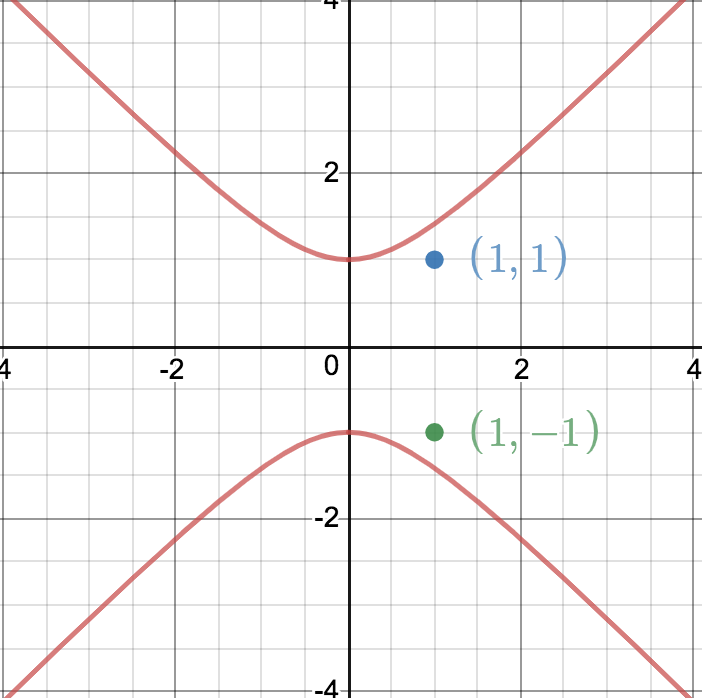
\includegraphics[width=0.3\textwidth]{31.png}
    \caption{$V(F^*)$ as plotted in $\mathbb{A}^2(\real)$. The points $(1,1)$ and $(1,-1)$ correspond to the infinite points $[1:1:0]$ and $[1:-1:0]$. Plotted in Desmos.}
\end{figure}
This hyperbola and the two infinite points is actually a closed loop!

Note that $\phi_3(V(F))=V(F^*)\cap U_3$. In the other direction, for a form $F\in k[X,Y,Z]$, we have $V_p(F)\cap U_3=\phi_3(V_a(F_*))$.\\\\
\underline{Wee Problem}: Irreducibility is not preserved!\\\\
\underline{Example}: Let $F:=YZ^2-X^2Z=(YZ-X^2)Z$ is not irreducible, but $F_*=Y-X^2$ is irreducible.

We have a clumsy solution to this wee problem: 
\begin{claim}
    Let $F\in k[X,Y,Z]$ be a form such that $Z\nmid F$ (in general $X_{n+1}\nmid F$). Then $F$ is irreducible if and only if $F_*$ is.
\end{claim}
\begin{proof}
    Homework.
\end{proof}
\begin{definition}
    Two forms $F,G\in k[X,Y,Z]$ are \ita{equivalent} if $F=\lambda G$ for some $\lambda\in k^{\times}$. A \ita{projective plane curve} is an equivalence class of forms.
\end{definition}
Let $F$ be a projective plane curve. Then
\begin{equation}
    V(F)=\bigcup\limits_{i=1}^3V(F)\cap U_i=\bigcup\limits_{i=1}^3\phi_i(V_a(F_*)),
\end{equation}
where the dehomogenization is taken with respect to the $i$th variable.
\begin{definition}
    Let $F$ be a projective plane curve, and let $P\in U_i\cap F$. Then we define
    \begin{equation}
        m_P(F):=m_{\phi_i^{-1}(P)}(F_*).
    \end{equation}
\end{definition}
\underline{Example}: Let $F:=Y^2Z-X^3-X^2Z$. Then $F_*$ is our familiar Tschirnhausen cubic.
\begin{figure}[H]
    \centering
    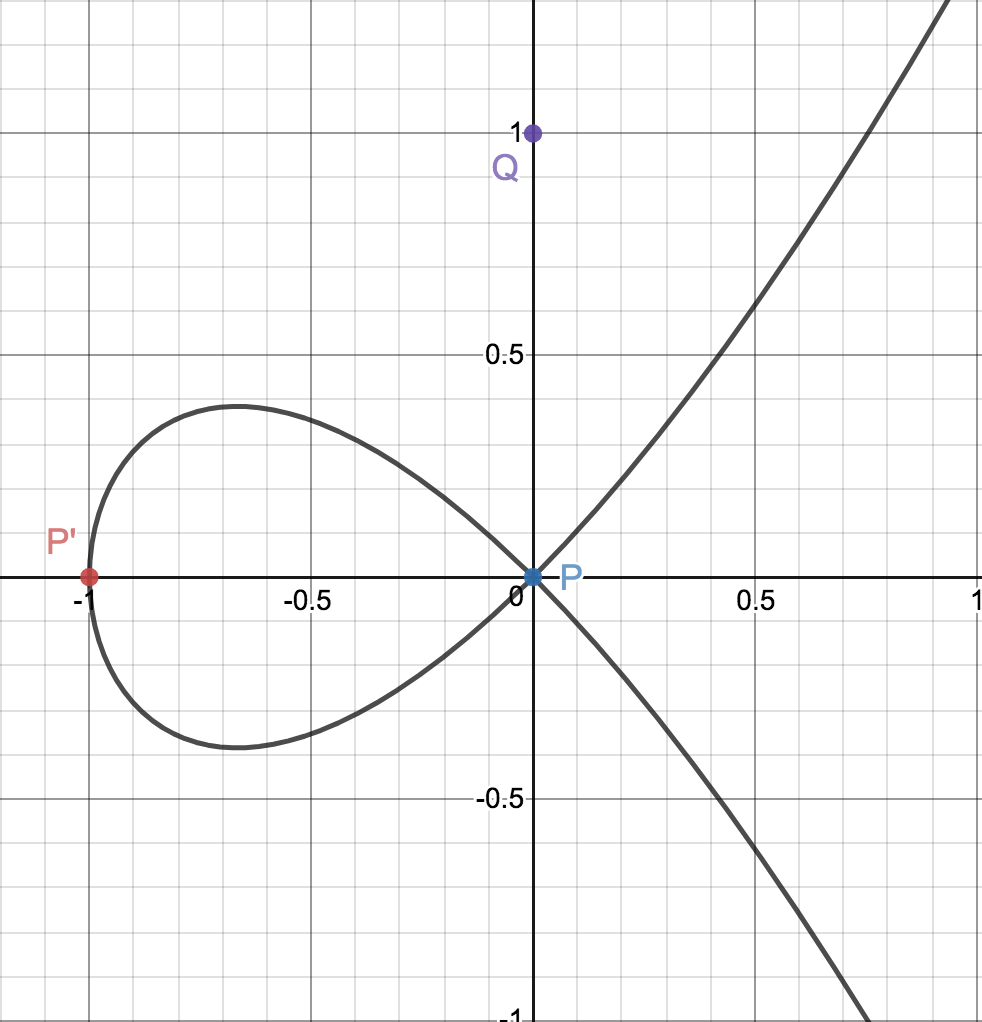
\includegraphics[width=0.3\textwidth]{32.png}
    \caption{$V(F_*)$ as plotted in $\mathbb{A}^2(\real)$. The point $(0,1)$ corresponds to the infinite points $[0:1:0]$. Plotted in Desmos.}
\end{figure}
\begin{itemize}
    \item Let $P:=[0:0:1]=\phi_3((0,0))$. Then
    \begin{align*}
        m_P(F)&=m_{\phi_3^{-1}(P)}(F_*)\\
        &=m_{(0,0)}(Y^2-X^3-X^2)\\
        &=\boxed{2.}
    \end{align*}
    \item Let $P':=[-1:0:1]$. Then $m_{P'}(F)=1$ as expected!
    \item We also have the infinite point $Q:=[0:1:0]$. This time we have to use $\phi_2$:
    \begin{align*}
        m_Q(F)&=m_{\phi_2^{-1}(Q)}(F_*)\\
        &=m_{(0,0)}(Z-X^3-X^2Z)\\
        &=1.
    \end{align*}
\end{itemize}
\begin{figure}[H]
    \centering
    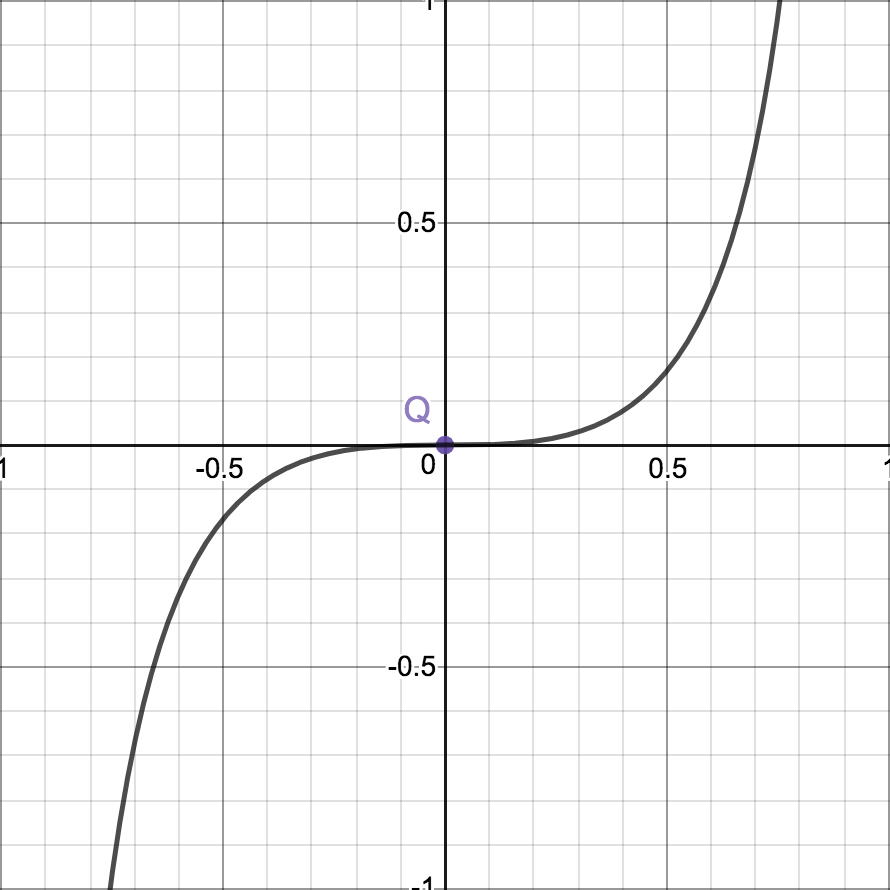
\includegraphics[width=0.3\textwidth]{33.png}
    \caption{$V_p(F)\cap U_2$ as plotted in $\mathbb{A}^2(\real)$. The point $(0,0)$ corresponds to the infinite points $[0:1:0]$. Plotted in Desmos.}
\end{figure}
We have a few concerns:
\begin{enumerate}
    \item Is $m_P(F)$ well-defined? In our examples, the points were in only one of the $U_i$'s, but in general $P$ may lie in multiple $U_i$'s. Does $m_P(F)$ depend on $U_i$?
    
    As it turns out, we have a soothing answer: not at all!
    \begin{proof}
        Recall the Dimension and Multiplicity Theorem: For all $n$ sufficiently large, we have
        \[m_P(F_*)=\dim_k\left[\mathfrak{m}_P^n(F_*)/\mathfrak{m}_P^{n+1}(F_*)\right].\]
        So $m_{\phi_i^{-1}(P)}(F_*)$ depends only on the structure of the local ring at $\phi_i^{-1}(P)$. But (from last time) we found an isomorphism $\alpha:\mathcal{O}_P(V)\to\mathcal{O}_{\phi_i^{-1}(P)}$. So whichever $i$ we pick, we will get the same answer.
    \end{proof}
    \item Technically, the Dimension and Multiplicity Theorem requires $F$ to be \ita{irreducible}. We have a less soothing solution for this one: homework.
\end{enumerate}
\subsection{Intersection Numbers in $\mathbb{P}^n$}
Let $F,G$ be projective plane curves and let $P\in\mathbb{P}^2$.
\begin{definition}
    The intersection number of $F$ and $G$ at $P$ is
    \begin{equation}
        \boxed{I_P(F,G):=I_{\phi_i^{-1}(P)}(F_*,G_*).}
    \end{equation}
    This is of course equal to $\dim_k\left[\mathcal{O}_{\phi_i^{-1}(P)}(\mathbb{A}^2)/\vbrack{F_*,G_*}\right]$.
\end{definition}
\underline{Example}: Let $F:=YZ-X^2$, $G:=Y^2Z-X^3-X^2Z$. They both have the infinite point $P:=[0:1:0]$. Find $I_P(F,G)$:
\begin{align*}
    I_P(F,G)&=I_{\phi_2^{-1}(P)}(F_*,G_*)\\
    &=I_{(0,0)}(Z-X^2,Z-X^3-X^2Z)\\
    &=I_{(0,0)}(Z-X^2,X^2-X^3-X^4)\\
    &=I_{(0,0)}[(Z-X^2,X^2(1-X-X^2))]\\
    &=I_{(0,0)}(Z-X^2,X^2)+I_{(0,0)}(Z-X^2,1-X-X^2)\\
    &=I_{(0,0)}(Z,X^2)\\
    &=2I_{(0,0)}(Z,X)\\
    &=\boxed{2.}
\end{align*}
$m_P(F_*)=m_P(G_*)=1$, but they share a tangent line $Z=0$, an infinite tangent line! We can kinda see why $I_P(F,G)=2$ if we look at their plots in the $X$-$Z$ plane:
\begin{figure}[H]
    \centering
    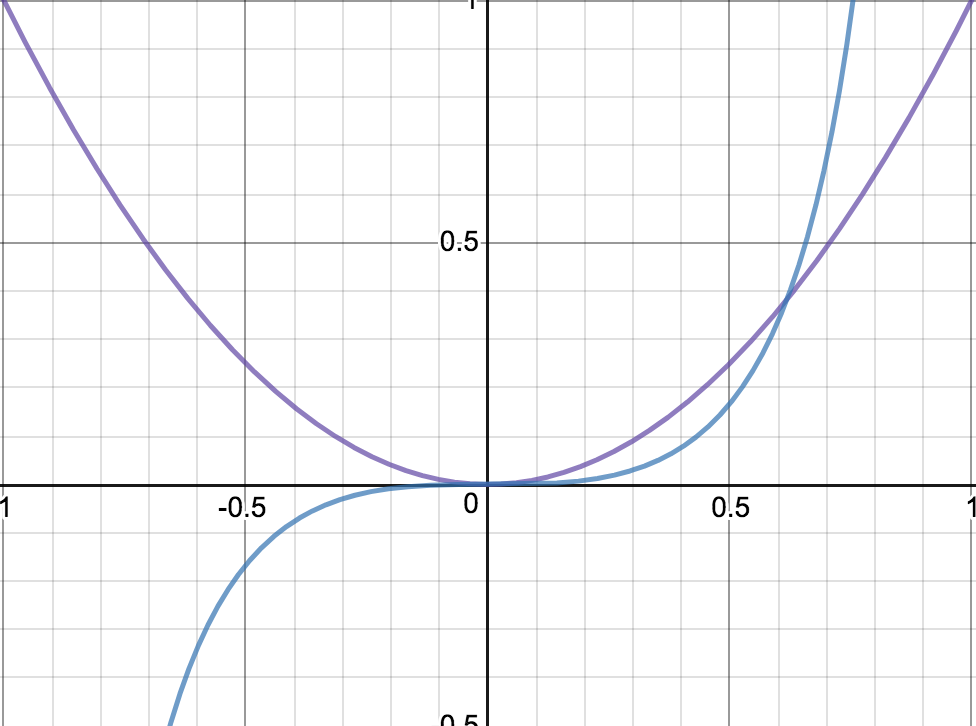
\includegraphics[width=0.3\textwidth]{34.png}
    \caption{$V_p(F)\cap U_2$ and $V_p(G)\cap U_2$ as plotted in $\mathbb{A}^2(\real)$. Plotted in Desmos.}
\end{figure}
\subsection{The Yellow Brick Road to B\'ezout}
It turns out calling it ``the Yellow Brick Road'' might not have had the intended effect. Or does it $\dotsc$
\begin{theorem}[Projective Finite Intersection Theorem]
    Let $F,G$ be projective plane curves that share no common component. Then $V_p(F,G)=V_p(F)\cap V_p(G)$ is finite.
\end{theorem}
\begin{proof}
    Since $\mathbb{P}^2=\bigcup\limits_{i=1}^3U_i$, we have $V_p(F,G)=\bigcup\limits_{i=1}^3V_p(F,G)\cap U_i$, so it suffices to show that each $V_p(F,G)\cap U_i$ is finite. Consider $i=3$. Any $P\in U_3$ is of the form $[a_1:a_2:1]$, so if $P\in V_p(F,G)$, then $\phi_3^{-1}(P)=(a_1,a_2)\in V_a(F_*,G_*)$. By the Affine Finite Intersection Theorem, $V_a(F_*,G_*)$ is finite and so we are done.
\end{proof}
\section{17 April}
\subsection{Miniquiz}
The projective closures of the hyperbolae $F:=XY-1$ and $G:=XY+1$ both contain the infinite point $[1:0:0]$. Find their intersection number there.
\subsection{Road to B\'ezout's Theorem}
From last time, we defined intersection numbers in projective space by pulling back to affine space:
\[I_P(F,G):=I_{\phi_i^{-1}(P)}(F_*,G_*),\]
where $P\in U_i$ and we can dehomogenize at \ita{any} coordinate where $P$ is non-zero.

Assume $k$ is algebraically closed.
\begin{lemma}[Dodger Lemma]
    Given any finite set $S\subset\mathbb{P}^2$, there is a line that avoids all of $S$.
\end{lemma}
\begin{proof}
    Homework.
\end{proof}
\begin{lemma}[Cancellation Lemma]
    Let $F$ and $G$ be projective plane curves with no common component. Assume that $V(F,G,Z)=\emptyset$, \ita{i.e.}, $F$ and $G$ don't intersect at $L_{\infty}:=V(Z)$. Then for $HZ\in\vbrack{F,G}\subseteq k[X,Y,Z]$, $H\in\vbrack{F,G}$. So we can cancel $Z$!
\end{lemma}
\begin{proof}
    Write $HZ=AF+BG$ for some $A,B\in k[X,Y,Z]$, and organize everything by powers of $Z$: Write $A=A_0+A_1Z$, $B=B_0+B_1Z$, $C=C_0+C_1Z$, with $A_0,B_0,C_0\in k[X,Y]$. We claim that $F_0$ and $G_0$ are relatively prime in $k[X,Y]$. If not, suppose that a non-unit $D(X,Y)$ divides $F_0$ and $G_0$. Using algebraic closure, find a $(x_0,y_0)\neq(0,0)$ such that $D(X_0,y_0)\neq0$. Then $[x_0:y_0:0]\in V(F,G,Z)$, a contradiction. This proves the claim.
    
    Taking $Z:=0$ in $HZ=AF+BG$ gives $0=A_0F_0+B_0G_0\Rightarrow-A_0F_0=B_0G_0$ in $k[X,Y]$, which is a UFD. So $F_0\mid B_0G_0$, and since $F_0$ and $G_0$ are relatively prime then $F_0\mid B_0\Rightarrow B_0=CF_0$ for some $C\in k[X,Y]$. So $-A_0F_0=CF_0G_0\Rightarrow-A_0=CG_0$. Plug everything back into:
    \begin{align*}
        HZ&=AF+BG\\
        &=(A_0+A_1Z)F+(B_0+B_1Z)G\\
        &=(-CG_0+A_1Z)F+(CF_0+B_1Z)G\\
        &=[-C(G-G_1Z)+A_1Z]F+[C(F-F_1Z)+B_1Z]G\\
        &=(CG_1Z+A_1Z)F+(-CF_1Z+B_1Z)G\\
        \Rightarrow H&=(CG_1+A_1)F+(B_1-CF_1)G\\
        &\in\vbrack{F,G}.\checkmark
    \end{align*}
\end{proof}
\subsection{B\'ezout's Theorem}
\begin{theorem}[B\'ezout's Theorem]
    Let $F$ and $G$ be projective plane curves with no common components. Then
    \begin{equation}
        \boxed{\sum\limits_{P\in\mathbb{P}^2}I_P(F,G)=(\deg F)(\deg G).}
    \end{equation}
\end{theorem}
\begin{remark}
   By the Projective Finite Intersection Theorem, $I_P(F,G)=0$ for all but finitely many $P\in\mathbb{P}^2$, so the sum is well-defined.
\end{remark}
\underline{Example}: Let $F:=Y^2-X^3$, $G:=Y-X^2$, $H:=X-Y^2$.
\begin{figure}[H]
    \centering
    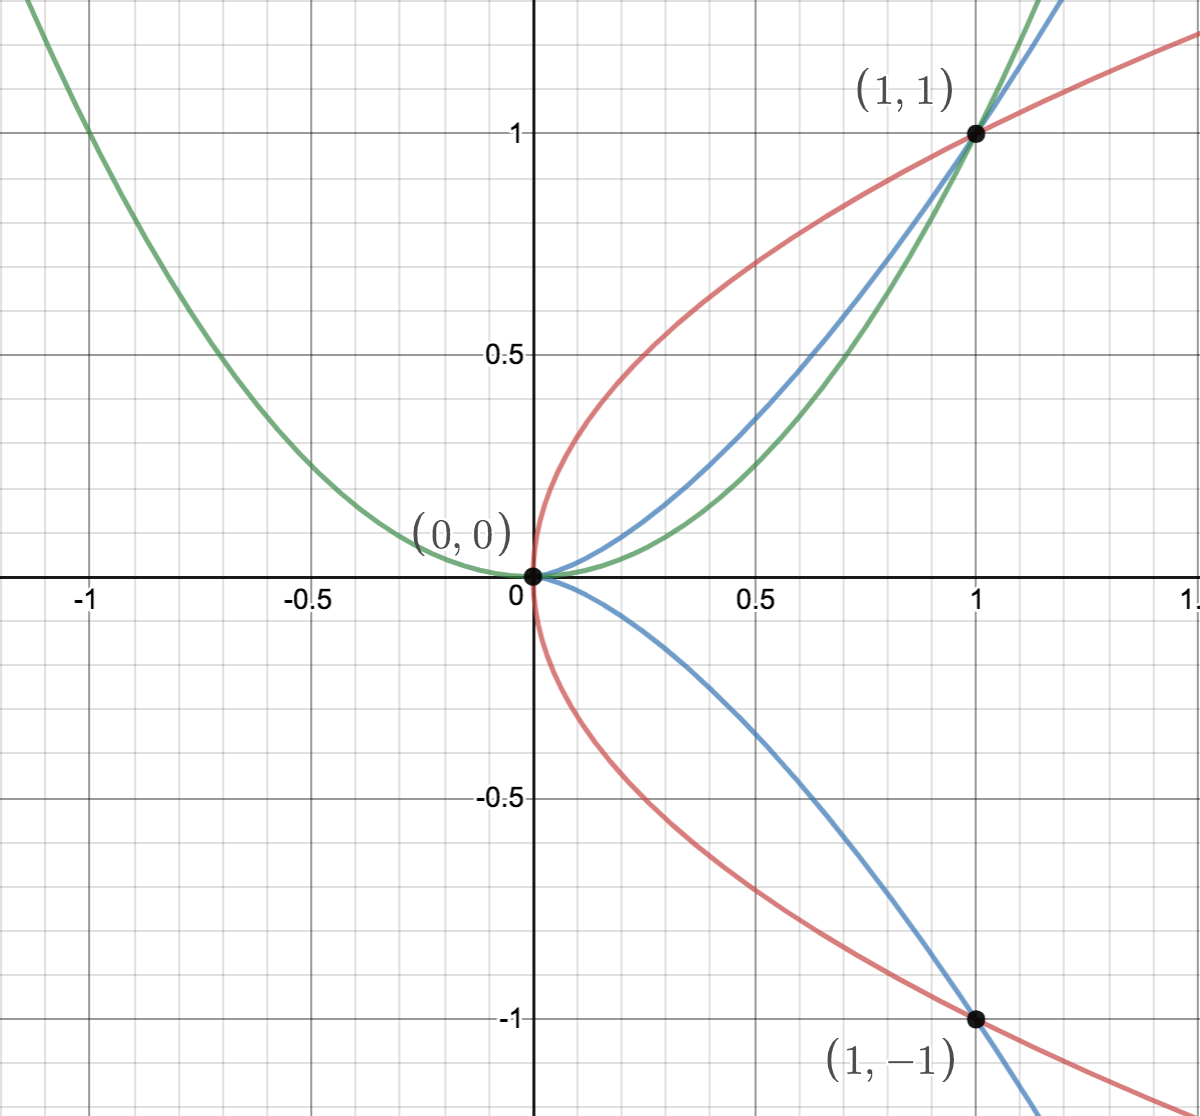
\includegraphics[width=0.3\textwidth]{35.png}
    \caption{$V(F)$, $V(G)$, and $V(H)$ as plotted in $\mathbb{A}^2$. Plotted in Desmos.}
\end{figure}
According to B\'ezout,
\begin{enumerate}
    \item $F$ and $G$ should have $\boxed{6}$ intersections.
    \item $F$ and $H$ should also have $\boxed{6.}$
    \item $G$ and $H$ should have $\boxed{4.}$
\end{enumerate}
Note that we are not able to see all of the intersections in Figure 35, due to several reasons:
\begin{enumerate}
    \item Several of the intersection points on the graph are multiple points.
    \item We have to consider infinite points.
    \item $k$ is algebraically closed!
\end{enumerate}
\begin{proof}
    By the Projective Finite Intersection Theorem, $V(F,G)$ is finite. So by the Dodger Lemma, there is a line in $\mathbb{P}^2$ avoiding all of their intersections. Run a projective change of coordinates (see Homework 11 for definition) to take this line to the infinite line $Z=0$ ($L_{\infty}$). So we may assume that $F$ and $G$ only intersect in $U_3\cong\mathbb{A}^2$ (what equivalence is this by the way?) Then we calculate
    \begin{align*}
        \sum\limits_{P\in\mathbb{P}^2}I_P(F,G)&=\sum\limits_{P\in\mathbb{A}^2}I_P(F_*,G_*)\\
        &=\sum\limits_{P\in\mathbb{A}^2}\dim_k[\mathcal{O}_P(\mathbb{A}^2)/\vbrack{F_*,G_*}]\\
        &=\dim_k(k[X,Y]/\vbrack{F_*,G_*})&&\text{by Dimension Theorem.}
    \end{align*}
    As an aside, here is a guide for the rest of the proof:
    \begin{itemize}
        \item Let $S:=k[X,Y,Z]$, $\Gamma:=S/\vbrack{F,G}$. For $H\in S$, $\overline{H}:=H+\vbrack{F,G}$ (coset).
        \item $S_d\subset S$ are forms of degree $d$, $\Gamma_d:=\pi(S_d)=\{\text{forms of degree }d\text{ in }\Gamma.\}$
        \item Let $\Gamma_*:=k[X,Y]/\vbrack{F_*,G_*}$. For $H\in k[X,Y]$, $\Hat{H}:=H+\vbrack{F_*,G_*}$ (coset).
        \item Recall the \underline{Pyramid Lemma}: $\dim_k(S_d)=\frac{1}{2}(d+1)(d+2)$.
    \end{itemize}
    Now let's resume the proof. Let $m:=\deg F$, $n:=\deg G$.
    \begin{claim}[1]
        For $d\geq m+n$, we have $\dim_k(\Gamma_d)=mn$.
    \end{claim}
    \begin{proof}
        Set up a not-so-short exact sequence of vector spaces:
        \begin{equation}
            \{0\}\xlongrightarrow{} S\xlongrightarrow{\psi}S\times S\xlongrightarrow{\phi}S\xlongrightarrow{\pi}\Gamma\xlongrightarrow{}\{0\},
        \end{equation}
        where
        \begin{itemize}
            \item $\psi:C\mapsto(CG,-CF)$,
            \item $\phi:(A,B)\to AF+BG$, and
            \item $\pi:H\to\overline{H}$.
        \end{itemize}
    Let's check exactness:
    \begin{enumerate}
        \item $\psi$ is injective because $S$ is a domain. \checkmark
        \item $\mathrm{Im}\psi\stackrel{?}{=}\ker\phi$: $\subseteq$ is clear because $\phi(CG,-CF)=CGF-CFG=0$. For $\supseteq$, if $(A,B)\in\ker\phi$, then $AF=-BG$. Since $F$ and $G$ have no common components, $F\mid(-B)$. Say $FC=-B$. Then $AF-FCG=0\Rightarrow A=CG$. Then $(A,B)=(CG,-CF)=\psi(C)$. \checkmark
        \item $\mathrm{Im}\phi\stackrel{?}{=}\ker\pi$: $\mathrm{Im}\phi=\vbrack{F,G}=\overline{0}$. \checkmark
        \item $\pi$ is surjective. \checkmark
        \end{enumerate}
        The analogue of Exact Dimension Theorem for this not-so-short exact sequence gives us that
        \[\dim_k(S_{d-(n+m)})+\dim_k(S_d)=\dim_k(S_{d-m}\times S_{d-n})+\dim_k(\Gamma_d).\]
        Using the Pyramid Lemma, we have
        \begin{align*}
            \frac{1}{2}[d-(m+n)+1][d-(m+n)+2]+\frac{1}{2}(d+1)(d+2)&=\frac{1}{2}(d-m+1)(d-m+1)\\
            &+\frac{1}{2}(d-n+1)(d-n+2)+\dim_k(\Gamma_d)\\
            \Rightarrow\dim_k(\Gamma_d)&=mn.
        \end{align*}
    \end{proof}
    We're not yet done with the proof of B\'ezout!
\end{proof}
\section{22 April}
\subsection{Miniquiz}
Let $F:=Y^2-X^3$, $G:=Y^2-X^3+X$. Besides the origin, how many \ita{other} intersection points in $\mathbb{CP}^2$ should we expect (counted with multiplicity)?
\subsection{Proof of B\'ezout's Theorem (cont'd)}
From last time, we proved Claim 1, which stated that $\dim_k(\Gamma_d)=mn$. Now move on to another claim:
\begin{claim}[2]
    The map $\Gamma\to\Gamma$ defined by $\overline{H}\mapsto\overline{ZH}$ is injective.
\end{claim}
\begin{proof}
    This is the Cancellation Lemma: if $\overline{ZH}=\overline{0}$, then $ZH\in\vbrack{F,G}$, and so we can cancel $Z$ to get $H\in\vbrack{F,G}$. Thus $\overline{H}=\overline{0}$.
\end{proof}
Newt, we show that $\dim_k(\Gamma_*)=mn$. By Claim 1, we know that $\dim_k(\Gamma_{m+n})=mn$, so it has a basis of $mn$ forms. Let $H_1,\dotsc,H_{mn}\in S_{m+n}$ be such that $\{\overline{H_1},\dotsc,\overline{H_{mn}}\}$ is a basis for $\Gamma_{m+n}$. 
\begin{claim}[3]
    $\{\widehat{H_{1*}},\dotsc,\widehat{H_{mn*}}\}$ is a basis for $\Gamma_*$. Proving this will finish B\'ezout.
\end{claim}
\begin{proof}
    To prove that any collection is a basis, we need to show that they span the vector space and are linearly independent:
    \begin{itemize}
        \item Spanning set: Let $f\in k[X,Y]$ and homogenize it to $f^*\in k[X,Y,Z]$. If $\deg f^*<m+n$, then multiply by enough powers of $Z$ such that $Z^tf^*\in S_{m+n}$. If $\deg f^*\geq m+n$, then we get $f^*\in S_d$ for $d=m+n+r$ for some $r\geq0$. Either way, we get $Z^tf^*\in S_d$, so $\overline{Z^tf^*}\in\Gamma_d$. Recall that $\{\overline{H_1},\dotsc,\overline{H_{mn}}\}$ is a basis for $\Gamma_{m+n}$. Look at $\{\overline{Z^tH_1},\dotsc,\overline{Z^tH_{mn}}\}$ in $\Gamma_d$. These are still linearly independent, since
        \[\sum\limits_{i=1}^{mn}c_i\overline{Z^tH_i}=0\implies\overline{Z^t}\sum\limits_{i=1}^{mn}c_i\overline{H_i}=0\implies\sum\limits_{i=1}^{mn}c_i\overline{H_i}=0,\]
        by Cancellation Lemma, and hence $c_i=0$ for all $i=1,\dotsc,mn$ since $\{\overline{H_1},\dotsc,\overline{H_{mn}}\}$ is a basis. Since $\dim_k(\Gamma_d)=mn$, $\{\overline{Z^tH_1},\dotsc,\overline{Z^tH_{mn}}\}$ is a basis for $\Gamma_d$. So $\overline{Z^tf^*}=\sum\limits_{i=1}^{mn}c_i\overline{Z^tH_i}$ for some $c_i\in k$. So in $S=k[X,Y,Z]$, we have $Z^tf^*-\sum\limits_{i=1}^{mn}c_iZ^tH_i=AF+BG$ for some $A,B\in S$. Dehomogenize this to get $f-\sum\limits_{i=1}^{mn}c_iH_{i*}=A_*F_*+B_*G_*$. Then $\hat{f}=\sum\limits_{i=1}^{mn}c_i\widehat{H_{i*}}$. Hence $\{\widehat{H_{1*}},\dotsc,\widehat{H_{mn*}}\}$ spans $\Gamma_*$. \checkmark
        \item Linear independence: Suppose $\sum\limits_{i=1}^{mn}c_i\widehat{H_{i*}}=\hat{0}$ in $\Gamma_*$ for $c_i\in k$. Then
        \begin{align*}
            \sum\limits_{i=1}^{mn}c_iH_{i*}&=AF_*+BG_*&&\text{for }A,B\in k[X,Y]\\
            &=(A^*)_*F_*+(B^*)_*G_*\\
            \left(\sum\limits_{i=1}^{mn}c_iH_i\right)_*&=(A^*F+B^*G)_*.
        \end{align*}
        By the Rehomogenization Lemma, $\sum\limits_{i=1}^{mn}c_iZ^rH_i=Z^s(A^*F+B^*G)$ in $k[X,Y,Z]$ for some $r,s\geq0$. Then
        \begin{align*}
            \sum\limits_{i=1}^{mn}c_i\overline{Z^rH_i}&=\overline{Z^s(A^*F+B^*G)}\\
            &=\overline{0}&&\text{in }\Gamma=k[X,Y,Z]/\vbrack{F,G}.
        \end{align*}
        By Claim 2, $\sum\limits_{i=1}^{mn}c_i\overline{H_i}=0$. Since $\{\overline{H_1},\dotsc,\overline{H_{mn}}\}$ is a basis for $\Gamma_{m+n}$, $c_i=0$ for all $i=1,\dotsc,mn$. Hence $\{\widehat{H_{1*}},\dotsc,\widehat{H_{mn*}}\}$ is linearly independent. \checkmark
    \end{itemize}
    Hence $\{\widehat{H_{1*}},\dotsc,\widehat{H_{mn*}}\}$ is a basis for $\Gamma_*$.
\end{proof}
Thus $\dim_k(\Gamma_*)=mn$, and this proves B\'ezout.
\subsection{Noether's Question}
(This is Max Noether, Emmy Noether's father.)

Suppose $F$ and $G$ are forms with no common component. Let $H\in k[X,Y,Z]$ be a form with $H(P)=0$ for all $P\in V(F,G)$. Then by Projective Nullstellensatz, we know that $H\in\sqrt{\vbrack{F,G}}$, so $H^N=AF+BG$ for some $N\geq0$ and forms $A,B\in k[X,Y,Z]$. 

What condition(s) on $H$ guarantee that $H=AF+BG$, \ita{i.e.}, $H\in\vbrack{F,G}$?
\section{24 April}
\subsection{Miniquiz}
Find all intersections of $F:=X^2+Y^2+2XY$, $G:=Y-X^2$ in $\mathbb{CP}^2$, with intersection numbers at each. (Hint: use B\'ezout!)
\subsection{Noether's Question (cont'd)}
From last time, Max Noether observed that if $H\in I(V(F,G))$, then $H^N\in\vbrack{F,G}$. When is $H\in\vbrack{F,G}$?
\begin{theorem}[Max Noether's Fundamentalsatz]
    Let $F$, $G$, and $H$ be projective plane curves with $F$ and $G$ having no common component. Then the following are equivalent:
    \begin{enumerate}
        \item $H=AF+BG$ for some forms $A$ and $B$, where $\deg(A)=\deg(H)-\deg(F)$, $\deg(B)=\deg(H)-\deg(G)$.
        \item For every $P\in V(F,G)\subseteq\mathbb{P}^2$, we have $H_*=\vbrack{F_*,G_*}$ in $\mathcal{O}_P(\mathbb{A}^2)$ (which is isomorphic to $\mathcal{O}_P(\mathbb{P}^2)$).
    \end{enumerate}
\end{theorem}
\begin{remark}
   \begin{itemize}
       \item $1\Rightarrow2$ is trivial: If $H=AF+BG$ then $H_*=A_*F_*+B_*G_*$, so $H_*\in\vbrack{F_*,G_*}$ in $\mathcal{O}_P(\mathbb{A}^2)$ for any $P$. So the important direction is $2\Rightarrow1$.
       \item Condition 2 is trivial if $P\notin V(F)$ (or $P\notin V(G)$), because $F_*$ (or $G_*$) is a unit, so $\vbrack{F_*,G_*}=\mathcal{O}_P(\mathbb{A}^2)$ and $H_*\in\vbrack{F_*,G_*}$. So to apply Noether, we only check finitely many points.
       \item Noether is a local-global criterion: it's saying that if $H\in\vbrack{F,G}$ locally, then the same is true globally. Local conditions at a few points control global behavior.
       \item We have only little remaining work to prove a major result!
   \end{itemize}
\end{remark}
\begin{proof}
    ($2\Rightarrow1$) As with B\'ezout, we may assume that no $P\in V(F,G)$ lies on the infinite line $L_{\infty}:=V(Z)$. So we may take $F_*=F(X,Y,1)$, $G_*=G(X,Y,1)$, $H_*=H(X,Y,1)$. For each $P\in V(F,G)$, we have $\overline{H_*}=\overline{0}$ in $\mathcal{O}_P(\mathbb{A}^2)/\vbrack{F_*,G_*}$. Now invoke the dimension theorem:
    \[k[X,Y,]/\vbrack{F_*,G_*}=\prod\limits_{P\in V(F,G)}\mathcal{O}_P(\mathbb{A}^2)/\vbrack{F_*,G_*}.\]
    So $\overline{H_*}=\overline{0}$ in each factor on the RHS, hence $\overline{H_*}=\overline{0}$ in the LHS. Thus for some $a,b\in k[X,Y]$, we have
    \begin{align*}
        H_*&=aF_*+bG_*\\
        &=(a^*)_*F_*+(b^*)_*G_*\\
        &=(a^*F+b^*G)_*\\
        \Rightarrow Z^rH&=Z^s(a^*F+b^*G)
    \end{align*}
    for some $r,s\geq0$. By the Cancellation Lemma, $H=AF+BG$ for forms $A,B\in k[X,Y,Z]$ and so $H\in\vbrack{F,G}\subseteq k[X,Y,Z]$.
\end{proof}
\underline{Question}: What geometric conditions would guarantee Noether's local algebraic condition?
\begin{theorem}[Noether Sufficiency]
    Let $F$, $G$, and $H$ be projective plane curves with $P\in V(F,G)$. Then $H_*\in\vbrack{F_*,G_*}\subseteq\mathcal{O}_P(\mathbb{A}^2)$ if either one of the following is true:
    \begin{enumerate}
        \item $I_P(F,G)=1$ and $P\in V(H)$
        \item $m_P(F)=1$ and $I_P(H,F)\geq I_P(G,F)$.
    \end{enumerate}
\end{theorem}
\begin{proof}
\begin{enumerate}
    \item By definition $I_P(F,G)=\dim_k[\mathcal{O}_P(\mathbb{A}^2)/\vbrack{F_*,G_*}]=1$. This means that $\vbrack{F_*,G_*}$ must be the maximal ideal of the local ring $\mathcal{O}_P(\mathbb{A}^2)$. Since $H(P)=0$, we know that $H_*$ is a non-unit, and so $H_*\in\vbrack{F_*,G_*}$. \checkmark
    \item We may assume that $F$ is irreducible because if $F$ has more than one component, then $m_P(F)=1$ implies that $P$ lies on only one component. By locality, $I_P(H,F)$ and $I_P(G,F)$ only depend on the component of $F$ passing through $P$. Recall that by the Correspondence Theorem,
    \[\mathcal{O}_P(\mathbb{A}^2)/\vbrack{J}\cong\mathcal{O}_P(V)/\vbrack{J'}.\]
    Now, $P$ is a simple point on $F_*$, so $\mathcal{O}_P(F_*)$ is a DVR by the Simple DVR Theorem. We can invoke DVR compatibility: $I_P(F,G)=\mathrm{ord}_P^{F^*}(\overline{G_*})$ and $I_P(F,H)=\mathrm{ord}_P^{F^*}(\overline{H_*})$. Then $\mathrm{ord}_P^{F^*}(\overline{H_*})\geq\mathrm{ord}_P^{F^*}(\overline{G_*})$. Since the ideals in a DVR are nested principal ideals, this means that $\overline{H_*}=\vbrack{\overline{G_*}}\subset\mathcal{O}_P(F_*)$. By the Correspondence Thoerem (take $V:=V(F_*)$, $J'=\vbrack{\overline{G_*}}$, $J=\vbrack{F_*,G_*}$) we have an isomorphism
    \[\mathcal{O}_P(\mathbb{A}^2)/\vbrack{F_*,G_*}\stackrel{\sim}{\longrightarrow}\mathcal{O}_P(F_*)/\vbrack{\overline{G_*}}.\]
    Then $\overline{H_*}=\overline{0}\Rightarrow H_*\in\vbrack{F_*,G_*}$. \checkmark
\end{enumerate}
\end{proof}
\section{29 April}
\subsection{Miniquiz}
The point of Noether is we can deduce \underline{global} results about \underline{curves} from \underline{local} information about \underline{points}.
\subsection{Results from Max Noether}
Recall Noether Sufficiency: Let $F$, $G$, and $H$ be projective plane curves. Suppose that for every $P\in V(F,G)$, \ita{either} one is true:
\begin{enumerate}
    \item $I_P(F,G)=1$ and $P\in V(H)$, or
    \item $m_P(F)=1$ and $I_P(H,F)\geq I_P(G,F)$.
\end{enumerate}
Then we can invoke Max Noether's Fundamentalsatz and conclude that $H=AF+BG$ for some forms $A$ and $B$.
\begin{definition}
    \begin{itemize}
        \item A \ita{zero-cycle} on $\mathbb{P}^2$ is a formal sum $\alpha:=\sum\limits_{P\in\mathbb{P}^2}\alpha_PP$ with $\alpha_P\in\z$ and $\alpha_P=0$ for all but finitely many $P$. The set of zero-cycles is a module over $\z$, with addition and scalar multiplication defined pointwise.
        \item The \ita{degree} of $\alpha$ is $\deg\alpha:=\sum\limits_{P\in\mathbb{P}^2}\alpha_P\in\z$.
        \item $\alpha$ is said to be \ita{positive} if $\alpha_P\geq0$ for all $P$. Note that $\deg\alpha>0$ does not imply $\alpha$ being positive in general.
        \item For two cycles $\alpha$ and $\beta$, we say $\alpha\geq\beta$ if $\alpha-\beta$ is positive, \ita{i.e.}, $\alpha_P\geq\beta_P$ for all $P\in\mathbb{P}^2$. This makes the set of zero-cycles a poset, but it is not totally ordered.
        \item Let $F$ and $G$ be projective plane curves with no common component (so by Finiteness, we have $I_P(F,G)<\infty$ for all $P\in\mathbb{P}^2$). The \ita{intersection cycles of F and G} is 
        \begin{equation}
            F\cdot G:=\sum\limits_{P\in\mathbb{P}}I_P(F,G)P.
        \end{equation}
        Then $F\cdot G$ is a positive cycle, and we can now state B\'ezout's Theorem in an elegant and consise manner:
        \begin{equation}
            \boxed{\deg(F\cdot G)=(\deg F)(\deg G).}
        \end{equation}
    \end{itemize}
\end{definition}
Properties of intersection cycles:
\begin{enumerate}
    \item $F\cdot G=G\cdot F$, by symmetry of intersection numbers.
    \item $F\cdot GH=F\cdot G+F\cdot H$, by weak additivity.
    \item $F\cdot G=F\cdot(G+AF)$, by Gaussian reduction.
\end{enumerate}
\subsection{Slack Curve}
\underline{Question}: Suppose $F$, $G$, and $H$ are projective plane curves with $H\cdot F\geq G\cdot F$, \ita{i.e.}, wherever $G$ intersects $F$, $H$ also intersects $F$, and ``more'' than $G$ did. Is there a curve $B$ such that $B$ takes up the extra intersections with $F$, \ita{i.e.}, $H\cdot F=G\cdot F+B\cdot F$?

In relation to Noether, if we can write $H=AF+BG$, then
\begin{align*}
    H\cdot F&=(AF+BG)\cdot F\\
    &=BG\cdot F&&\text{by Gaussian reduction}\\
    &=G\cdot F+B\cdot F&&\text{by weak additivity}
\end{align*}
\begin{theorem}[Slack Curve Theorem]
    Suppose either of the following hold:
    \begin{enumerate}
        \item $F$ and $G$ meet in $(\deg F)(\deg G)$ distinct points and $H$ passes through all these points, or
        \item all points of $F\cap G$ are simple on $F$, and $H\cdot F\geq G\cdot F$.
    \end{enumerate}
    Then there is a curve $B$ such that $BG\cdot F=H\cdot F$.
\end{theorem}
\begin{proof}
    \begin{enumerate}
        \item By B\'ezout, we must have $I_P(F,G)=1$ for all $P\in V(F,G)$, and $P\in V(H)$ by hypothesis. By Noether Sufficiency part 1, we get $H=AF+BG$, and so $H\cdot F=BG\cdot F$. \checkmark
        \item This is Noether Sufficiency part 2: $m_P(F)=1$, $I_P(H,F)\geq I_P(G,F)$. So we finish in the same way as 1. \checkmark
    \end{enumerate}
\end{proof}
\subsection{Conics and Cubics}
\begin{definition}
    A projective plane curve $F$ is a \ita{conic} if $F$ is a form of degree 2. $F$ is a \ita{cubic} if it is a form of degree 3.
\end{definition}
Our favorite conics:
\begin{enumerate}
    \item Parabolae: $F=ZY-X^2$
    \item Circles: $F=X^2+Y^2-Z^2$
    \item Hyperbolae: $F=X^2-Y^2-Z^2$
    \item This one is also a hyperbola, just rotated: $F=XY-Z^2$
    \item Pairs of lines: $F=X^2-Y^2$
    \item Another pair of lines: $F=(X+Y)Z$, just that one of the lines is the infinite line $L_{\infty}$!
\end{enumerate}
\begin{figure}[H]
 
    \begin{subfigure}{0.5\textwidth}
        \centering
        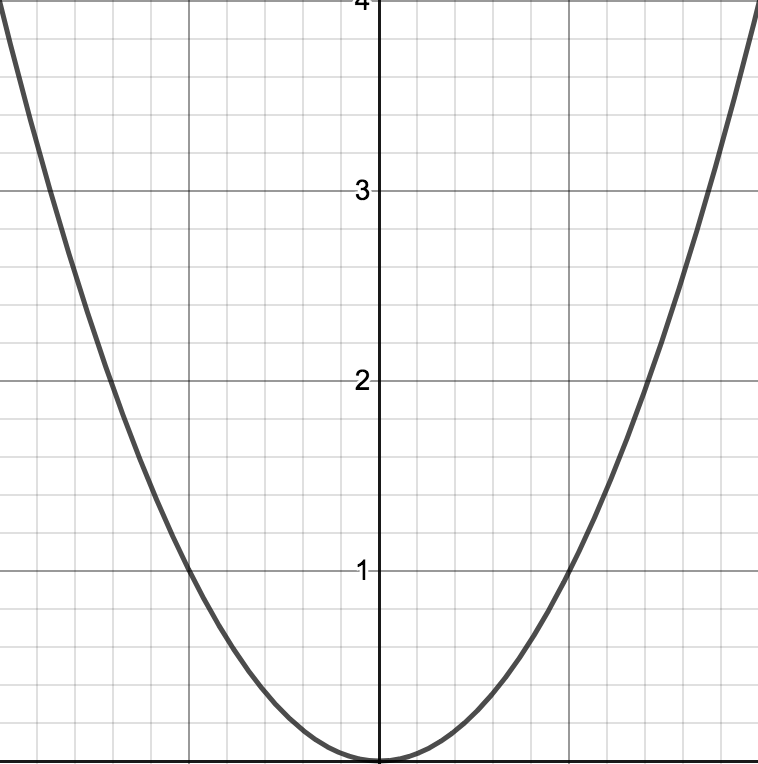
\includegraphics[width=0.5\textwidth]{36.png}
        \caption{Parabola: $ZY-X^2$.}
        \label{fig:subim1}
    \end{subfigure}
    \hfill
    \begin{subfigure}{0.5\textwidth}
        \centering
        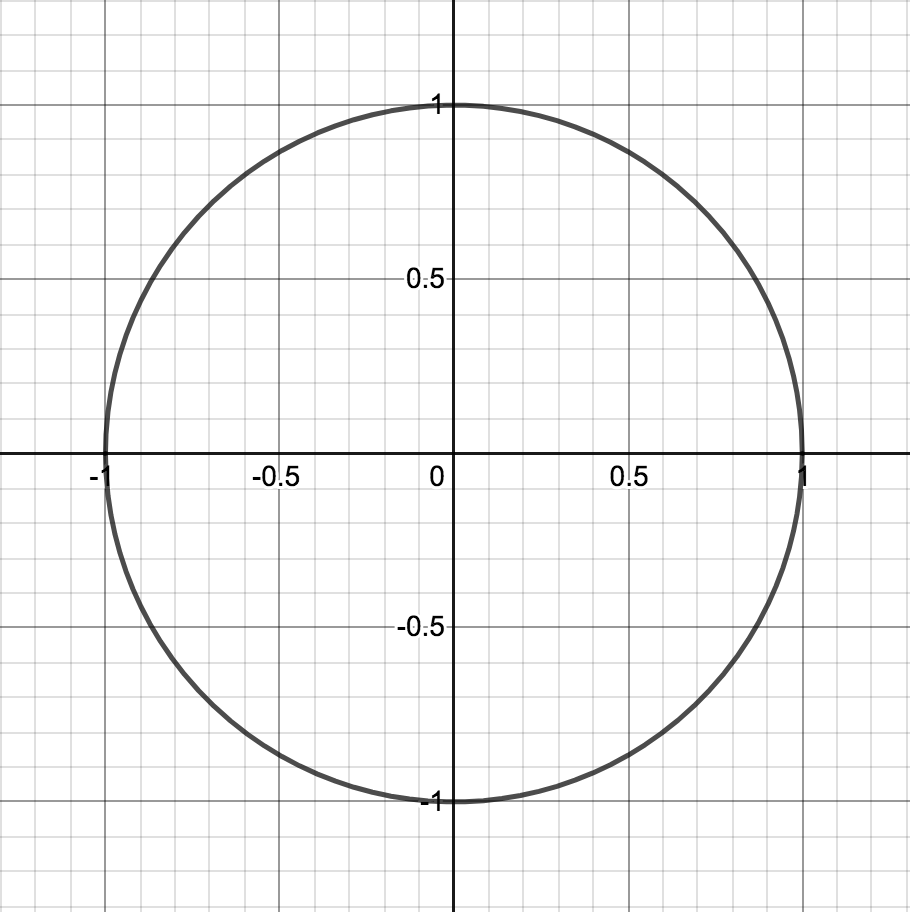
\includegraphics[width=0.5\textwidth]{37.png}
        \caption{Circle: $X^2+Y^2-Z^2$.}
        \label{fig:subim2}
    \end{subfigure}
    \vspace{1 cm}
    \begin{subfigure}{0.5\textwidth}
        \centering
        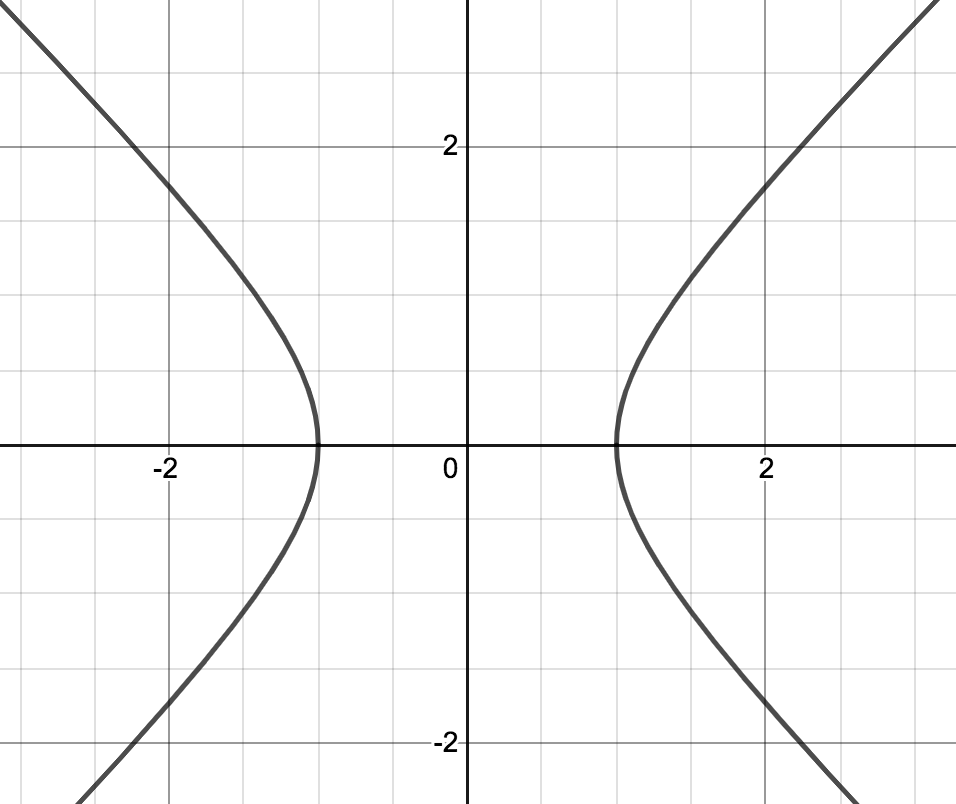
\includegraphics[width=0.5\textwidth]{38.png}
        \caption{Hyperbola: $X^2-Y^2-Z^2$.}
        \label{fig:subim2}
    \end{subfigure}
    \hfill
    \begin{subfigure}{0.5\textwidth}
        \centering
        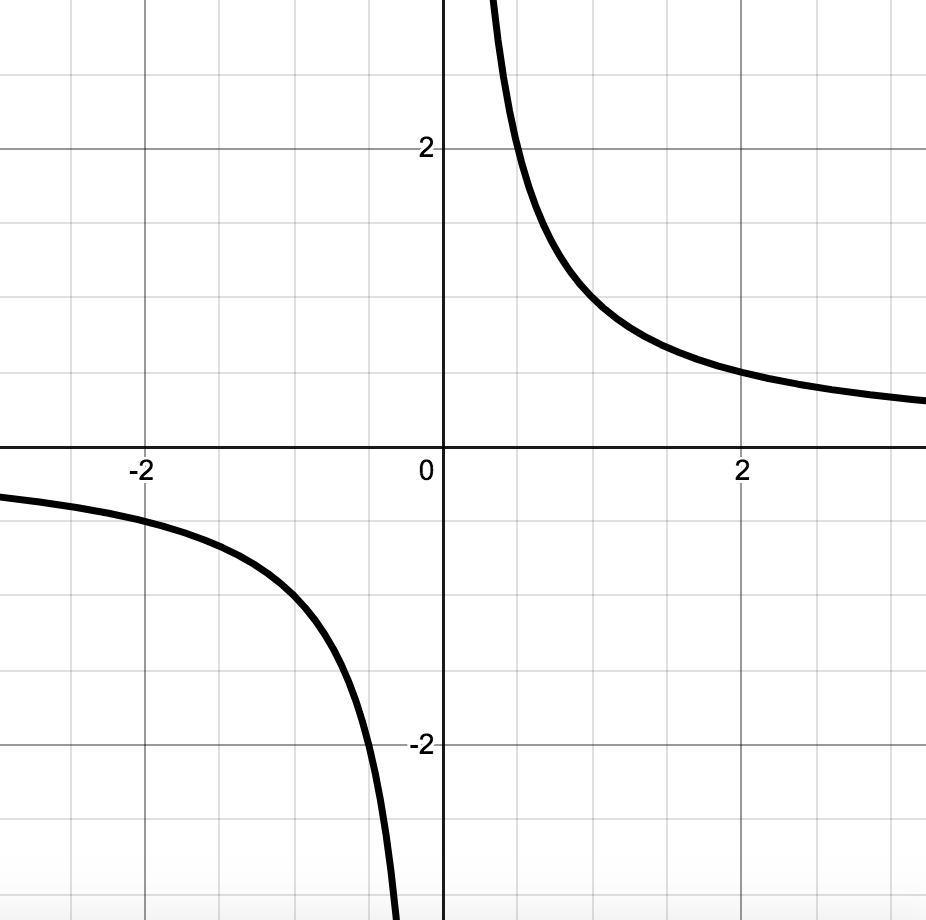
\includegraphics[width=0.5\textwidth]{39.png}
        \caption{$XY-Z^2$, which is just a rotated hyperbola.}
        \label{fig:subim2}
    \end{subfigure}

    \caption{Our favorite conics part 1. These are the \ita{irreducible} conics. Plotted in Desmos.}
\end{figure}
Note that in some of the graphs of the irreducible conics, there should also be infinite points included. 
\begin{enumerate}
    \item The parabola has infinite point $[0:1:0]$.
    \item The circle doesn't have any infinite points.
    \item The hyperbola has two: $[1:1:0]$ and $[1:-1:0]$.
    \item The rotated hyperbola also has two: $[0:1:0]$ and $[1:0:0]$.
\end{enumerate}
These infinite points ``close up'' the graph into a loop, and so there is really only one irreducible conic: $YZ-X^2$, which is also a closed loop!
\begin{figure}[H]
 
    \begin{subfigure}{0.5\textwidth}
        \centering
        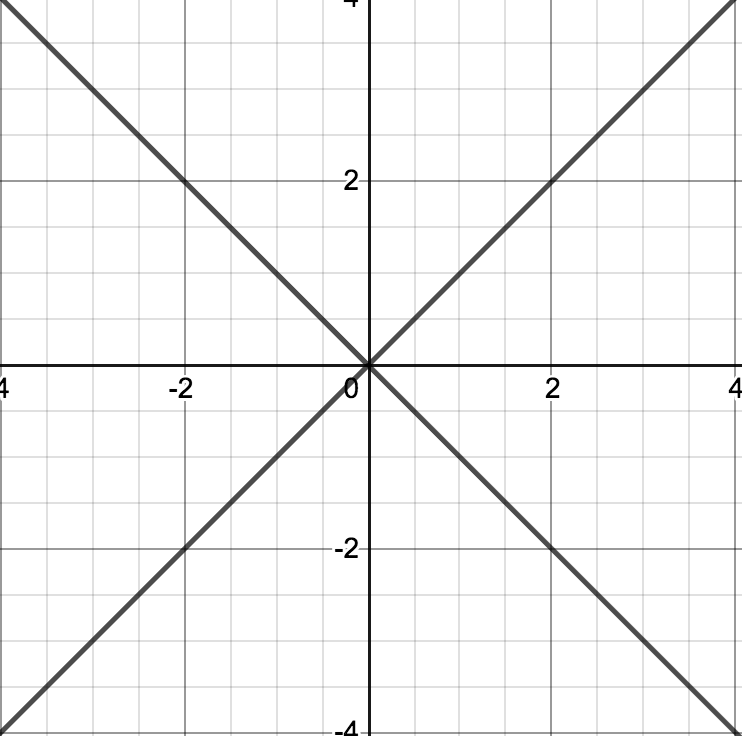
\includegraphics[width=0.5\textwidth]{40.png}
        \caption{Two lines: $Y^2-X^2=0$.}
        \label{fig:subim2}
    \end{subfigure}
    \hfill
    \begin{subfigure}{0.5\textwidth}
        \centering
        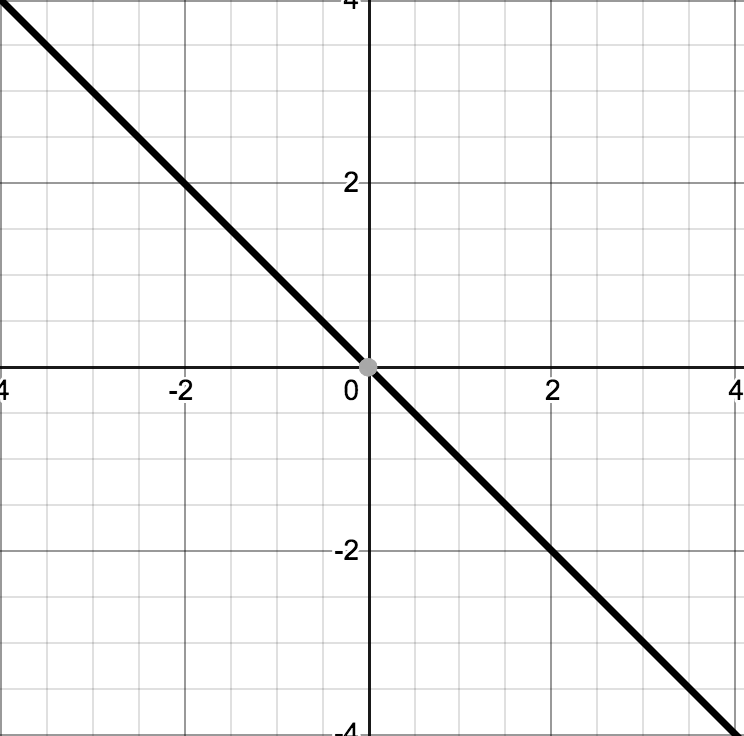
\includegraphics[width=0.5\textwidth]{41.png}
        \caption{Two lines again, though this time one of the lines is $L_{\infty}$: $(X+Y)Z=0$. }
        \label{fig:subim2}
    \end{subfigure}

    \caption{Our favorite conics part 2. These conics are not irreducible. Plotted in Desmos.}
    
\end{figure}
$Y^2-X^2$ also has tow infinite points: $[1:1:0]$ and $[1:-1:0]$. This one also closes up into a loop.

Next up, our favorite cubics:
\begin{enumerate}
    \item Elliptic curves: $F=ZY^2-X^3-bXZ^2-cZ^3$, for $a,b\in k$. 
    \item The Tschirnhausen cubic: $F=Y^2Z-X^3-X^2Z$.
    \item The cuspy boi: $F=Y^2Z-X^3$.
    \item Any product of three lines is a cubic.
    \item The product of a conic and a line is also a cubic.
\end{enumerate}
\begin{figure}[H]
 
    \begin{subfigure}{0.5\textwidth}
        \centering
        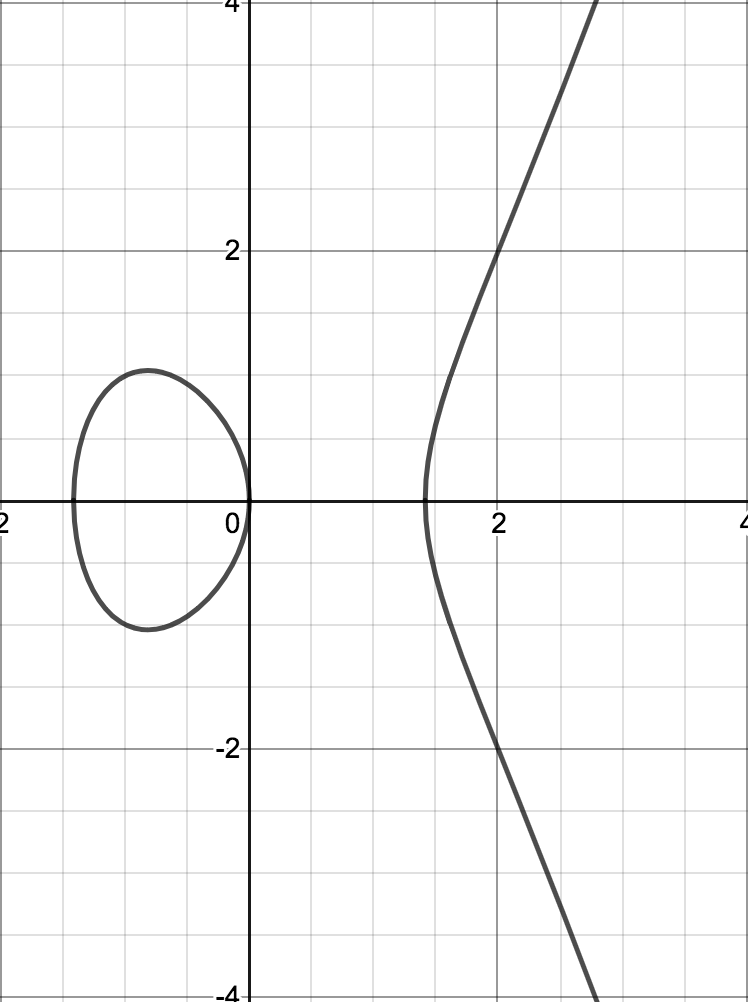
\includegraphics[width=0.5\textwidth]{42.png}
        \caption{Elliptic curve: $ZY^2-X^3+2XZ^2$.}
        \label{fig:subim1}
    \end{subfigure}
    \hfill
    \begin{subfigure}{0.5\textwidth}
        \centering
        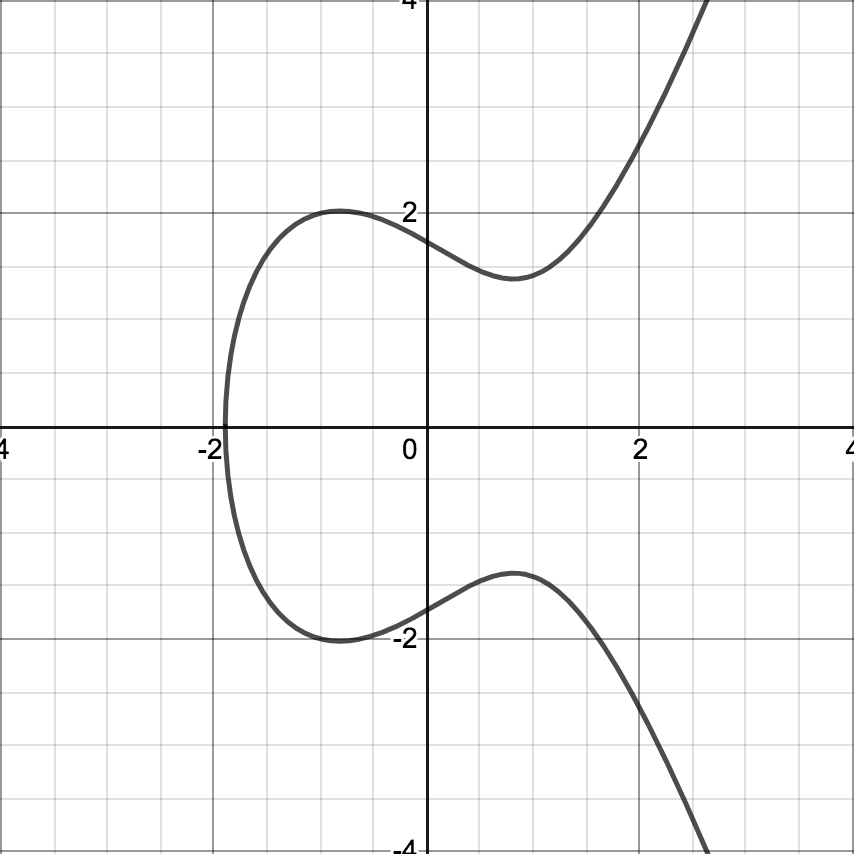
\includegraphics[width=0.5\textwidth]{47.png}
        \caption{Another elliptic curve: $ZY^2-X^3+2XZ^2+3Z^3$.}
        \label{fig:subim2}
    \end{subfigure}
    \vspace{1 cm}
    \begin{subfigure}{0.5\textwidth}
        \centering
        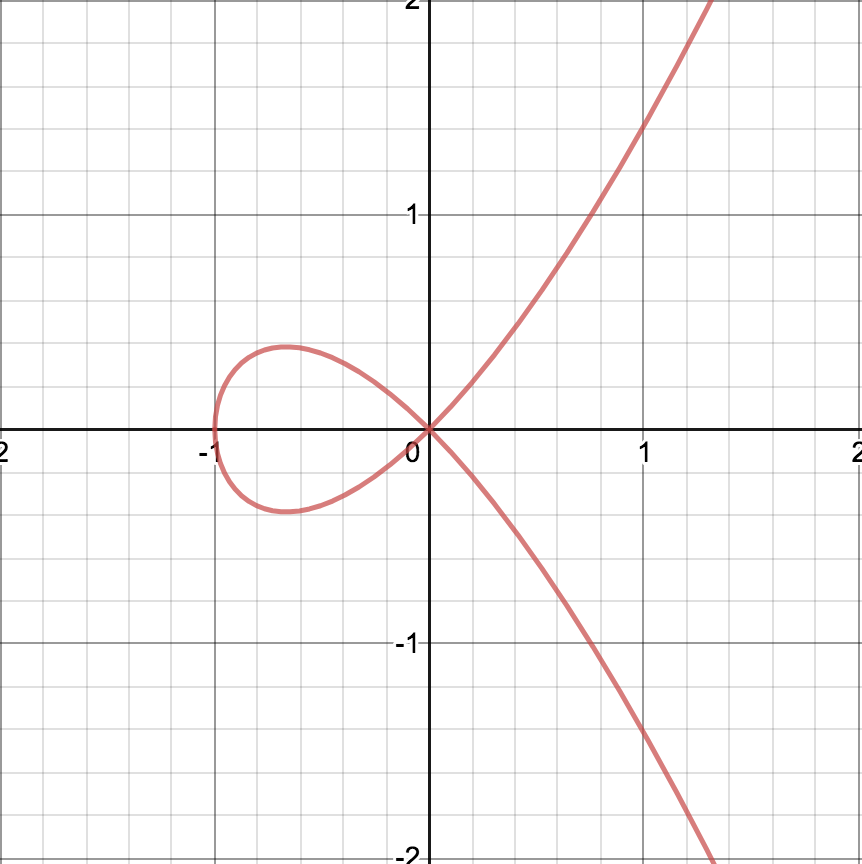
\includegraphics[width=0.5\textwidth]{43.png}
        \caption{Tschirnhausen cubic: $Y^2Z-X^3-X^2Z$.}
        \label{fig:subim2}
    \end{subfigure}
    \hfill
    \begin{subfigure}{0.5\textwidth}
        \centering
        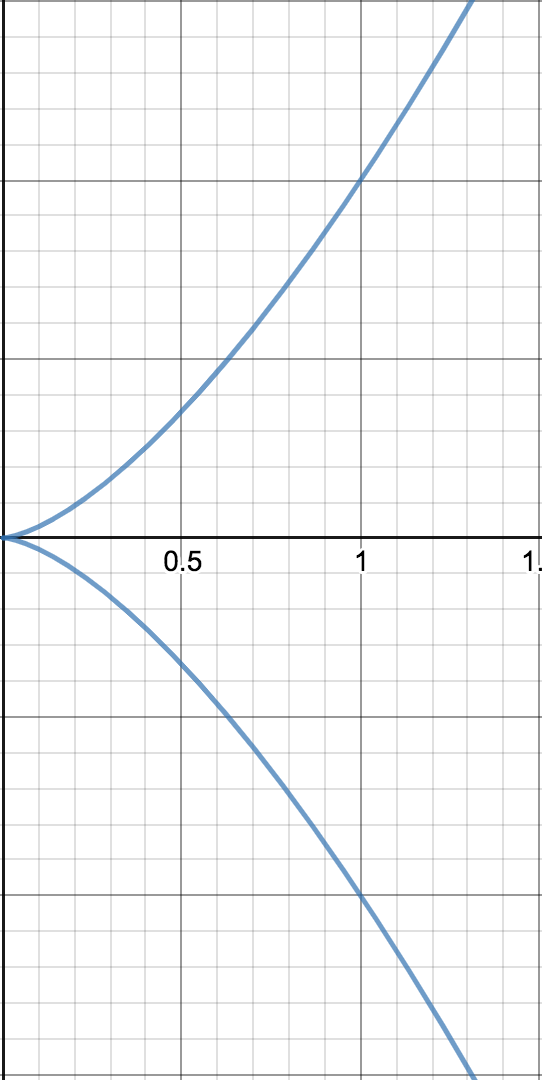
\includegraphics[width=0.5\textwidth]{46.png}
        \caption{The cuspy boi: $Y^2Z-X^3$.}
        \label{fig:subim2}
    \end{subfigure}
    \vspace{1 cm}
    \begin{subfigure}{0.5\textwidth}
        \centering
        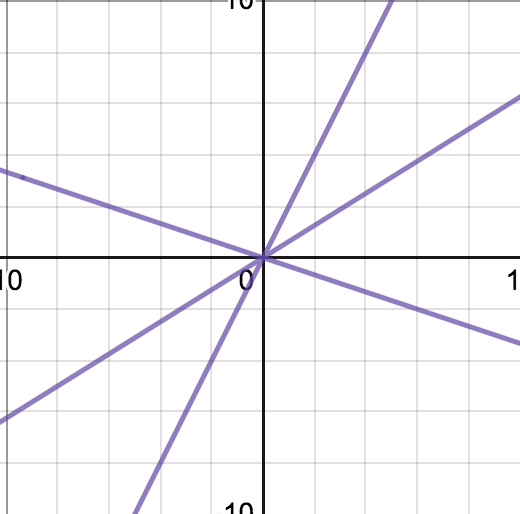
\includegraphics[width=0.5\textwidth]{44.png}
        \caption{Product of three lines.}
        \label{fig:subim2}
    \end{subfigure}
    \hfill
    \begin{subfigure}{0.5\textwidth}
        \centering
        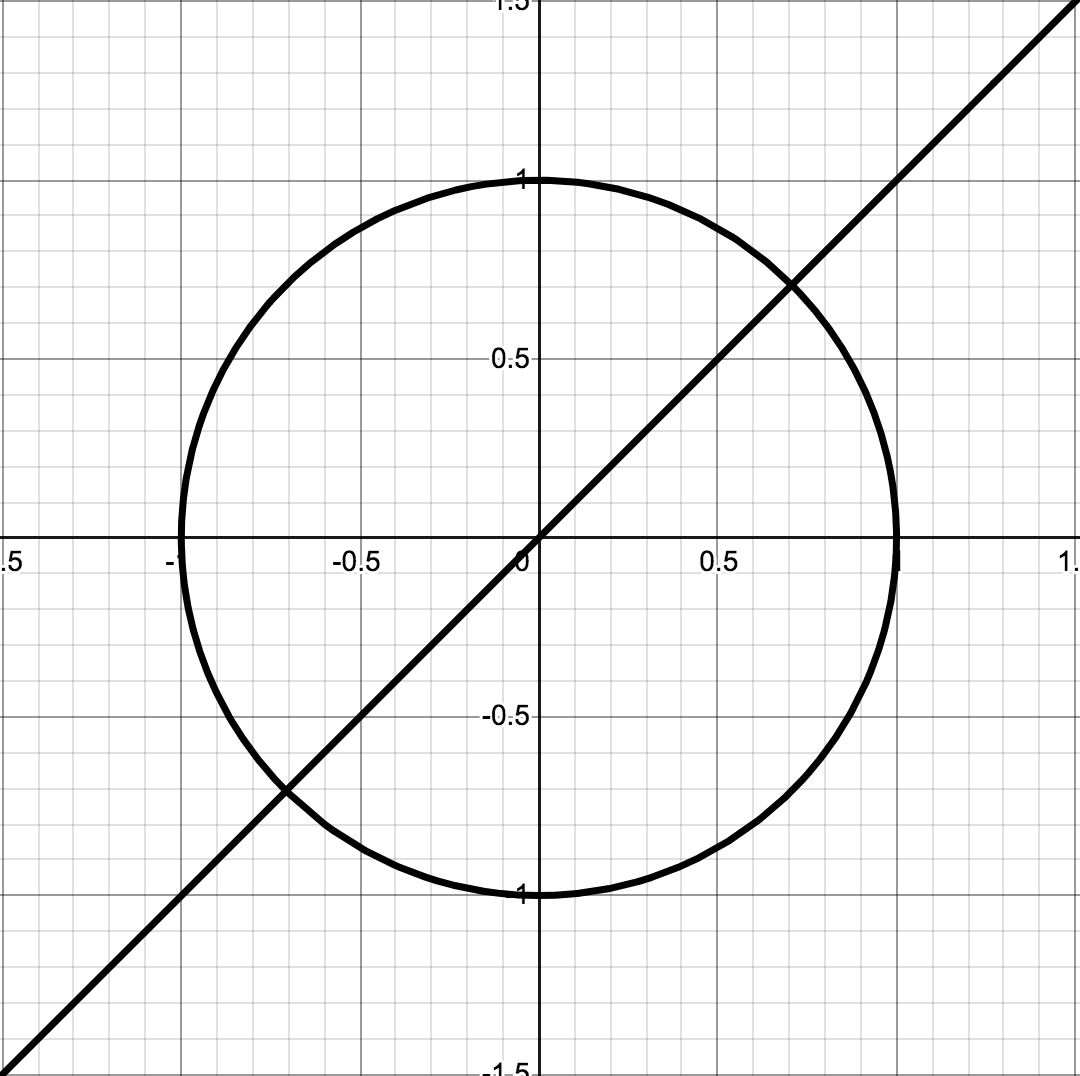
\includegraphics[width=0.5\textwidth]{45.png}
        \caption{Product of a circle and a line.}
        \label{fig:subim2}
    \end{subfigure}

    \caption{Our favorite cubics. Plotted in Desmos.}
\end{figure}
\begin{theorem}[Pascal's Theorem / Hexagrammum Mysticum]
    If a (not necessarily regular) hexagon is inscribed in an irreducible conic, then opposite sides meet in collinear points.
\end{theorem}
\begin{remark}
   ``Hexagon'' means any simple cyclic graph with six vertices, with overlapping edges!
\end{remark}
\section{01 May}
\subsection{Miniquiz}
Draw the hyperbola $XY=4$. Place the points
\begin{multicols}{3}
    \begin{itemize}
        \item $A:=(-4,-1)$
        \item $B:=(1,4)$
        \item $C:=(4,1)$
        \item $D:=(-1,-4)$
        \item $E:=(2,2)$
        \item $F:=(-2,-2)$
    \end{itemize}
\end{multicols}
in that order. Draw the Pascal Line. You should end up with something like the following:
\begin{figure}[H]
    \centering
    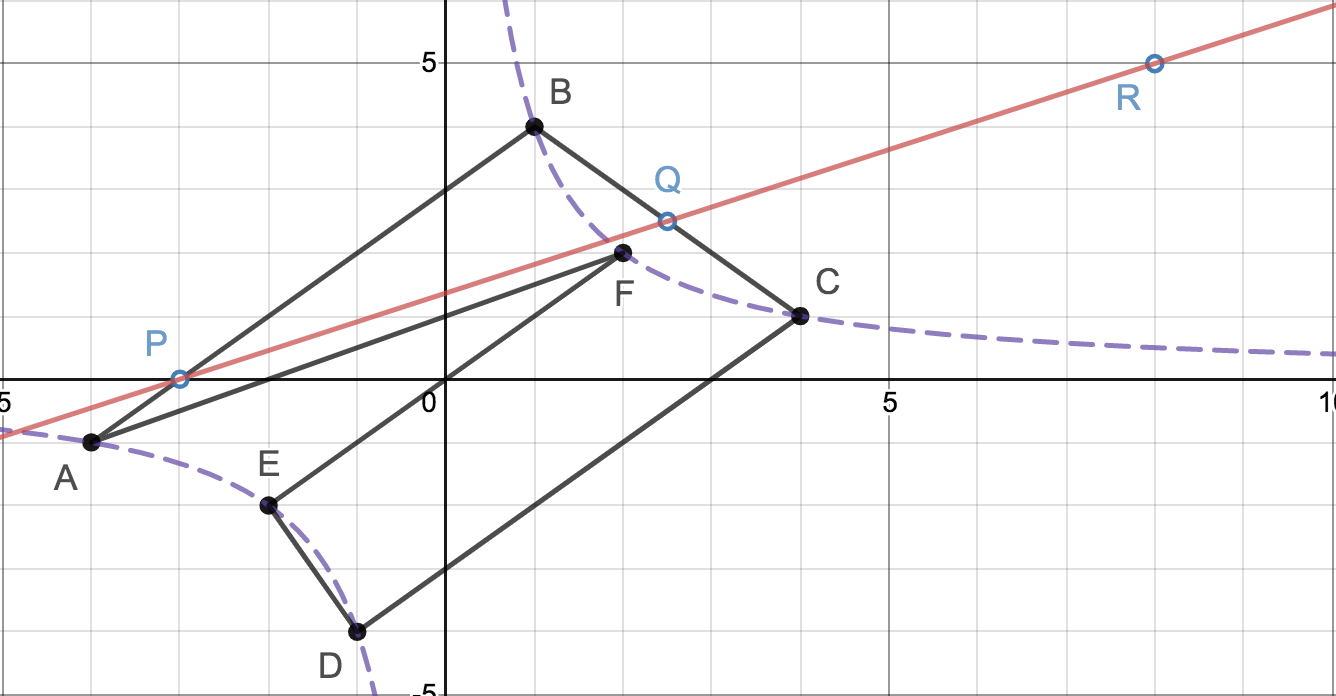
\includegraphics[width=0.5\textwidth]{48.png}
    \caption{Plotted in Desmos.}
\end{figure}
\subsection{From Last Time}
Recall the Slack Curve Theorem: Suppose that all points of $F\cap G$ are simple on $F$, and $H\cdot F\geq G\cdot F$. Then there is a curve $B$ such that $BG\cdot F=H\cdot F$. $B\cdot F$ takes up the slack intersections between $G\cdot F$ and $H\cdot F$.

Also recall Pascal's Theorem: If we inscribe a hexagon in an irreducible cubic, then opposite sides meet in collinear points. This theorem is circa 1639.

We are finally going to prove this with the tools built up from B\'ezout.
\begin{proof}
    Call your ``hexagon'' $abcdef$, inscribed on the conic $G$. Pascal looks at the points
    \[P:=L_{ab}\cap L_{ed},\quad Q:=L_{ef}\cap L_{bc},\quad R:=L_{cd}\cap L_{fa}.\]
    Define 
    \[F:=(L_{ab})(L_{ef})(L_{cd}),\qquad H:=(L_{ed})(L_{bc})(L_{fa}).\]
    To find intersections, intersect each line with each line. Then
    \begin{align*}
        H\cdot F&=(P+b+a)+(e+Q+f)+(d+c+R)\\
        G\cdot F&=a+b+c+d+e+f.
    \end{align*}
    Then $H\cdot F\geq G\cdot F$. By Slack Curve Theorem, there is a curve $B$ such that $BG\cdot F=H\cdot F$. Then $B\cdot F+G\cdot F=H\cdot F$, and so $B\cdot F=P+Q+R$. By B\'ezout's Theorem, $B$ must be a line. So $P$, $Q$, and $R$ are collinear.
\end{proof}
\subsection{More Old Theorems}
\begin{theorem}[Pappus' Theorem, c. 290 AD]
    Let $L_1$ and $L_2$ be two distinct lines, $P_1$, $P_2$, $P_3$ be three distinct points on $L_1$, and $Q_1$, $Q_2$, $Q_3$ be three distinct points on $L_2$. Let
    \[R_1:=P_2Q_3\cap Q_2P_3,\quad R_2:=P_1Q_3\cap Q_1P_3,\quad R_3:=P_1Q_2\cap Q_1P_2.\]
    Then $R_1$, $R_2$, and $R_3$ are collinear.
\end{theorem}
For example, let $L_1=3X-4Y$, $L_2=X+2Y$. and choose
\begin{multicols}{2}
    \begin{itemize}
        \item $P_1:=\left(-2,-\frac{3}{2}\right)$
        \item $P_2:=\left(-1,-\frac{3}{4}\right)$
        \item $P_3:=\left(-\frac{12}{25},-\frac{9}{25}\right)$
        \item $Q_1:=(-2,1)$
        \item $Q_2:=\left(-1,\frac{1}{2}\right)$
        \item $Q_3:=\left(-\frac{1}{2},\frac{1}{4}\right)$
    \end{itemize}
\end{multicols}
Then the points
\[R_1=\left(-\frac{25}{38},-\frac{5}{76}\right),\quad R_2=\left(-\frac{37}{47},-\frac{4}{47}\right),\quad R_3=\left(-\frac{4}{3},-\frac{1}{6}\right)\]
formed from above all lie on the line $23X-154Y+5Z$.
\begin{figure}[H]
    \centering
    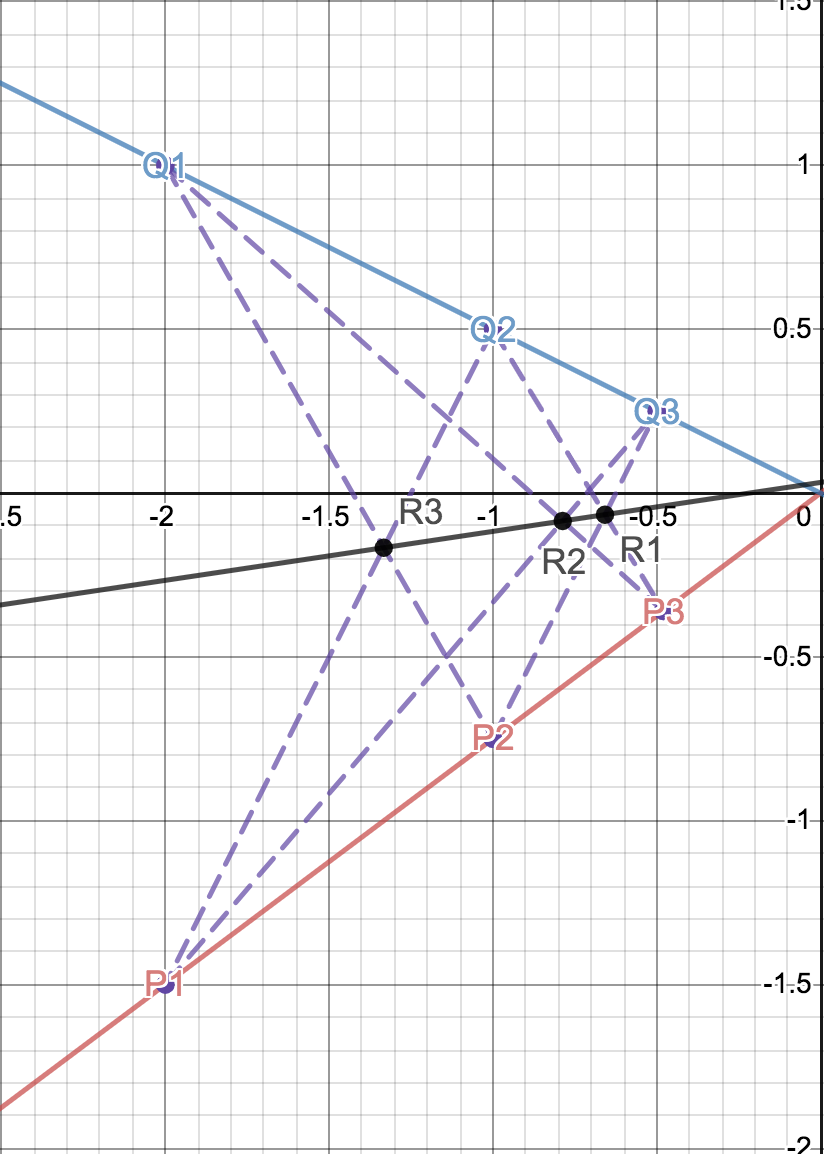
\includegraphics[height = 8 cm]{49.png}
    \caption{Example of Pappus' Theorem. Plotted in Desmos.}
\end{figure}
\begin{proof}
    This is actually the non-irreducible case of Pascal, where the hexagon is $P_1Q_2P_3Q_1P_2Q_3$. Then the opposite intersections are $R_1$, $R_2$, and $R_3$.
\end{proof}
\begin{theorem}[Cayley-Bacharach Theorem / Nine-Point Theorem, 1886]
    Let $F$, $G$, and $C$ be cubics with no common components. Suppose $G\cdot F=\sum\limits_{i=1}^nP_i$, where $P_i$ are simple on $F$. Suppose $C\cdot F=Q+\sum\limits_{i=1}^8P_i$. Then $Q=P_9$, \ita{i.e.}, if $C\cdot F$ contains eight of the nine intersections of $F$ and $G$, then $C$ contains the ninth one also.
\end{theorem}
\begin{proof}
    Suppose, to form a contradiction, that $Q\neq P_9$. Find any line containing $L$ but not $Q$. Then $L\cdot F=P_9+R+S$ for some $R,S\in\mathbb{P}^2$. Then
    \begin{align*}
        LC\cdot F&=L\cdot F+L\cdot C\\
        &=P_9+R+S+Q+\sum\limits_{i=1}^8P_i\\
        &=R+S+Q+\sum\limits_{i=1}^9P_i\\
        &=R+S+Q+G\cdot F.
    \end{align*}
    Then $LC\cdot F\geq G\cdot F$. By Slack Curve (letting $H=LC$), there exists a $B$ such that $BG\cdot F=LC\cdot F\Rightarrow B$ is a line. So $B\cdot F=R+S+Q$. So $R$, $S$, and $Q$ are collinear. But the line through $R$ and $S$ is $L$, contradicting the construction of $L$. So $Q=P_9$.
\end{proof}
\section{06 May}
\subsection{Miniquiz}
Draw the parabola $Y=X^2$. \underline{In order}, place the points:
\begin{multicols}{2}
    \begin{itemize}
        \item $A:=(0,0)$
        \item $B:=(0,0)$
        \item $C:=(2,4)$
        \item $D:=(-2,4)$
        \item $E:=(1,1)$
        \item $F:=(-3,9)$
    \end{itemize}
\end{multicols}
Draw the Pascal line.
\subsection{Elliptic Curves}
Recall Cayley-Bacharach: Let $F$, $G$, $E$ (today $C$ became $E$) be cubics. If $E$ contains 8 of the 9 intersections of $F$ and $G$, then it contains the ninth one.
\begin{definition}
    An \ita{elliptic curve} is of the form $E:=Y^2-\text{cubic in }X$. If $k$ is algebraically closed, then we can write $E=Y^2-(X-a)(X-b)(X-c)$.
\end{definition}
How do we sketch the graph of such a cubic? First, start off with a sketch of $Y=(X-a)(X-b)(X-c)$.
\begin{figure}[H]
    \centering
    \includegraphics[width=0.5\textwidth]{50.png}
    \caption{$Y=(X-1)(X-2)(X-3)$. Plotted in Desmos.}
\end{figure}
To sketch $Y^2=(X-a)(X-b)(X-c)$, sketch both roots of $(X-a)(X-b)(X-c)$, and leave out the portions where the graph dips below the $X$-axis.
\begin{figure}[H]
    \centering
    \includegraphics[width=0.5\textwidth]{51.png}
    \caption{$Y^2=(X-1)(X-2)(X-3)$. Plotted in Desmos.}
\end{figure}
Let $P,Q\in V(E)\subset\mathbb{P}^2$. Then the line $PQ$ must intersect the curve again (thanks B\'ezout!) Call that point $P*Q$. We reflect $P*Q$ across the $X$-axis (change $Y$ to $-Y$). Call that new point ``$P+Q$.''
\begin{figure}[H]
    \centering
    \includegraphics[width=0.5\textwidth]{52.png}
    \caption{``$P+Q$.'' Plotted in Desmos. Note that the scale of the axes has been skewed to better accommodate the figure.}
\end{figure}
\underline{Astonishing Fact}: Let $k$ be any field (not even algebraically closed). Favorite examples include $\q$, $\real$, $\cx$, finite fields. Then under this ``addition,'' $V(E)$ is an abelian group!

Hold on, it this even well-defined? Yes, and the justification is due to B\'ezout, more or less.
\begin{enumerate}
    \item \underline{closure}: If $P,Q\in V(E)$, then $P+Q\in V(E)$. \checkmark
    \item \underline{associativity}: Highly dubious!
    \item \underline{identity}: The infinite point $\infty:=[0:1:0]$ is the identity element. \checkmark
    \item \underline{inverses}: Let $P:=(X,Y)$. Then $(X,-Y)\in V(E)$ and $(X,-Y)+P=\infty$. \checkmark
    \item \underline{abelianity}: $PQ$ and $QP$ define the same line. \checkmark
\end{enumerate}
\begin{claim}
    Associativity holds.
\end{claim}
\begin{proof}
    Construct three cubics:
    \begin{itemize}
        \item $F:=(PQ)[(Q+R)\infty][(P+Q)R]$
        \item $G:=(QR)[(P+Q)\infty][(Q+R)P]$
        \item $E:=$ elliptic curve
    \end{itemize}
    $F$ and $G$ have 9 intersections by B\'ezout, which we can list by intersecting each pair of lines:
    \[
        \begin{tabular}{|| c | c | c ||}
        \hline
        $PQ$ & $(Q+R)\infty$ & $(P+Q)R$ \\
        \hline
        $QR$ & $R*Q$ & $R$ \\
        $(P+Q)\infty$ & $\infty$ & $P+Q$ \\
        $(Q+R)P$ & $Q+R$ & mystery point? \\
        \hline
        \end{tabular}
    \]
    By Cayley-Bacharach, $E$ passes through the mystery point, which is
    \begin{align*}
        (P+Q)*R&=(Q+R)*P\\
        \Rightarrow(P+Q)+R&=(Q+R)+P\\
        &=P+(Q+R).
    \end{align*}
\end{proof}
Now we spend all of MATH 541 exploring that group $V(E)$.

Some sample theorems:
\begin{enumerate}
    \item If $k=\cx$, then $V(E)$ is a torus.
    \item If $k=\q$, then $V(E)$ is a \ita{finitely generated / finitely presented abelian group.} So
    \begin{equation}
        V(E)\cong\underbrace{\z^r}_{\text{free part}}\oplus\underbrace{T}_{\text{torsion part}}.
    \end{equation}
    By the structure theorem of abelian groups, 
    \begin{equation}
        T\cong\bigoplus\limits_{i=1}^m\z_{p_i^{t_i}}.
    \end{equation}
    $T$ is well understood in MATH 541. But there are still several open questions about the rank $r$, and is the subject of current research.
    \item If $k$ is finite, then $V(E)$ will also be finite and useful for cryptography (both encryption and decryption), the Millenium Problems, Andrew Wiles' proof of Fermat's Last Theorem, \ita{etc}.
\end{enumerate}
\end{document}